\documentclass[12pt,a4paper]{book}
%宏包
\usepackage{amsmath}%数学符号
\usepackage{amssymb}%数学符号
\usepackage{amsthm}%数学符号
\usepackage{geometry}%界面布局
\usepackage{natbib}%bibtex
\usepackage{tikz}%交换图
\usepackage{tikz-cd}%交换图
\usepackage{quiver}%交换图
\usepackage{float}%浮动体固定
\usepackage{caption}%图片标题
\usepackage[colorlinks,linkcolor=blue]{hyperref}%超链接
\usepackage{enumerate}%计数列表
\usepackage{tabularx}%控制列宽
\usepackage{xr}%跨文件引用
\externaldocument{D:/latex/book/algebra/algebra}
\externaldocument{D:/latex/book/analysis/analysis}
\usepackage{CTEX}
\ctexset{today=old,contentsname=Contents}
   
%页面设置
\linespread{1.2}
\geometry{a4paper,left=2cm,right=2cm,top=2.5cm,bottom=2cm}
%\geometry{a4paper,left=2cm,right=2cm,top=2.5cm,bottom=2cm}

%环境和宏指令
\newenvironment{prooff}{{\noindent\it\textcolor{cyan!40!black}{Proof}:}\,}{\par \vskip 1cm}
\newenvironment{proofff}{{\noindent\it\textcolor{cyan!40!black}{Proof of the lemma}:}\,}{\qed \par}
\newcommand{\bbrace}[1]{\left\{ #1 \right\} }
\newcommand{\bb}[1]{\mathbb{#1}}
\newcommand{\p}{^{\prime}}
\renewcommand{\mod}[1]{(\text{mod}\,#1)}
\newcommand{\blue}[1]{\textcolor{blue}{#1}}
\newcommand{\spec}[1]{\text{Spec}({#1})}
\newcommand{\rarr}[1]{\xrightarrow{#1}}
\newcommand{\larr}[1]{\xleftarrow{#1}}
\newcommand{\emptyy}{\underline{\quad}}
\newenvironment{enu}{\begin{enumerate}[(1)]}{\end{enumerate}}
%ctrl+点击文本返回代码  选中代码 ctrl+alt+j 为代码查找文本

%定理环境
\theoremstyle{definition}
\newtheorem{defn}{Definition}[section]
\newtheorem{coro}[defn]{Corollary}
\newtheorem{theo}[defn]{Theorem}
\newtheorem{exer}[defn]{Exercise}
\newtheorem{rema}[defn]{Remark}
\newtheorem{lem}[defn]{Lemma}
\newtheorem{prop}[defn]{Proposition}
\newtheorem{nota}[defn]{Notation}
\newtheorem{exam}[defn]{Example}


\begin{document}
\title{Number Theory}
\author{Erzhuo Wang}
\date{\today}
% \thispagestyle{empty}
% \begin{figure}
%     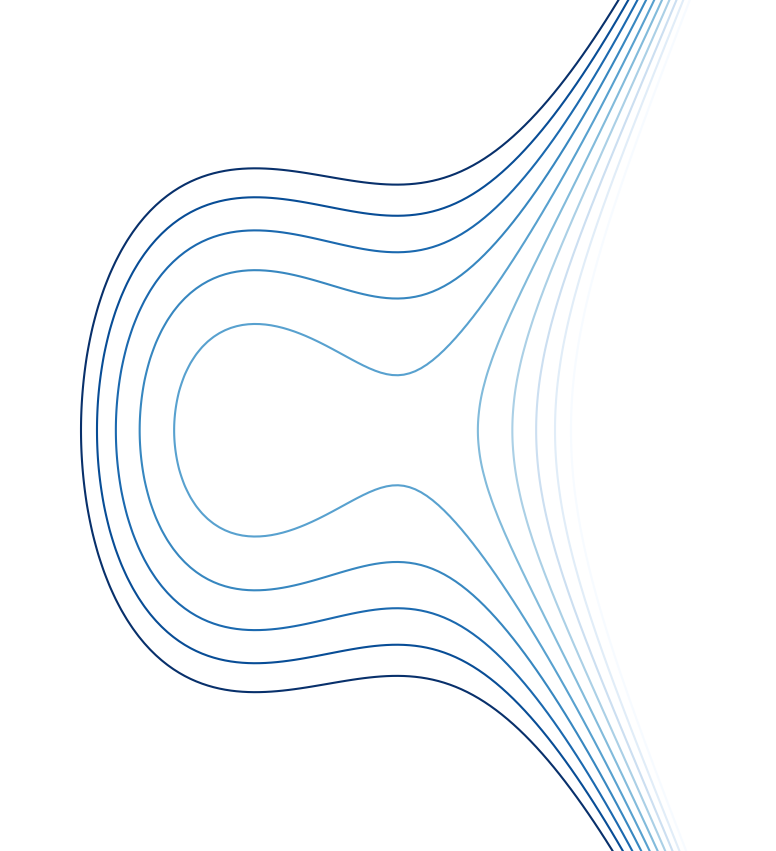
\includegraphics{cover.png}
%     \centering
% \end{figure}
\maketitle
\tableofcontents
\chapter{Global Field}
% \begin{equation*}
%     \lim_{s \rightarrow 1}(s-1) \zeta_K(s)=\frac{2^{r_1} \cdot(2 \pi)^{r_2} \cdot R_K \cdot h_K}{w_K \cdot \sqrt{\left|d_K\right|}}
% \end{equation*}
% \begin{equation*}
%     \sum_{n=-\infty}^{\infty} f(x+n)=\sum_{n=-\infty}^{\infty} \widehat{f}(n) e^{2\pi i n x}
% \end{equation*}
\section{Trace and Norm}
\begin{defn}[Trace and Norm]
    $L/K$ finite fields extension. The trace and norm of an element $x \in L$ are defined to be the trace and determinant, respectively, of the endomorphism
    $$
        T_x: L \rightarrow L, \quad T_x(\alpha)=x \alpha,
    $$
    of the $K$-vector space $L$ :
    $$
        \operatorname{Tr}_{L \mid K}(x)=\operatorname{Tr}\left(T_x\right), \quad N_{L \mid K}(x)=\operatorname{det}\left(T_x\right) .
    $$
\end{defn}
\begin{prop}
    In the characteristic polynomial
    $$
        f_x(t)=t^n+a_{n-1}t^{n-1}+\dots+ a_0 \in K[t]
    $$
    of $T_x, n=[L: K]$, we recognize the trace and the norm as
    $$
        -a_{n-1}=\operatorname{Tr}_{L \mid K}(x) \text { and } (-1)^na_0=N_{L \mid K}(x) .
    $$

    Since $T_{x+y}=T_x+T_y$ and $T_{x y}=T_x \circ T_y$, we obtain homomorphisms
    $$
        \operatorname{Tr}_{L \mid K}: L \longrightarrow K \quad \text { and } \quad N_{L \mid K}: L^* \longrightarrow K^* \text {. }
    $$
\end{prop}
\begin{prop}
    If $L/K$ is a finite separable extension, 
    the characteristic polynomial $f_x(t)$ is a power
    $$
    f_x(t)=p_x(t)^d, \quad d=[L: K(x)]
    $$
    of the minimal polynomial
    $$
    p_x(t)=t^m+c_1 t^{m-1}+\cdots+c_m, \quad m=[K(x): K]
    $$
    of $x$.
    \label{proposition:power of minimal poly} 
\end{prop}
\begin{prooff}
    In fact, $1, x, \ldots, x^{m-1}$ is a basis of $K(x)/K$, and 
    if $\alpha_1, \ldots, \alpha_d$ is a basis of $L/K(x)$, then
$$
\alpha_1, \alpha_1 x, \ldots, \alpha_1 x^{m-1} ; \ldots ; \alpha_d, \alpha_d x, \ldots, \alpha_d x^{m-1}
$$
is a basis of $L/K$.
\end{prooff}
\begin{prop}
    If $L/K$ is a finite separable extension and $\sigma: L \rightarrow \bar{K}$ varies over the different $K$-embeddings of $L$ into an algebraic closure $\bar{K}$ of $K$, then we have
    \begin{enu}
        \item $f_x(t)=\prod_\sigma(t-\sigma x)$,
        \item $\operatorname{Tr}_{L \mid K}(x)=\sum_\sigma \sigma x$,
        \item $N_{L \mid K}(x)=\prod_\sigma \sigma x$.
    \end{enu}
\end{prop}
\begin{prop}
    The discriminant of a basis $\alpha_1, \ldots, \alpha_n$ of a separable extension $L \mid K$ is defined by
    $$
        d\left(\alpha_1, \ldots, \alpha_n\right)=\operatorname{det}\left(\left(\sigma_i \alpha_j\right)\right)^2
    $$
    where $\sigma_i, i=1, \ldots, n$, varies over the $K$-embeddings $L \rightarrow \bar{K}$. Because of the relation
    $$
        \operatorname{Tr}_{L \mid K}\left(\alpha_i \alpha_j\right)=\sum_k\left(\sigma_k \alpha_i\right)\left(\sigma_k \alpha_j\right),
    $$
    the matrix $\left(\operatorname{Tr}_{L \mid K}\left(\alpha_i \alpha_j\right)\right)$ is the product of the matrices $\left(\sigma_k \alpha_i\right)^t$ and $\left(\sigma_k \alpha_j\right)$. Thus one may also write
    $$
        d\left(\alpha_1, \ldots, \alpha_n\right)=\operatorname{det}\left(\operatorname{Tr}_{L \mid K}\left(\alpha_i \alpha_j\right)\right) .
    $$

    In the special case of a basis of type $1, \theta, \ldots, \theta^{n-1}$ one gets
    $$
        d\left(1, \theta, \ldots, \theta^{n-1}\right)=\prod_{i<j}\left(\theta_i-\theta_j\right)^2,
    $$
    where $\theta_i=\sigma_i \theta$.
\end{prop}
\begin{rema}
    Consider a finite separable extenison $L/K$, $(x,y)=\text{Tr}_{L/K}(xy)$ is a bi-linear function from $L\times L$ to $K$.
    Above Proposition tells us this bi-linear function is non-degenerated. Hence for any basis $\bbrace{\alpha_1,\dots,\alpha_n}$,
    $$
        d\left(\alpha_1, \ldots, \alpha_n\right)\neq 0
    $$
\end{rema}
\begin{prop}
    Integrally closed integral domain $A$ with field of fractions $K$, and to its integral closure $B$ in the finite separable extension $L \mid K$. If $x \in B$ is an integral element of $L$, then all of its conjugates $\sigma x$ are also integral. Taking into account that $A$ is integrally closed, i.e., $A=B \cap K$ implies that
    $$
        \operatorname{Tr}_{L/K}(x), \quad N_{L/K}(x) \in A
    $$

    Furthermore, for the group of units of $B$ over $A$, we obtain the relation
    $$
        x \in B^* \Longleftrightarrow N_{L/K}(x) \in A^* .
    $$
\end{prop}
\begin{lem}
    Let $\alpha_1, \ldots, \alpha_n$ be a basis of $L/K$ which is contained in $\mathcal{O}_L$, of discriminant $d=d\left(\alpha_1, \ldots, \alpha_n\right)$. Then one has
    $$
        d\mathcal{O}_L\subseteq\mathcal{O}_K \alpha_1+\cdots+\mathcal{O}_K  \alpha_n
    $$
    More generally, if $O_K$ be an integral domain, 
    $K$ be its fraction field,$L/K$ be a separable extension  
    and $O_L$ be its integral closure, this Lemma also holds.
    \label{lemma: discriminant and OL,OK}
\end{lem}
\begin{prooff}
    If $\alpha=a_1 \alpha_1+\cdots+a_n \alpha_n \in \mathcal{O}_L, a_j \in K$, then the $a_j$ are a solution of the system of linear equations
    $$
        \operatorname{Tr}_{L \mid K}\left(\alpha_i \alpha\right)=\sum_j \operatorname{Tr}_{L \mid K}\left(\alpha_i \alpha_j\right) a_j,
    $$
\end{prooff}
\begin{defn}[integral basis]
    $K$ is an algebraic number field with degree $n$ and all the algebraic integer in $K$ form a subring of $K$, denoted it by $\mathcal{O}_K$.
    For any ideal $I$ of $\mathcal{O}_K$, there's a basis $\omega_1,\omega_2,\dots,\omega_n$ for $K/\bb{Q}$
    such that $w_i,i=1,\dots,n\in  \mathcal{O}_K$ and $I=\bb{Z}\omega_1\oplus \dots \oplus \bb{Z}\omega_n$. In particular, every
    ideal of $O_K$ is a free $\bb{Z}$-module of rank $n$. We call basis of $O_K$ as free abelian group integral basis of $\mathcal{O}_K$
\end{defn}
\begin{defn}[discriminant of number field]
    Define $d_K=d(\omega_1,\omega_2,\dots,\omega_n)$, where $\omega_1,\omega_2,\dots,\omega_n$ is an integral basis of $\mathcal{O}_K$.
\end{defn}
\begin{prop}
    Let $L/ \bb{Q}$ and $L^{\prime}/\bb{Q}$ be two Galois extensions of degree $n$, resp. $n^{\prime}$, such that $L \cap L^{\prime}=K$. Let $\omega_1, \ldots, \omega_n$,
    resp. $\omega_1^{\prime}, \ldots, \omega_{n^{\prime}}^{\prime}$,
    be an integral basis of $L \mid \bb{Q}$, resp. $L^{\prime} \mid \bb{Q}$, with discriminant $d$, resp. $d^{\prime}$.
    Suppose that $d$ and $d^{\prime}$ are relatively prime. Then $\omega_i \omega_j^{\prime}$ is an integral basis of $L L^{\prime}$, of discriminant $d^{n^{\prime}} d^{\prime n}$.
\end{prop}
\begin{exam}{integral basis of quadratic number field}
    Let $D$ be a squarefree rational integer $\neq 0,1$ and $d$ the discriminant of the quadratic number field $K=\mathbb{Q}(\sqrt{D})$. Show that
    $$
        \begin{array}{ll}
            d=D,   & \text { if } D \equiv 1 \bmod 4,                \\
            d=4 D, & \text { if } D \equiv 2 \text { or } 3 \bmod 4,
        \end{array}
    $$
    and that an integral basis of $K$ is given by $\{1, \sqrt{D}\}$ in the second case, by $\left\{1, \frac{1}{2}(1+\sqrt{D})\right\}$ in the first case, and by $\left\{1, \frac{1}{2}(d+\sqrt{d})\right\}$ in both cases.
\end{exam}
\begin{theo}
    Assume $f(x)=x^n+\alpha x+b \in \mathbb{Q}[x]$ is a irreducible polynomial, $\theta$ is a root of $f(x)$. Then $\mathbb{Q}(\theta)$ is an algebraic number field. In the extension $\mathbb{Q}(\theta)/\mathbb{Q}$,
    \begin{equation*}
        d(1,\theta,\dots,\theta^{n-1})=
        d(f)=(-1)^{n(n-1)/2}\left[(-1)^{n-1}(n-1)^{n-1} a^n+n^n b^{n-1}\right]
    \end{equation*}
    In particular, when $n=3$, $d(1,\theta,\theta^2)=-\left(4 a^3+27 b^2\right)$.
\end{theo}
\begin{prop}
    The ring $\mathcal{O}_K$ is noetherian, integrally closed, and $\dim \mathcal{O}_K=1$.
\end{prop}
\begin{prooff}
    Noetherian:since every ideal is a free $\bb{Z}$-module of rank $[K:\bb{Q}]$.

    integrally closed: $\alpha\in K$ integral over $\mathcal{O}_K$, then $\mathcal{O}_K[\alpha]$ is integral over $\mathcal{O}_K$, hence over $\bb{Z}$.

    $\dim =1$: It thus remains to show that each prime ideal $p \neq 0$ is maximal. Now, $p \cap \mathbb{Z}$ is a nonzero prime ideal $(p)$ in $\mathbb{Z}$ : the primality is clear, and if $y \in \mathfrak{p}, y \neq 0$, and
    $$
        y^n+a_1 y^{n-1}+\cdots+a_n=0
    $$
    is an equation for $y$ with $a_i \in \mathbb{Z}, a_n \neq 0$, then $a_n \in \mathfrak{p} \cap \mathbb{Z}$. The integral domain $\overline{\mathcal{O}}=\mathcal{O}_K / \mathfrak{p}$ is a field also follows from above equation.
\end{prooff}
\begin{prop}
    \begin{enu}
        \item
        $$
            \mathfrak{N}((\alpha))=\left|N_{K \mid \mathbb{Q}}(\alpha)\right|
        $$
        \item
        If $\mathfrak{a}=\mathfrak{p}_1^{\nu_1} \cdots \mathfrak{p}_r^{\nu_r}$ is the prime factorization of an ideal $a \neq 0$, then one has
        $$
            \mathfrak{N}(\mathfrak{a})=\mathfrak{N}\left(\mathfrak{p}_1\right)^{\nu_1} \cdots \mathfrak{N}\left(\mathfrak{p}_r\right)^{\nu_r}
        $$
    \end{enu}

\end{prop}
\section{Minkowski Thoery}
\begin{defn}[Lattice]
    Let $V$ be an $n$-dimensional $\mathbb{R}$-vector space. A lattice in $V$ is a subgroup of the form
    $$
        \Gamma=\mathbb{Z} v_1+\cdots+\mathbb{Z} v_m
    $$
    with linearly independent vectors $v_1, \ldots, v_m$ of $V$. The $m$-tuple $\left(v_1, \ldots, v_m\right)$ is called a basis and the set
    $$
        \Phi=\left\{x_1 v_1+\cdots+x_m v_m \mid x_i \in \mathbb{R}, 0 \leq x_i<1\right\}
    $$
    a fundamental mesh of the lattice. The lattice is called complete or a $\mathbb{Z}$ structure of $V$, if $m=n$.
\end{defn}
\begin{defn}[Haar measure on euclidean space]
    Now let $V$ be a euclidean vector space, i.e., an $\mathbb{R}$-vector space of finite dimension $n$ equipped with a symmetric, positive definite bilinear form
    $$
        \langle,\rangle: V \times V \longrightarrow \mathbb{R}
    $$

    Then we have on $V$ a notion of volume - more precisely a Haar measure. The cube spanned by an orthonormal basis $e_1, \ldots, e_n$ has volume 1 , and more generally, the parallelepiped spanned by $n$ linearly independent vectors $v_1, \ldots, v_n$,
    $$
        \Phi=\left\{x_1 v_1+\cdots+x_n v_n \mid x_i \in \mathbb{R}, 0 \leq x_i<1\right\}
    $$
    has volume
    $$
        \operatorname{vol}(\Phi)=|\operatorname{det} A|,
    $$
    where $A=\left(a_{i j}\right)$ is the matrix of the base change from $e_1, \ldots, e_n$ to $v_1, \ldots, v_n$.

    Also,
    $$
        \operatorname{vol}(\Phi)=\left|\operatorname{det}\left(\left\langle v_i, v_j\right\rangle\right)\right|^{1 / 2}
    $$

    Let $\Gamma$ be the lattice spanned by $v_1, \ldots, v_n$. Then $\Phi$ is a fundamental mesh of $\Gamma$, and we write for short
    $$
        \operatorname{vol}(\Gamma)=\operatorname{vol}(\Phi)
    $$

\end{defn}
% \begin{prop}
%     A subgroup of $V$ is a lattice if and only if it is discrete.
% \end{prop}
% \begin{prop}
%     A lattice $\Gamma$ is complete if and only if there exists a bounded subset $M\subset V$ such that the collection of all translates $M+\gamma,\gamma\in \Gamma$  covers the entire space $V$.
% \end{prop}
\begin{theo}[Minkowski's Lattice Point Theorem]
    Let $\Gamma$ be a complete lattice in the euclidean vector space $V$ and $X$ a centrally symmetric, convex, measurable subset of $V$. Suppose that
    $$
        \operatorname{vol}(X)>2^n \operatorname{vol}(\Gamma) .
    $$
    Then $X$ contains at least one nonzero lattice point $\gamma \in \Gamma$.

    Moreover, if in addition $X$ is compact, we only need
    $$
        \operatorname{vol}(X)\ge 2^n \operatorname{vol}(\Gamma)
    $$
\end{theo}
\begin{exam}[Minkowski's Theorem on Linear Forms]
    Let
    $$
        L_i\left(x_1, \ldots, x_n\right)=\sum_{j=1}^n a_{i j} x_j, \quad i=1, \ldots, n,
    $$
    be real linear forms such that $\operatorname{det}\left(a_{i j}\right) \neq 0$, and let $c_1, \ldots, c_n$ be positive real numbers such that $c_1 \cdots c_n>\left|\operatorname{det}\left(a_{i j}\right)\right|$. Show that there exist integers $m_1, \ldots, m_n \in \mathbb{Z}$ such that
    $$
        \left|L_i\left(m_1, \ldots, m_n\right)\right|<c_i, \quad i=1, \ldots, n .
    $$
\end{exam}
\begin{defn}[Minkowski space]
    Minkowski space $K_{\mathbb{R}}$ can be given in the following manner. Some of the embeddings $\tau: K \rightarrow \mathbb{C}$ are real in that they land already in $\mathbb{R}$, and others are complex, i.e., not real. Let
    $$
        \rho_1, \ldots, \rho_r: K \longrightarrow \mathbb{R}
    $$
    be the real embeddings. The complex ones come in pairs
    $$
        \sigma_1, \bar{\sigma}_1, \ldots, \sigma_s, \bar{\sigma}_s: K \longrightarrow \mathbb{C}
    $$
    of complex conjugate embeddings. Thus $n=r+2s$. Define
    $$
        K_{\mathbb{R}}=\left\{\left(z_\tau\right) \in \prod_\tau \mathbb{C} \mid z_\rho \in \mathbb{R}, z_{\bar{\sigma}}=\bar{z}_\sigma\right\}
    $$
    And there's canonical map
    \begin{equation*}
        f:K\rightarrow K_{\bb{R}} \quad x\mapsto (\rho_1(x),\dots,\rho_{r_1}(x), \sigma_1(x), \bar{\sigma}_1(x), \ldots, \sigma_s(x), \bar{\sigma}_s(x))
    \end{equation*}
\end{defn}
\begin{defn}
    $K_{\bb{C}}$ with canonical map and Hermitian inner product is defined to be
    $$
        j: K \longrightarrow K_{\mathbb{C}}:=\prod_\tau \mathbb{C}, \quad a \longmapsto j a=(\tau a),
    $$
    $$
        \langle x, y\rangle=\sum_\tau x_\tau \bar{y}_\tau .
    $$
    $K_{\mathbb{R}}$ is a $\bb{R}$-subspace with inner product $K_{\bb{R}}\times K_{\bb{R}}\rightarrow \bb{R}$.

\end{defn}
\begin{prop}
    If $\mathfrak{a} \neq 0$ is an ideal of $\mathcal{O}_K$, then $\Gamma=j \mathfrak{a}$ is a complete lattice in $K_{\mathbb{R}}$. Its fundamental mesh has volume
    $$
        \operatorname{vol}(\Gamma)=\sqrt{\left|d_K\right|}\left(\mathcal{O}_K: \mathfrak{a}\right)
    $$
\end{prop}
\begin{prop}
    Let $\mathfrak{a} \neq 0$ be an integral ideal of $K$, and let $c_\tau>0$, for $\tau \in \operatorname{Hom}(K, \mathbb{C})$, be real numbers such that $c_\tau=c_{\bar{\tau}}$ and
    $$
        \prod_\tau c_{\mathfrak{\tau}}>A\left(\mathcal{O}_K: \mathfrak{a}\right)
    $$
    where $A=\left(\frac{2}{\pi}\right)^s \sqrt{\left|d_K\right|}$. Then there exists $a \in \mathfrak{a}, a \neq 0$, such that
    $$
        |\tau a|<c_\tau \quad \text { for all } \quad \tau \in \operatorname{Hom}(K, \mathbb{C}) .
    $$
\end{prop}
\begin{prooff}
    The set $X=\left\{\left(z_\tau\right) \in K_{\mathbb{R}}:| z_\tau \mid<c_\tau\right\}$ is centrally symmetric and convex. Its volume $\operatorname{vol}(X)$ can be computed via the map 
    $$
        f: K_{\mathbb{R}} \xrightarrow{\sim} \prod_\tau \mathbb{R}, \quad\left(z_\tau\right) \longmapsto\left(x_\tau\right),
    $$
    given by $x_\rho=z_\rho, x_\sigma=\operatorname{Re}\left(z_\sigma\right), x_{\bar{\sigma}}=\operatorname{Im}\left(z_\sigma\right)$. It comes out to be $2^s$ times the Lebesgue-volume of the image
    $$
        f(X)=\left\{\left(x_\tau\right) \in \prod_\tau \mathbb{R}:| x_\rho \mid<c_\rho, x_\sigma^2+x_{\bar{\sigma}}^2<c_\sigma^2\right\} .
    $$

    This gives
    $$
        \operatorname{vol}(X)=2^s \operatorname{vol}_{\text {Lebesgue }}(f(X))=2^s \prod_\rho\left(2 c_\rho\right) \prod_\sigma\left(\pi c_\sigma^2\right)=2^{r+s} \pi^s \prod_\tau c_\tau .
    $$
\end{prooff}
\begin{lem}
    In Minkowski space $$K_{\mathbb{R}}=\left[\prod_\tau \mathbb{C}\right]^{+}$$, the domain
    $$
        X_t=\left\{\left(z_\tau\right) \in K_{\mathbb{R}}: \sum_\tau|z_\tau| <t\right\}
    $$
    has volume
    $$
        \operatorname{vol}\left(X_t\right)=2^r \pi^s \frac{t^n}{n!} .
    $$
    \label{Lemma: Volume of Xt}
\end{lem}
\begin{prooff}
    By Change of Variables, it suffices to figure out
    $$
        I(t)=\int u_1 \cdots u_s d x_1 \cdots d x_r d u_1 \cdots d u_s d \theta_1 \cdots d \theta_s
    $$
    extended over the domain
    $$
        \left|x_1\right|+\cdots+\left|x_r\right|+2 u_1+\cdots+2 u_s \leq t .
    $$

    Restricting this domain of integration to $x_i \geq 0$, the integral gets divided by $2^r$. Substituting $2 u_j=w_j$ gives
    $$
        I(t)=2^r 4^{-s}(2 \pi)^s I_{r, s}(t),
    $$
    where the integral
    $$
        I_{r, s}(t)=\int w_1 \cdots w_s d x_1 \cdots d x_r d w_1 \cdots d w_s
    $$
    has to be taken over the domain $x_i \geq 0, w_j \geq 0$ and
    $$
        x_1+\cdots+x_r+w_1+\cdots+w_s \leq t
    $$
    $$
        \begin{aligned}
            I_{r, s}(1) & =\int_0^1 I_{r-1, s}\left(1-x_1\right) d x_1=\int_0^1\left(1-x_1\right)^{n-1} d x_1 \cdot I_{r-1, s}(1) \\
                        & =\frac{1}{n} I_{r-1, s}(1)
        \end{aligned}
    $$

    By induction, this implies that
    $$
        I_{r, s}(1)=\frac{1}{n(n-1) \cdots(n-r+1)} I_{0, s}(1) .
    $$

    In the same way, one gets
    $$
        I_{0, s}(1)=\int_0^1 w_1\left(1-w_1\right)^{2 s-2} d w_1 I_{0, s-1}(1),
    $$
    and, doing the integration, induction shows that
    $$
        I_{0, s}(1)=\frac{1}{(2 s)!} I_{0,0}(1)=\frac{1}{(2 s)!} .
    $$
\end{prooff}
\begin{prop}
    Show that in every ideal $\mathfrak{a} \neq 0$ of $\mathcal{O}_K$, there exists an $a\neq 0$ such that
    $$
        \left|N_{K \mid \mathbb{Q}}(a)\right| \leq M\left(\mathcal{O}_K: \mathfrak{a}\right),
    $$
    where $$M=\frac{n!}{n^n}\left(\frac{4}{\pi}\right)^s \sqrt{\left|d_K\right|}$$ (the so-called Minkowski bound).
\end{prop}
\begin{prooff}
    By Lattice Point Theorem and Lemma~\ref{Lemma: Volume of Xt}.
\end{prooff}
\begin{rema}
    If we write
    $$
        \mathfrak{a}= \mathfrak{P}_1^{e_1} \cdots \mathfrak{P}_r^{e_r},
    $$
    $0\neq \alpha\in \mathfrak{a}$ means
    $$
        (a)= \mathfrak{P}_1^{e_1+u_1} \cdots \mathfrak{P}_r^{e_r+u_r}\mathfrak{Q}_1^{f_1} \cdots \mathfrak{Q}_r^{f_r}, (\mathfrak{P}_i,\mathfrak{Q}_j)=1.
    $$
    Hence above inequality becomes
    $$
        \mathfrak{N}\left(\mathfrak{P}_1\right)^{u_1} \ldots \mathfrak{N}\left(\mathfrak{P}_r\right)^{u_r}\mathfrak{N}\left(\mathfrak{Q}_1\right)^{f_1} \ldots \mathfrak{N}\left(\mathfrak{Q}_r\right)^{f_r}\le M
    $$
    That is to say, every integral ideal can be multipled by a integral ideal whose norm $\le M$ such that it becomes a integral principal ideal.
    \label{remark:every integral ideal can be multipled by a integral ideal whose norm le M such that it becomes a integral principal ideal}
\end{rema}
\begin{prop}
    The ideal class group $C l_K=J_K / P_K$ is finite. Its order
    $$
        h_K=\left(J_K: P_K\right)
    $$
    is called the class number of $K$.
\end{prop}
\begin{prooff}
    If $\mathfrak{p} \neq 0$ is a prime ideal of $\mathcal{O}_K$ and $\mathfrak{p} \cap \mathbb{Z}=p \mathbb{Z}$, then $\mathcal{O}_K / \mathfrak{p}$ is a finite field extension of $\mathbb{Z} / p \mathbb{Z}$ of degree, say, $f \geq 1$, and we have
    $$
        \mathfrak{N}(\mathfrak{p})=p^f .
    $$

    Given $p$, there are only finitely many prime ideals $\mathfrak{p}$ such that $\mathfrak{p} \cap \mathbb{Z}=p \mathbb{Z}$, because this means that $\mathfrak{p} \mid(p)$. It follows that there are only finitely many prime ideals $p$ of bounded absolute norm. Since every integral ideal admits a representation $a=p_1^{\nu_1} \cdots p_r^{\nu_r}$ where $\nu_i>0$ and
    $$
        \mathfrak{N}(\mathfrak{a})=\mathfrak{N}\left(\mathfrak{p}_1\right)^{\nu_1} \cdots \mathfrak{N}\left(\mathfrak{p}_r\right)^{\nu_r},
    $$
    there are altogether only a finite number of ideals $\mathfrak{a}$ of $\mathcal{O}_K$ with bounded absolute norm $\mathfrak{N}(\mathfrak{a}) \leq M$.

    It therefore suffices to show that each class $[\mathfrak{a}] \in C l_K$ contains an integral ideal $\mathfrak{a}_1$ satisfying
    $$
        \mathfrak{N}\left(\mathfrak{a}_1\right) \leq M=\frac{n!}{n^n}\left(\frac{4}{\pi}\right)^s \sqrt{\left|d_K\right|}
    $$
    Then this result follows from Remark~\ref{remark:every integral ideal can be multipled by a integral ideal whose norm le M such that it becomes a integral principal ideal}.
\end{prooff}
\begin{coro}
    The discriminant of an algebraic number field $K$ of degree $n$ satisfies
    $$
        \left|d_K\right|^{1 / 2} \geq \frac{n^n}{n!}\left(\frac{\pi}{4}\right)^{n / 2} .
    $$
\end{coro}
\begin{defn}
    The $\mathbb{R}$-vector space $\left[\prod_\tau \mathbb{R}\right]^{+}$is explicitly given
    as follows. Separate as before the embeddings $\tau: K \rightarrow \mathbb{C}$ into real ones,
    $\rho_1, \ldots, \rho_r$, and pairs of complex conjugate ones, $\sigma_1, \bar{\sigma}_1, \ldots, \sigma_s, \bar{\sigma}_s$. We obtain a decomposition which is analogous to the one we saw above for $\left[\Pi_\tau \mathbb{C}\right]^{+}$,
    $$
        \left[\prod_\tau \mathbb{R}\right]^{+}=\prod_\rho \mathbb{R} \times \prod_\sigma[\mathbb{R} \times \mathbb{R}]^{+}
    $$

    The factor $[\mathbb{R} \times \mathbb{R}]^{+}$now consists of the points $(x, x)$, and we identify it with $\mathbb{R}$ by the map $(x, x) \mapsto 2 x$. In this way we obtain an isomorphism.
    $$
        \left[\prod_\tau \mathbb{R}\right]^{+} \cong \mathbb{R}^{r+s}
    $$
\end{defn}
\begin{defn}
    % https://q.uiver.app/#q=WzAsNixbMCwwLCJLXnsqfSJdLFsxLDAsIktfe1xcbWF0aGJie1J9fSJdLFsyLDAsIltcXHByb2Rfe1xcdGF1fVxcbWF0aGJie1J9XV4rIl0sWzAsMSwiXFxtYXRoYmJ7UX1eKiJdLFsxLDEsIlxcbWF0aGJie1J9XioiXSxbMiwxLCJcXG1hdGhiYntSfSJdLFswLDEsImoiXSxbMSwyLCJsIl0sWzAsMywiTl97Sy9cXG1hdGhiYntRfX0iLDJdLFszLDRdLFsxLDQsIk4iLDJdLFs0LDUsIlxcbG9nfFxcY2RvdHwiLDJdLFsyLDUsIlxcdGV4dHtUcn0iXV0=
    \[\begin{tikzcd}
            {K^{*}} & {K_{\mathbb{R}}} & {[\prod_{\tau}\mathbb{R}]^+} \\
            {\mathbb{Q}^*} & {\mathbb{R}^*} & {\mathbb{R}}
            \arrow["j", from=1-1, to=1-2]
            \arrow["{N_{K/\mathbb{Q}}}"', from=1-1, to=2-1]
            \arrow["l", from=1-2, to=1-3]
            \arrow["N"', from=1-2, to=2-2]
            \arrow["{\text{Tr}}", from=1-3, to=2-3]
            \arrow[from=2-1, to=2-2]
            \arrow["{\log|\cdot|}"', from=2-2, to=2-3]
        \end{tikzcd}\]
    In the upper part of the diagram we consider the subgroups
    $$
        \begin{array}{rlrl}
            \mathcal{O}_K^* & =\left\{\varepsilon \in \mathcal{O}_K \mid N_{K \mid \mathbb{Q}}(\varepsilon)= \pm 1\right\}, & \text { the group of units, }          \\
            S               & =\left\{y \in K_{\mathbb{R}}^* \mid N(y)= \pm 1\right\},                                      & \text { the "norm-one surface", }      \\
            H               & =\left\{x \in\left[\prod_\tau \mathbb{R}\right]^{+} \mid \operatorname{Tr}(x)=0\right\},      & \text { the "trace-zero hyperplane". }
        \end{array}
    $$

    We obtain the homomorphisms
    $$
        \mathcal{O}_K^* \xrightarrow{j} S \xrightarrow{\ell} H
    $$
    and the composite $\lambda:=\ell \circ j: \mathcal{O}_K^* \rightarrow H$. The image will be denoted by
    $$
        \Gamma=\lambda\left(\mathcal{O}_K^*\right) \subseteq H
    $$
\end{defn}
\begin{prop}[roots of unit]
    The sequence
    $$
        1 \rightarrow \mu(K) \rightarrow \mathcal{O}_K^* \rarr{\lambda} \Gamma \longrightarrow 0
    $$
    is exact, where $\mu(K) $ is the roots of unity lie in $K$.
\end{prop}
\begin{defn}[Dirchlet Unit Theorem]
    The group $\Gamma$ is a complete lattice in the $(r+s-1)$ dimensional vector space $H$, and is therefore isomorphic to $\mathbb{Z}^{r+s-1}$.
\end{defn}
\begin{defn}[regulator]
    Identifying $\left[\prod_\tau \mathbb{R}\right]^{+}=\mathbb{R}^{r+s}$, $H$ becomes a subspace of the euclidean space $\mathbb{R}^{r+s}$ and thus itself a euclidean space. We may therefore speak of the volume of the fundamental mesh $\operatorname{vol}\left(\lambda\left(\mathcal{O}_K^*\right)\right)$ of the unit lattice $\Gamma=\lambda\left(\mathcal{O}_K^*\right) \subseteq H$, and will now compute it. Let $\varepsilon_1, \ldots, \varepsilon_t, t=r+s-1$, be a system of fundamental units and $\Phi$ the fundamental mesh of the unit lattice $\lambda\left(\mathcal{O}_K^*\right)$, spanned by the vectors $\lambda\left(\varepsilon_1\right), \ldots, \lambda\left(\varepsilon_t\right) \in H$. The vector
    $$
        \lambda_0=\frac{1}{\sqrt{r+s}}(1, \ldots, 1) \in \mathbb{R}^{r+s}
    $$
    is obviously orthogonal to $H$ and has length 1 . The $t$-dimensional volume of $\Phi$ therefore equals the $(t+1)$-dimensional volume of the parallelepiped spanned by $\lambda_0, \lambda\left(\varepsilon_1\right), \ldots, \lambda\left(\varepsilon_t\right)$ in $\mathbb{R}^{t+1}$. But this has volume
    $$
        | \operatorname{det}\left(\begin{array}{cccc}
                \lambda_{01}    & \lambda_1\left(\varepsilon_1\right)     & \cdots & \lambda_1\left(\varepsilon_t\right)     \\
                \vdots          & \vdots                                  &        & \vdots                                  \\
                \lambda_{0 t+1} & \lambda_{t+1}\left(\varepsilon_1\right) & \cdots & \lambda_{t+1}\left(\varepsilon_t\right)
            \end{array}\right) |
    $$
    where $[\lambda_1(\varepsilon_i),\dots,\lambda_{t+1}(\varepsilon_i)]=\lambda(\varepsilon_i)\in \mathbb{R}^{r+s}$.
    Adding all rows to a fixed one, say the $i$-th row, this row has only zeroes, except for the first entry, which equals $\sqrt{r+s}$. We therefore get the
    the volume of the fundamental mesh of the unit lattice $\lambda\left(\mathcal{O}_K^*\right)$ in $H$ is
    $$
        \operatorname{vol}\left(\lambda\left(\mathcal{O}_K^*\right)\right)=\sqrt{r+s} R
    $$
    where $R$ is the absolute value of the determinant of an arbitrary $t=r+s-1$ rows of the following matrix:
    $$
        \left(\begin{array}{ccc}
                \lambda_1\left(\varepsilon_1\right)     & \cdots & \lambda_1\left(\varepsilon_t\right)     \\
                \vdots                                  &        & \vdots                                  \\
                \lambda_{t+1}\left(\varepsilon_1\right) & \cdots & \lambda_{t+1}\left(\varepsilon_t\right)
            \end{array}\right) .
    $$

    This absolute value $R$ is called the regulator of the field $K$.
\end{defn}
\begin{defn}[cyclotomic units]
    Let $\zeta$ be a primitive $m$-th root of unity, $m \geq 3$. Show that the numbers $\frac{1-\zeta^k}{1-\zeta}$ for $(k, m)=1$ are units in the ring of integers of the field $\mathbb{Q}(\zeta)$. The subgroup of the group of units they generate is called the group of cyclotomic units.
\end{defn}
\section{Ramification Theory}
Assume some notations: $L/K$ is an extenison of number field, $\mathcal{O}_L,\mathcal{O}_K$ are ring of integers of $L$ and $K$ respectively.
For $0\neq \mathfrak{p}\in \spec{\mathcal{O}_K}$, denote the ideal generated by $\mathfrak{p}$ by in $\mathcal{O}_L$ by $\mathfrak{p}\mathcal{O}_L$.
\begin{prop}
    $\mathfrak{p}\mathcal{O}_L\neq \mathcal{O}_L$ and $\mathfrak{p}\mathcal{O}_L\cap \mathcal{O}_K=\mathfrak{p}$.
\end{prop}
\begin{prooff}
    Take $\pi \in \mathfrak{p}-\mathfrak{p}^2$, we have $(\pi)=\mathfrak{p}\mathfrak{a}$, where $(\mathfrak{p},\mathfrak{a})=(1)$. Take $b+s=1, b\in \mathfrak{p}, s\in \mathfrak{a}$. Then
    \begin{equation*}
        s\mathcal{O}_L=s\mathfrak{p}\mathcal{O}_L \subset \pi \mathcal{O}_L
    \end{equation*}
    Hence there's $x\in \mathcal{O}_L$ such that $s=\pi x$, which implies $x\in K\cap \mathcal{O}_L=\mathcal{O}_K$. Hence $s\in \mathfrak{p}$, a contradiction!
\end{prooff}
\begin{prop}
    $\mathfrak{P}$ is an ideal of $\mathcal{O}_L$, Let $\mathfrak{P}\cap \mathcal{O}_K=\mathfrak{p}$, and $e=e(\mathfrak{P}/\mathfrak{p})$. Then
    $\mathfrak{P}^t\cap \mathcal{O}_K=\mathfrak{p}^d$, where $d=\lceil\frac{t}{e} \rceil$.
    \label{proposition: intersection of a power of prime ideal and subring}
\end{prop}
\begin{prooff}
    Notice that
    \begin{align*}
        x\in \mathfrak{P}^t\cap  \mathcal{O}_K\Longleftrightarrow x\in  \mathcal{O}_K, \mathfrak{P}^t\supset x\mathcal{O}_L \Longleftrightarrow  x\in  \mathcal{O}_K, \mathfrak{p}^d\supset x\mathcal{O}_K \text{ with } de\ge t
    \end{align*}
\end{prooff}
\begin{coro}
    $\mathfrak{A}$ is an ideal of $\mathcal{O}_K$, then $\mathfrak{A}\mathcal{O}_L\cap \mathcal{O}_K=\mathfrak{A}$
\end{coro}
\begin{coro}
    If  $\mathfrak{A}=\mathfrak{p}\mathcal{O}_L$ and  $\mathfrak{B}$ are coprime in $\mathcal{O}_L$, then  $\mathfrak{A}\cap \mathcal{O}_K$ and $\mathfrak{B}\cap \mathcal{O}_K$ are coprime in $\mathcal{O}_K$.
\end{coro}
\begin{defn}
    A prime ideal $\mathfrak{p} \neq 0$ of the ring $\mathcal{O}_K$ decomposes in $\mathcal{O}_L$ in a unique way into a product of prime ideals,
    $$
        \mathfrak{p}O_L=\mathfrak{P}_1^{e_1} \cdots \mathfrak{P}_r^{e_r} .
    $$

    The prime ideals $\mathfrak{P}_i$ occurring in the decomposition are precisely those prime ideals $\mathfrak{P}$ of $\mathcal{O}_L$
    which lie over $\mathfrak{p}$ in the sense that one has the relation
    $$
        \mathfrak{p}=\mathfrak{P} \cap \mathcal{O}_K \text {. }
    $$

    This we also denote for short by $\mathfrak{P} \mid \mathfrak{p}$, and we call $\mathfrak{P}$ a prime divisor of $\mathfrak{p}$. The exponent $e_i$ is called the ramification index, and the degree of the field extension
    $$
        f_i=\left[\mathcal{O}_L / \mathfrak{P}_i: \mathcal{O}_K / \mathfrak{p}\right]
    $$
\end{defn}
\begin{theo}[fundamental identity]
    $$
        \sum_{i=1}^r e_i f_i=n .
    $$
\end{theo}
\begin{theo}
    Suppose now that the number field extension $L/K$
    which is given by a primitive element $\theta \in \mathcal{O}_L$ with minimal polynomial
    $$
        p(X) \in \mathcal{O}_K[X],
    $$
    so that $L=K(\theta)$.

    First, conductor is defined to be the biggest ideal $\mathfrak{F}$ of $\mathcal{O}_L$ which is contained in $\mathcal{O}[\theta]$. In other words
    $$
        \mathfrak{F}=\{\alpha \in \mathcal{O}_L : \alpha \mathcal{O}_L \subseteq \mathcal{O}_K[\theta]\}
    $$

    To show $\mathfrak{F}$ is non-zero, we consider $1,\theta, \dots,\theta^{n-1}$ a basis of $L/K$. By Lemma~\ref{lemma: discriminant and OL,OK}, we have
    \begin{equation*}
        d(1,\theta,\dots,\theta^{n-1})\mathcal{O}_L\subset \mathcal{O}_K+\dots+\mathcal{O}_K\theta^{n-1}=\mathcal{O}_K[\theta].
    \end{equation*}
    Hence $d(1,\theta,\dots,\theta^{n-1})\in \mathfrak{F}$

    Let  Let $\mathfrak{p}$ be a prime ideal of $\mathcal{O}$ which is relatively prime to the conductor $\mathfrak{F}$ and let
    $$
        \bar{p}(X)=\bar{p}_1(X)^{e_1} \cdots \bar{p}_r(X)^{e_r}
    $$
    be the factorization of the polynomial $\bar{p}(X)=p(X) \bmod \mathfrak{p}$ into irreducibles
    $\bar{p}_i(X)=p_i(X) \mod{\mathfrak{p}} $ over the residue class field $\mathcal{O}_K /\mathfrak{p}$ , with all $p_i(X) \in \mathcal{O}_K[X]$ monic. Then
    $$
        \mathfrak{P}_i=\mathfrak{p} \mathcal{O}_L+p_i(\theta) \mathcal{O}_L, \quad i=1, \ldots, r,
    $$
    are the different prime ideals of $\mathcal{O}_L$ above $\mathfrak{p}$. The inertia degree $f_i$ of $\mathfrak{P}_i$ is the degree of $\bar{p}_i(X)$, and one has
    $$
        \mathfrak{p}=\mathfrak{P}_1^{e_1} \cdots \mathfrak{P}_r^{e_r} .
    $$
\end{theo}
\begin{coro}
    If $K=\mathbb{Q}$, $p\nmid |\mathcal{O}_L/\mathcal{O}_K[\alpha]|$ implies $p\mathcal{O}_L$ is coprime to $\mathfrak{F}$.
\end{coro}
\begin{prooff}
    Let $d=|\mathcal{O}_L/\mathcal{O}_K[\alpha]|$, since $(p)+(d)=(1)$, we have $p\mathcal{O}_L+d\mathcal{O}_L=\mathcal{O}_L$. Notice that $d\mathcal{O}_L\subset \mathfrak{F}$, we have
    \begin{equation*}
        \mathfrak{F}+p\mathcal{O}_L=\mathcal{O}_L
    \end{equation*}
\end{prooff}
\begin{defn}
    The prime ideal $\mathfrak{p}$ is said to split completely (or to be \blue{totally split}) in $L$, if in the decomposition
    $$
        \mathfrak{p}=\mathfrak{P}_1^{e_1} \cdots \mathfrak{P}_r^{e_r},
    $$
    one has $r=n=[L: K]$, so that $e_i=f_i=1$ for all $i=1, \ldots, r$.

    $\mathfrak{p}$ is called nonsplit, or indecomposed, if $r=1$, i.e., if there is only a single prime ideal of $L$ over $\mathfrak{p}$.

    The prime ideal $\mathfrak{P}_i$ in the decomposition $\mathfrak{p}=\prod_{i=1}^r \mathfrak{P}_i^{e_i}$ is called \blue{unramified} over $\mathcal{O_K}$ if $e_i=1$.
    If not, it is called \blue{ramified}, and \blue{totally ramified} if furthermore $f_i=1$.

    The prime ideal $\mathfrak{p}$ is called unramified if all $\mathfrak{P}_i$ are unramified, otherwise it is called ramified.
\end{defn}
\begin{theo}
    $p$ unramified over $K$ if and only if $p$ divides $d_K$.
\end{theo}
\begin{theo}
    Assume $K=\bb{Q}(\sqrt{d}), p$ is a prime number.
    \begin{enu}
        \item If $p \mid d(K)$, $p\mathcal{O}_K=\mathfrak{P}^2, \mathfrak{N}(\mathfrak{P})=p$, i.e. $p$ is ramified over $K$.
        \item If $p \geqslant 3$, and $p \nmid d(K)$
        \begin{enumerate}
            \item if $\left(\dfrac{d}{p}\right)=1$, $p O_K=\mathfrak{p}_1 \mathfrak{p}_2$, where $\mathfrak{p}_1\neq \mathfrak{p}_2, N\left(\mathfrak{p}_1\right)=N\left(\mathfrak{p}_2\right)=p$ .
            \item if $\left(\dfrac{d}{p}\right)=-1$, $p O_K=\mathfrak{p}, N(\mathfrak{p})=p^2$.
        \end{enumerate}
        \item If $p=2$ and $p \nmid d(K)$, then $d \equiv 1\mod{4}$.
        \begin{enumerate}
            \item if $d \equiv 1\mod{8}$, $2$ is totally spilt.
            \item if  $d \equiv 5\mod{8}$, $2\mathcal{O}_K$ is a prime ideal.
        \end{enumerate}
    \end{enu}
\end{theo}
\begin{prop}
    Let $L/K$ be a Galois extension. The Galois group $G$ acts transitively on the set of all prime ideals $\mathfrak{P}$ of $\mathcal{O}$ lying above $p$, i.e., these prime ideals are all conjugates of each other.
\end{prop}
\begin{prooff}
    Let $\mathfrak{P}$ and $\mathfrak{P}^{\prime}$ be two prime ideals above $\mathfrak{p}$. Assume $\mathfrak{P}^{\prime} \neq \sigma \mathfrak{P}$
    for any $\sigma \in G$. By the Chinese remainder theorem there exists $x \in \mathcal{O}$ such that
    $x \equiv 0 \bmod \mathfrak{P}^{\prime}$ and $x \equiv 1 \bmod \sigma \mathfrak{P}$ for all $\sigma \in G$.
    Then the norm $N_{L \mid K}(x)=\prod_{\sigma \in G} \sigma x$ belongs to $\mathfrak{P}^{\prime} \cap \mathcal{O}_K=\mathfrak{p}$. On the other hand,
    $x \notin \sigma \mathfrak{P}$ for any $\sigma \in G$, hence $\sigma x \notin \mathfrak{P}$ for any $\sigma \in G$.
    Consequently $\prod_{\sigma \in G} \sigma x \notin \mathfrak{P} \cap \mathcal{O}_K=\mathfrak{p}$, a contradiction.
\end{prooff}
\begin{defn}
    If $\mathfrak{P}$ is a prime ideal of $\mathcal{O}$, then the subgroup

    $$
        G_{\mathfrak{P}}=\{\sigma \in G \mid \sigma \mathfrak{P}=\mathfrak{P}\}
    $$

    is called the decomposition group of $\mathfrak{P}$ over $K$. The fixed field

    $$
        Z_{\mathfrak{P}}=\left\{x \in L \mid \sigma x=x \quad \text { for all } \sigma \in G_{\mathfrak{P}}\right\}
    $$

    is called the decomposition field of $\mathfrak{P}$ over $K$.
\end{defn}
\begin{prop}
    $[G:G_{\mathfrak{P}}]=$ the number of prime ideal over $\mathfrak{p}$.
    In particular, one has
    $$
        \begin{aligned}
             & G_{\mathfrak{P}}=1 \Longleftrightarrow Z_{\mathfrak{P}}=L \Longleftrightarrow \mathfrak{p} \text { is totally split, } \\
             & G_{\mathfrak{P}}=G \Longleftrightarrow Z_{\mathfrak{P}}=K \Longleftrightarrow \mathfrak{p} \text { is nonsplit. }
        \end{aligned}
    $$
\end{prop}
\begin{prop}
    In the Galois case, the inertia degrees $f_1, \ldots, f_r$ and the ramification indices $e_1, \ldots, e_r$ in the prime decomposition

    $$
        \mathfrak{p}=\mathfrak{P}_1^{e_1} \cdots \mathfrak{P}_r^{e_r}
    $$

    of a prime ideal $\mathfrak{p}$ of $K$ are both independent of $i$,

    $$
        f_1=\cdots=f_r=f, \quad e_1=\cdots=e_r=e
    $$


    In fact, writing $\mathfrak{P}=\mathfrak{P}_1$, we find $\mathfrak{P}_i=\sigma_i \mathfrak{P}$ for suitable $\sigma_i \in G$, and the isomorphism $\sigma_i: \mathcal{O} \rightarrow \mathcal{O}$ induces an isomorphism

    $$
        \mathcal{O} / \mathfrak{P} \xrightarrow{\sim} \mathcal{O} / \sigma_i \mathfrak{P}, \quad a \bmod \mathfrak{P} \longmapsto \sigma_i a \bmod \sigma_i \mathfrak{P},
    $$

    so that

    $$
        f_i=\left[\mathcal{O} / \sigma_i \mathfrak{P}: \mathcal{O} / \mathfrak{p}\right]=[\mathcal{O} / \mathfrak{P}: \mathcal{O} / \mathfrak{p}], \quad i=1, \ldots, r
    $$


    Furthermore, since $\sigma_i(\mathfrak{p O})=\mathfrak{p} \mathcal{O}$, we deduce from

    $$
        \mathfrak{P}^\nu\left|\mathfrak{p} \mathcal{O} \Longleftrightarrow \sigma_i\left(\mathfrak{P}^\nu\right)\right| \sigma_i(\mathfrak{p} \mathcal{O}) \Longleftrightarrow\left(\sigma_i \mathfrak{P}\right)^\nu \mid \mathfrak{p} \mathcal{O}
    $$

    the equality of the $e_i, i=1, \ldots, r$. Thus the prime decomposition of $\mathfrak{p}$ in $\mathcal{O}$ takes on the following simple form in the Galois case:

    $$
        \mathfrak{p}=\left(\prod_\sigma \sigma \mathfrak{P}\right)^e
    $$

    where $\sigma$ varies over a system of representatives of $G / G_{\mathfrak{P}}$.
\end{prop}
\begin{prop}
    Let $\mathfrak{P}_Z=\mathfrak{P} \cap Z_{\mathfrak{P}}$ be the prime ideal of $Z_{\mathfrak{P}}$ below $\mathfrak{P}$.

    Then we have:
    \begin{enu}
        \item $\mathfrak{P}_Z$ is nonsplit in $L$, i.e., $\mathfrak{P}$ is the only prime ideal of $L$ above $\mathfrak{P}_Z$.
        \item $\mathfrak{P}$ over $Z_{\mathfrak{P}}$ has ramification index $e$ and inertia degree $f$.
        \item The ramification index and the inertia degree of $\mathfrak{P}_Z$ over $K$ both equal 1.
    \end{enu}
\end{prop}
\begin{prop}
    Every $\sigma \in G_{\mathfrak{P}}$ induces an automorphism
    $$
        \bar{\sigma}: \mathcal{O} / \mathfrak{P} \longrightarrow \mathcal{O} / \mathfrak{P}, \quad a \bmod \mathfrak{P} \longmapsto \sigma a \bmod \mathfrak{P}
    $$
    of the residue class field $\mathcal{O} / \mathfrak{P}$. Putting $\kappa(\mathfrak{P})=\mathcal{O} / \mathfrak{P}$ and $\kappa(\mathfrak{p})=\mathcal{O} / \mathfrak{p}$,
    $$
        G_{\mathfrak{P}} \longrightarrow \text{Gal}(\kappa(\mathfrak{P})/\kappa(\mathfrak{p})), \sigma \mapsto \bar{\sigma}
    $$
    is surjective.
\end{prop}
\begin{defn}
    The kemel $I_{\mathfrak{P}} \subseteq G_{\mathfrak{P}}$ of the homomorphism,
    $$
        G_{\mathfrak{P}} \longrightarrow \text{Gal}(\kappa(\mathfrak{P})/\kappa(\mathfrak{p}))
    $$
    is called the inertia group of $\mathfrak{P}$ over $K$. The fixed field
    $$
        T_{\mathfrak{P}}=\left\{x \in L \mid \sigma x=x \quad \text { for all } \sigma \in I_{\mathfrak{P}}\right\}
    $$
    is called the inertia field of $\mathfrak{P}$ over $K$.

    This inertia field $T_{\mathfrak{P}}$ appears in the tower of fields

    $$
        K \subseteq Z_{\mathfrak{P}} \subseteq T_{\mathfrak{P}} \subseteq L
    $$
    and we have the exact sequence
    $$
        1 \longrightarrow I_{\mathfrak{P}} \longrightarrow G_{\mathfrak{P}} \longrightarrow \text{Gal}(\kappa(\mathfrak{P})/\kappa(\mathfrak{p})) \longrightarrow 1
    $$
\end{defn}
\begin{prop}
    One has
    \begin{enu}
        \item $I_{\mathfrak{P}}$ is a normal subgroup of $G_{\mathfrak{P}}$ and
        $$
            \text{Gal}\left(T_{\mathfrak{P}}/Z_{\mathfrak{P}}\right) \cong \text{Gal}(\kappa(\mathfrak{P})/\kappa(\mathfrak{p})), \quad \text{Gal}\left(L/T_{\mathfrak{P}}\right)=I_{\mathfrak{P}}
        $$
        \item
        $$
            \# I_{\mathfrak{P}}=\left[L: T_{\mathfrak{P}}\right]=e, \quad\left(G_{\mathfrak{P}}: I_{\mathfrak{P}}\right)=\left[T_{\mathfrak{P}}: Z_{\mathfrak{P}}\right]=f
        $$

        \item The ramification index of $\mathfrak{P}$ over $\mathfrak{P}_T$ is $e$ and the inertia degree is 1.
        \item The ramification index of $\mathfrak{P}_T$ over $\mathfrak{P}_Z$ is 1 and the inertia degree is $f$.
    \end{enu}
\end{prop}
\begin{prop}
    \begin{equation*}
        G_{\sigma \mathfrak{P}}=\sigma G_{\mathfrak{P}} \sigma^{-1},  I_{\sigma \mathfrak{P}}=\sigma I_{\mathfrak{P}} \sigma^{-1},Z_{\sigma\mathfrak{P}}=\sigma(Z_{\mathfrak{P}}), T_{\sigma\mathfrak{P}}=\sigma(T_{\mathfrak{P}})
    \end{equation*}
\end{prop}
The following diagram demonstrates what we obtain
% https://q.uiver.app/#q=WzAsMTUsWzEsMywiSyJdLFsxLDIsIlpfe1xcbWF0aGZyYWt7UH19Il0sWzEsMSwiVF97XFxtYXRoZnJha3tQfX0iXSxbMSwwLCJMIl0sWzIsMywiXFx0ZXh0e0dhbH0oTC9LKSJdLFsyLDIsIiBHX3tcXG1hdGhmcmFre1B9fSAiXSxbMiwxLCIgSV97XFxtYXRoZnJha3tQfX0gIl0sWzIsMCwiMSJdLFszLDMsIlxcbWF0aGZyYWt7cH0iXSxbMywwLCJcXG1hdGhmcmFre1B9Il0sWzMsMSwiXFxtYXRoZnJha3tQfV9UIl0sWzMsMiwiXFxtYXRoZnJha3tQfV9aIl0sWzQsMF0sWzAsMiwiXFx0ZXh0e0dhbG9pcyBleHRlbnNpb259Il0sWzAsMSwiXFx0ZXh0e0dhbG9pcyBleHRlbnNpb259Il0sWzAsMSwiZyIsMl0sWzEsMiwiZiIsMl0sWzIsMywiZSIsMl0sWzUsNCwiXFx0ZXh0e2luZGV4fT1nIl0sWzcsNiwiXFx0ZXh0e2luZGV4fT1lIl0sWzgsMTEsImUoXFxtYXRoZnJha3tQfV9aL1xcbWF0aGZyYWt7cH0pPWYoXFxtYXRoZnJha3tQfV9aL1xcbWF0aGZyYWt7cH0pPTEiLDJdLFsxMSwxMCwiZ18yPTEsZV8yPTEsZl8yPWYiLDJdLFsxMCw5LCJnXzM9MSxlXzM9ZSxmXzM9MSIsMl0sWzYsNSwiXFx0ZXh0e2luZGV4fT1mIl0sWzE2LDEzLCIiLDIseyJzaG9ydGVuIjp7InNvdXJjZSI6MjB9fV0sWzE3LDE0LCIiLDIseyJzaG9ydGVuIjp7InNvdXJjZSI6MjB9fV1d
% https://q.uiver.app/#q=WzAsMTUsWzEsMywiSyJdLFsxLDIsIlpfe1xcbWF0aGZyYWt7UH19Il0sWzEsMSwiVF97XFxtYXRoZnJha3tQfX0iXSxbMSwwLCJMIl0sWzIsMywiXFx0ZXh0e0dhbH0oTC9LKSJdLFsyLDIsIiBHX3tcXG1hdGhmcmFre1B9fSAiXSxbMiwxLCIgSV97XFxtYXRoZnJha3tQfX0gIl0sWzIsMCwiMSJdLFszLDMsIlxcbWF0aGZyYWt7cH0iXSxbMywwLCJcXG1hdGhmcmFre1B9Il0sWzMsMSwiXFxtYXRoZnJha3tQfV9UIl0sWzMsMiwiXFxtYXRoZnJha3tQfV9aIl0sWzQsMF0sWzAsMiwiXFx0ZXh0e0dhbG9pc30iXSxbMCwxLCJcXHRleHR7R2Fsb2lzfSJdLFswLDEsImciLDJdLFsxLDIsImYiLDJdLFsyLDMsImUiLDJdLFs1LDQsIlxcdGV4dHtpbmRleH09ZyJdLFs3LDYsIlxcdGV4dHtpbmRleH09ZSJdLFs4LDExLCJlKFxcbWF0aGZyYWt7UH1fWi9cXG1hdGhmcmFre3B9KT1mKFxcbWF0aGZyYWt7UH1fWi9cXG1hdGhmcmFre3B9KT0xIiwyXSxbMTEsMTAsImdfMj0xLGVfMj0xLGZfMj1mIiwyXSxbMTAsOSwiZ18zPTEsZV8zPWUsZl8zPTEiLDJdLFs2LDUsIlxcdGV4dHtpbmRleH09ZiJdLFsxNiwxMywiIiwyLHsic2hvcnRlbiI6eyJzb3VyY2UiOjIwfX1dLFsxNywxNCwiIiwyLHsic2hvcnRlbiI6eyJzb3VyY2UiOjIwfX1dXQ==
\[\begin{tikzcd}
        & L & 1 & {\mathfrak{P}} & {} \\
        {\text{Galois}} & {T_{\mathfrak{P}}} & { I_{\mathfrak{P}} } & {\mathfrak{P}_T} \\
        {\text{Galois}} & {Z_{\mathfrak{P}}} & { G_{\mathfrak{P}} } & {\mathfrak{P}_Z} \\
        & K & {\text{Gal}(L/K)} & {\mathfrak{p}}
        \arrow["{\text{index}=e}", from=1-3, to=2-3]
        \arrow[""{name=0, anchor=center, inner sep=0}, "e"', from=2-2, to=1-2]
        \arrow["{\text{index}=f}", from=2-3, to=3-3]
        \arrow["{g_3=1,e_3=e,f_3=1}"', from=2-4, to=1-4]
        \arrow[""{name=1, anchor=center, inner sep=0}, "f"', from=3-2, to=2-2]
        \arrow["{\text{index}=g}", from=3-3, to=4-3]
        \arrow["{g_2=1,e_2=1,f_2=f}"', from=3-4, to=2-4]
        \arrow["g"', from=4-2, to=3-2]
        \arrow["{e(\mathfrak{P}_Z/\mathfrak{p})=f(\mathfrak{P}_Z/\mathfrak{p})=1}"', from=4-4, to=3-4]
        \arrow[shorten <=4pt, Rightarrow, from=0, to=2-1]
        \arrow[shorten <=4pt, Rightarrow, from=1, to=3-1]
    \end{tikzcd}\]
\begin{defn}[Frobenius automorphism]
    If $L/K$ is a Galois extension of algebraic number fields, and $\mathfrak{P}$ a prime ideal which is unramified over $K$, then there is only one automorphism
    $$
        \left(\frac{L/K}{\mathfrak{P}}\right) \in \operatorname{Gal}(L/K)
    $$
    such that

    $$
        \left(\frac{L/K}{\mathfrak{P}}\right) a \equiv a^q \mod{\mathfrak{P}} \quad \text { for all } a \in \mathcal{O_L}
    $$
    where $q=|\kappa(\mathfrak{p})|$. It is called the Frobenius automorphism. The decomposition group $G_{\mathfrak{P}}$ is cyclic and $\varphi_{\mathfrak{P}}$ is a generator of $G_{\mathfrak{P}}$.

    If $L/K$ is abelian, usually we denote Frobenius automorphism by $\left(\dfrac{L/K}{\mathfrak{p}}\right)$ since it is independent of the choice of prime ideal over $\mathfrak{p}$.
\end{defn}
\begin{prop}
    $L/K$ is a Galois extension of algebraic number fields, and $\mathfrak{P}$ a prime ideal which is unramified over $K$. Let $\left(\dfrac{L/K}{\mathfrak{P}}\right)$ be the Frobenius automorphism.
    \begin{enu}
        \item The order of $\left(\dfrac{L/K}{\mathfrak{P}}\right)$ is $f$.
        \item
        $$
            \left(\frac{L/K}{\sigma(\mathfrak{P})}\right)=\sigma\left(\frac{L / K}{\mathfrak{P}}\right) \sigma^{-1}
        $$
        \item If $E$ is an intermediate field and $E/K$ is a Galois extenison.
        then
        $$
            \left.\left(\frac{L/K}{\mathfrak{P}}\right)\right|_E=\left(\frac{E/K}{\mathfrak{P}_E}\right)
        $$
    \end{enu}
    \label{proposition:Frobenius auto}
\end{prop}
\begin{theo}
    Assume $E_1/K, E_2/K$ are Galois extension, $L=E_1 E_2$, then $L/K$ is also Galois extension.
    \begin{enu}
        \item $\mathfrak{p}$ unramified in $L$ if and only if unramified in $E_1$ and $E_2$.
        \item $\mathfrak{p}$ totally split in $L$ if and only if totally split in $E_1$ and $E_2$.
    \end{enu}
\end{theo}
\begin{prooff}
    (1): Let $\mathfrak{P}$ be a prime ideal over $\mathfrak{p}$ and $\mathfrak{P}_1=\mathfrak{P}\cap E_1,\mathfrak{P}_2=\mathfrak{P}\cap E_1$.
    Notice that a prime ideal is unramified if and only if its inertia group is trivial, then it suffices to show
    the inertia group $I_\mathfrak{P}$ is trivial. Notice that the embedding
    \begin{equation*}
        \varphi: \operatorname{Gal}(L / K) \rightarrow \operatorname{Gal}\left(E_1 / K\right) \times \operatorname{Gal}\left(E_2 / K\right), \sigma \mapsto\left(\left.\sigma\right|_{E_1},\left.\sigma\right|_{E_2}\right)
    \end{equation*}
    preserves inertia group and decomposition group.

    (2): Since $\mathfrak{p}$ is totally split over $E_1$ and $E_2$, it is unramified over $E_1$ and $E_2$, hence unramified over $L$.
    Consider the Frobenius automorphism $\dfrac{L/K}{\mathfrak{P}}$, under the embedding $\varphi$ and by Proposition~\ref{proposition:Frobenius auto},
    \begin{equation*}
        \mathfrak{P} \text{ totally split }\Longleftrightarrow \left(\frac{L/K}{\mathfrak{P}}\right)=\text{id}\Longleftrightarrow \left(\frac{E_1/K}{\mathfrak{P_1}}\right)=\text{id}, \left(\frac{E_2/K}{\mathfrak{P}_2}\right)=\text{id}
    \end{equation*}
\end{prooff}
\begin{coro}
    If $L/K$ is abelian, $Z_\mathfrak{P}$ is the maximal intermediate field such that $\mathfrak{p}$ is totally spilt and $T_\mathfrak{P}$ is
    the maximal intermediate field such that $\mathfrak{p}$ is unramified.
\end{coro}
\begin{exam}
    The Lucas sequence $$a_n=\frac{\alpha^n-\beta^n}{\alpha-\beta}$$, where $\alpha, \beta$ are roots of polynomial $X^2-X-\dfrac{q-1}{4}$ with $q$ a prime number congruent to $1\mod{4}$, we have
    $$
        a_p \equiv\left(\frac{p}{q}\right) \bmod p
    $$
    For prime number $p\neq 2,q$
\end{exam}
\begin{prooff}
    Consider the Frobenius automorphism $\left(\dfrac{\bb{Q}(\sqrt{q})/\bb{Q}}{p}\right)$, on the one hand, $a_p\equiv 1\mod{p}$ iff $\left(\dfrac{\bb{Q}(\sqrt{q})/\bb{Q}}{p}\right)$ is trivial. On the other hand,
    $\left(\dfrac{\bb{Q}(\sqrt{q})/\bb{Q}}{p}\right)$ is trivial iff $f=1$ i.e. $p$ is totally spilt over $\bb{Q}(\sqrt{q})$.
\end{prooff}
\begin{prop}
    Let $n$ be a prime power $\ell^\nu$ and put $\lambda=1-\zeta$. Then the principal ideal $(\lambda)$ in the ring $\mathcal{O}$ of integers of $\mathbb{Q}(\zeta)$ 
    is a prime ideal of in inertia degree, and we have

    $$
    \ell \mathcal{O}=(\lambda)^d, \quad \text { where } d=\varphi\left(\ell^\nu\right)=[\mathbb{Q}(\zeta): \mathbb{Q}]
    $$
    Furthermore, the basis $1, \zeta, \ldots, \zeta^{d-1}$ of $\mathbb{Q}(\zeta)/\mathbb{Q}$ has the discriminant
    
    $$
    d\left(1, \zeta, \ldots, \zeta^{d-1}\right)= \pm \ell^s, \quad s=\ell^{\nu-1}(\nu \ell-\nu-1)
    $$
    \label{proposition: disc of cyc field}
\end{prop}
\begin{prop} 
    A $\mathbb{Z}$-basis of ring of integers of  $\bb{Q}(\zeta_n)$ is given by $1, \zeta, \ldots, \zeta^{d-1}$, with $d=\varphi(n)$, in other words,

    $$
    \mathcal{O}=\mathbb{Z}+\mathbb{Z} \zeta+\cdots+\mathbb{Z} \zeta^{d-1}=\mathbb{Z}[\zeta]
    $$
\end{prop}
\begin{prop}
    Let $n=\prod_p p^{\nu_p}$ be the prime factorization of $n$ and, for every prime number $p$, let $f_p$ be the smallest positive integer such that

    $$
    p^{f_p} \equiv 1 \mod{m}, \text{ where } m=n / p^{\nu_p}
    $$
    
    Then one has in $\mathbb{Q}(\zeta)$ the factorization
    
    $$
    p=\left(\mathfrak{p}_1 \cdots \mathfrak{p}_r\right)^{\varphi\left(p^{\nu_p}\right)}
    $$
    
    where $\mathfrak{p}_1, \ldots, \mathfrak{p}_r$ are distinct prime ideals, all of degree $f_p$ and $r=\dfrac{ \varphi(m)}{f_p}$.
\end{prop}
\begin{prooff}
    Consider the Frobenius Automorphic of $p$ over $\bb{Q}(\zeta_m)$, $f_p$ is the root of the Frobenius Automorphic hence equals to 
    the order of $p$ in $(\bb{Z}/m\bb{Z})^\times$. By Proposition~\ref{proposition: disc of cyc field}, we have $e=\varphi\left(p^{\nu_p}\right),f=f_p,g=\dfrac{ \varphi(m)}{f_p}$.

    Moreover, $\bb{Q}(\zeta_m)$ is the inertia field of the cyclotomic extension.
\end{prooff}
\newpage 
In the following content we assume $L/K$ is a finite extension of number fields or a 
finte extension of $\bb{Q}_p$ and $\mathcal{O}_L,\mathcal{O}_K$ be their ring of integers respectively.
\begin{defn}
Assume $\mathfrak{A}$ is a fractional ideal of $L$. Define 
\begin{equation*}
    ^*\mathfrak{A}=\bbrace{x\in L: \text{Tr}_{L/K}(x\mathfrak{A})\subset \mathcal{O}_K}
\end{equation*} 
Since $\mathfrak{A}$ is fractional ideal, $^*\mathfrak{A}\neq 0$. 
If $\alpha_1, \ldots, \alpha_n \in \mathcal{O}_L$ is a basis of $L/K$ and $d=\operatorname{det}\left(\operatorname{Tr}\left(\alpha_i \alpha_j\right)\right)$ its discriminant, 
by Proposition\,\ref{proposition: intersection of a power of prime ideal and subring}, there's $0\neq a\in \mathcal{O}_K\cap \mathfrak{A}$. We have 
$a d^* \mathfrak{A} \subseteq \mathcal{O}_L$.
Indeed, if $x=x_1 \alpha_1+\cdots+x_n \alpha_n \in{ }^* \mathfrak{A}$, with $x_i \in K$, then the $a x_i$ satisfy the system of linear equations 
$\sum_{i=1}^n a x_i \operatorname{Tr}\left(\alpha_i \alpha_j\right)=\operatorname{Tr}\left(x a \alpha_j\right) \in \mathcal{O}_K$. This implies 
$dx_ia \in \mathcal{O}_K$ and thus $dax\in \mathcal{O}_L$. Hence $^*\mathfrak{A}$ is also a fractional ideal. 
\end{defn}
\begin{defn}
    The fractional ideal
    $$
    \mathfrak{C}_{\mathcal{O}_L|\mathcal{O}_K}=^*\mathcal{O}_L=\{x \in L :\operatorname{Tr}(x \mathcal{O}_L) \subseteq \mathcal{O}_K\}
    $$  
    is called Dedekind's complementary module, or the inverse different. Its inverse,
    $$
    \mathfrak{D}_{\mathcal{O}_L|\mathcal{O}_K}=\mathfrak{C}_{\mathcal{O}_L|\mathcal{O}_K}^{-1}
    $$   
    is called the different of $\mathcal{O}_L|\mathcal{O}_K$, an integral ideal of $O_L$.
\end{defn}
\begin{defn}[different of the element]
$f(X) \in \mathcal{O}_K[X]$ be the minimal polynomial 
of $\alpha$. We define the different of the element $\alpha$ by
$$
\delta_{L \mid K}(\alpha)= \begin{cases}f^{\prime}(\alpha) & \text { if } L=K(\alpha) \\ 0 & \text { if } L \neq K(\alpha)\end{cases}
$$
\end{defn}
\begin{lem}
    $f(X)=a_0+a_1X+\dots+a_nX^n\in F[X]$ with $a_n\neq 0$, $F$ algebraiclly closed, 
    and $\alpha_1,\dots,\alpha_n$ be roots of $f(X)$. Suppose $\alpha_1,\dots,\alpha_n$ are distinct, then
    $$
    \sum_{i=1}^n \frac{f(X)}{X-\alpha_i} \frac{\alpha_i^r}{f^{\prime}\left(\alpha_i\right)}=X^r, \quad 0 \leq r \leq n-1
    $$
\end{lem}
\begin{prop}
If $\mathcal{O}_L=\mathcal{O}_K[\alpha]$, the different is the principal ideal
$$
\mathfrak{D}_{L \mid K}=\left(\delta_{L \mid K}(\alpha)\right)
$$ 
\end{prop}
\begin{prooff}
Let $f(X)=a_0+a_1 X+\cdots+a_n X^n,a_n=1, \in \mathcal{O}_K[X]$ be the minimal polynomial of $\alpha$ and
$$
\frac{f(X)}{X-\alpha}=b_0+b_1 X+\cdots+b_{n-1} X^{n-1}
$$
By above Lemma,
$$
\operatorname{Tr}\left[\frac{f(X)}{X-\alpha} \frac{\alpha^r}{f^{\prime}(\alpha)}\right]=X^r
$$
Considering now the coefficient of each of the powers of $X$, we obtain
$$
\operatorname{Tr}\left(\alpha^i \frac{b_j}{f^{\prime}(\alpha)}\right)=\delta_{i j}, 0\le i,j\le n-1
$$
Since $\mathcal{O}_L=\mathcal{O}_K+\dots+\mathcal{O}_K\alpha^{n-1}$, 
$b_j/f\p(\alpha)\in ^*\mathcal{O}_L,j=0,\dots,n-1$ form a basis of $L/K$ and 
$$
\mathfrak{C}_{\mathcal{O}_L|\mathcal{O}_K}=f^{\prime}(\alpha)^{-1}\left(\mathcal{O}_Kb_0+\cdots+\mathcal{O}_Kb_{n-1}\right)=f^{\prime}(\alpha)^{-1}\mathcal{O}_L 
$$
\end{prooff}
\begin{theo}
    A prime ideal $\mathfrak{P}$ of $L$ is ramified over $K$ if and only if $\mathfrak{P} \mid \mathfrak{D}_{L \mid K}$.
    Let $\mathfrak{P}^s$ be the maximal power of $\mathfrak{P}$ dividing $\mathfrak{D}_{L \mid K}$, and let $e$ be the ramification index of $\mathfrak{P}$ over $K$. Then one has
\begin{align*}
    s=e-1, &\quad  \mathfrak{P} \text{ is tamely ramified}, \\
    e \leq s \leq e-1+v_{\mathfrak{P}}(e),&\quad  \mathfrak{P} \text{ is widely ramified}
\end{align*}
\label{proposition: ramified, inverse different}
\end{theo}
\begin{prop}
    If $K$ is an algebraic number field, $\mathfrak{D}_{K/\bb{Q}}$ be its different. Then 
    \begin{equation*}
        d_K=\mathfrak{N}(\mathfrak{D}_{K/\bb{Q}})
    \end{equation*}
\end{prop}
\begin{prop}
    $K$ is an algebraic number field, if $\mathfrak{D}_{K|\bb{Q}}=P_1^{e_1}\dots P_s^{e_s}$. We have 
    \begin{equation*}
        D_{K_{P_i}|\bb{Q}_{p_i}}=\mathfrak{p}_{i}^{e_i}
    \end{equation*}
    where $\mathfrak{p}_{i}$ be the unique maximal ideal in the ring of integers of $K_{P_i}$.
\end{prop}
\section{Adeles and Ideles}
\begin{defn}
    Let $K$ be a number field. 
    Let $K_\nu$ be the completion of $K$ at the $\nu$ th place of $K$. 
    The restricted direct product of $K_\nu$, under addition, with respect to $\mathfrak{o}_\nu$, is called the adele group of $K$, and is denoted $\mathbb{A}_K$. 
    We set $J_{\infty}=\{\nu: \nu$ an infinite place of $K\}$. 
    Note that $K_\nu$ is an LCHA and $\mathfrak{o}_K$ is a compact-open subgroup of 
    $K_\nu$ for all finite places $\nu$ of $K$. 
    Every element of $K$ is divisible by finitely many prime ideals, and hence the embedding of $K$ into $K_\nu$ 
    for all $\nu$ lies in $\mathfrak{o}_\nu$ for all but finitely many places. Therefore, $K$ embeds diagonally into $\mathbb{A}_K$ :
    $$
    \begin{aligned}
    K & \rightarrow \mathbb{A}_K \\
    x & \mapsto(x, x, x, \ldots)
    \end{aligned}
    $$
    The idele group, denoted $\mathbb{I}_K$, 
    is the restricted direct product of $K_\nu^*$, as a multiplicative group, with respect to $\mathfrak{o}_\nu^{\times}$, an open compact subgroup of $K_\nu^*$. Since every 
    element of $K^*$ is locally an integer, and hence a unit for all but finitely many places, $K^*$ diagonally embeds into $\mathbb{I}_K$ :
    $$
    \begin{aligned}
    & K^* \rightarrow \mathbb{I}_K \\
    & x \mapsto(x, x, x, \ldots)
    \end{aligned}
    $$
\end{defn}
\begin{prop}
$K$ is a number field, $\bb{A}_K$ be the adele group of $K$ and $\bb{I}_K$ be the idele group of $K$.
\begin{enu}
    \item $\bb{A}_K$ is a commutative ring with identity and $\bb{A}_K^{\times}=\bb{I}_K$.
    \item Restricted direct product topology on $\bb{I}_K$ is stronger than subspace topology from $\bb{A}_K$ on $\bb{I}_K$ 
    \item  $\mathbb{I}_{K}$ is a topological isomorphism onto its image in $\mathbb{A}_K^2$ under the map
    $$
    \begin{aligned}
    \phi & : \mathbb{I}_{K} \longrightarrow \mathbb{A}_K^2 \\
    x & \mapsto\left(x, \frac{1}{x}\right)
    \end{aligned}
    $$
    \item Define the subgroup $\mathbb{A}_{\infty}$ of $\mathbb{A}_K$ to be
    $$
    \mathbb{A}_{\infty}:=\left\{x=\left(x_\nu\right) \in \mathbb{A}_K: x_\nu \in \mathfrak{o}_\nu \text { for all } \nu \notin J_{\infty}\right\}
    $$
    We have
    $$
    \mathbb{A}_K=K+\bb{A}_{\infty} \quad \text { and } \quad K \cap \mathbb{A}_{\infty}=\mathcal{O}_K
    $$
    \item $K$ is discrete subgroup of Adele group and $\bb{A}_K/K$ is compact.
\end{enu}
\end{prop}
\begin{prooff}
    (2): Take $K=\bb{Q}$ as an example, 
    $$
    U=\mathbb{R}^{\times} \times \prod_{p \neq \infty} \mathbb{Z}_p^{\times}
    $$
    is open in restricted direct product topology but not open in subspace topology.

    (3): Notice that $\phi $ is continous since 
    \begin{equation*}
        K_{\nu}^*\rightarrow K_{\nu}^*\times K_{\nu}^*, x\mapsto (x,\frac{1}{x})
    \end{equation*}
    is continous for all $\nu$. Conversely, to show the inverse map 
    $$
    \begin{aligned}
    \varphi  :& \phi(\mathbb{I}_{K}) \longrightarrow \mathbb{I}_{K} \\
    &\left(x, \frac{1}{x}\right) \mapsto x
    \end{aligned}
    $$
    is continous, it suffices to check that for 
    % $$
    % U=\prod_{\nu \in S} N_\nu^* \times \prod_{\nu \in S^c} \mathfrak{o}_v \times \prod_{\nu \in S} M_\nu \times \prod_{\nu \in T^c} \mathfrak{o}_v
    % $$
    $$
     U=\prod_{\nu \in S} N_\nu^* \times \prod_{\nu \in S^c} \mathfrak{o}_v^{*}
    $$
    where $S$ is finite set of places containing the infinite places and $N_\nu^*$ are open subsets of $K_{\nu}^*$, 
    we have 
    \begin{equation*}
        \varphi^{-1}(U)=(\prod_{\nu \in S} N_\nu^* \times \prod_{\nu \in S^c} \mathfrak{o}_v \times \prod_{\nu \in T} (N_\nu^*)^{-1} \times \prod_{\nu \in T^c} \mathfrak{o}_v) \cap \phi(\mathbb{I}_{K}).
    \end{equation*}
    
    (4): Take $x=(x_\nu)\in \bb{A}_K$, there's $0\neq m\in \bb{Z}$ such that $mx_v\in \mathfrak{o}_\nu$ for all finite place $\nu$.
    Assume $$S=\bbrace{\nu \text{ finite }: |m|_\nu \neq 1 \text{ or } x_\nu\notin \mathfrak{o}_\nu}.$$
    By Chinese Remainder Theorem, there's $y\in \mathcal{O}_K$ such that $|y_\nu -mx_\nu|\le \varepsilon$ for all $\nu\in S$($\varepsilon$ sufficiently small).
    Then $x_v-y/m\in \mathfrak{o}_\nu$. 
\end{prooff} 
\begin{prop}
    $K$ is a discrete subgroup of $\bb{A}_K$(hence closed by Proposition\,\ref{proposition: LCHG subgroup}) and $\bb{A}_K/K$ is compact.
\end{prop}
\begin{prooff}
Consider 
\begin{equation*}
    C_1=\bbrace{x=(x_\nu)\in \bb{A}_K: |x_\nu|_\nu < 1/([K:\bb{Q}]!) \text{ for infinite place and } |x_\nu|\le 1 \text{ for finite place}    } 
\end{equation*}
and 
\begin{equation*}
    C_2=\bbrace{x=(x_\nu)\in \bb{A}_K: |x_\nu| \le M \text{ for infinite place}  \text{ and } |x_\nu|\le 1 \text{ for finite place}    } 
\end{equation*}
for $M$ sufficiently large. 
By definition of restricted direct topology, $C_1$ is an open subset. If $k_1,k_2\in K$ and $k_1+c=k_2$ for some $c\in C_1$, notice that 
$k_2-k_1=c\in K\cap C\subset \mathcal{O}_K$, we have  
$$
\prod_{\sigma}(x-\sigma(c))=p_c(x)^d, d=[K:\bb{Q}(c)].
$$
where $p_c(x)$ is the minimal polynomial of $c$. Hence 
$\prod_{\sigma}(x-\sigma(c))\in \bb{Z}[x]$. Therefore, $x^n=\prod_{\sigma}(x-\sigma(c))$, which implies $c=0$.
Hence, $K$ is a discrete subgroup of Adele.
On the other hand, by Proposition\,\ref{proposition: compact subset in restricted direct product topology}, $C_2$ is compact for arbitrary $M>0$.
Since $\mathcal{O}_K$ is a complete lattice in $K_\bb{R}$ and $\bb{A}_K=K+\bb{A}_\infty$, 
we have $\bb{A}_K=K+C_2$. Hence, $\bb{A}_K/K$ is compact. 
\end{prooff}
\begin{theo}[Strong approximation]
    
\end{theo}
\begin{prop}
    $K^*$ is a discrete subgroup of $\bb{I}_K$(hence closed by Proposition\,\ref{proposition: LCHG subgroup}) and $\bb{I}_K/K^*$ is a LCHG but not compact.
    We call $\bb{I}_K/K^*$ idele class group and denoted by $C_K$.
\end{prop}
\begin{defn}
    Let $F$ be a local field of characteristic zero. We define the normalized absolute value on $F$ as follows:
\begin{enu}  
    \item  If $F=\mathbb{R}$, then let $|\cdot|_F$ be the standard absolute value.
    \item If $F=\mathbb{C}$, then let $|\cdot|_F$ be the square of the standard absolute value.
    \item  If $F$ is non-Archimedean, then let $|\cdot|_F$ be such that $\left|\pi_F\right|_F=\frac{1}{q}$, where $\pi_F$ is the uniformizing parameter of $F$, and $q$ is the order of the residue field $\mathfrak{o}_F / \pi_F \mathfrak{o}_F$.
\end{enu}
\end{defn}
\begin{defn}
    Now we will fix a Haar measure for each completion of $K$. 
\begin{enu} 
    \item If $F=\mathbb{R}$, then let $d x$ be the standard Lesbesgue measure.
    \item IF $F=\mathbb{C}$, then let $d x$ be twice the standard Lebesgue measure.
    \item If $F$ is non-Archimedean, then let $d x$ be such that $\operatorname{Vol}\left(\mathfrak{o}_F, d x\right)=N\left(\mathfrak{D}_F\right)^{-1 / 2}$, where $\mathfrak{D}_F$ denotes the different of $F$, which is an integral ideal of 
    $\mathfrak{o}_F$.
\end{enu}
\end{defn}
\begin{rema}
    By Theorem\,\ref{proposition: ramified, inverse different}, for all the completion $K_\nu$, there are only finite 
    many finite places such that $\operatorname{Vol}\left(\mathfrak{o}_F, d x\right)\neq 1$.
\end{rema}
\begin{theo}
    Let $|\cdot|_F$ be the normalized absolute value of $F$. If $\mu$ is a Haar measure on $F$, then
    $$
    \frac{\mu(y \cdot M)}{\mu(M)}=|y|_F
    $$
    for any $y \in F^{\times}$ and for any measurable set $M$ with $0<\mu(M)<\infty$.
\end{theo}
\begin{prooff}
    The cases when $F=\bb{R}$ and $\bb{C}$ are trivial. Now we show the case when $F$ is a p-adic field.
    Notice that 
    \begin{equation*}
        \mu(\pi_F^s\mathfrak{o}_F)=\sum_{a\in \pi_F^s\mathfrak{o}_F/\pi_F^{s+1}\mathfrak{o}_F}\mu(a+\pi_F^s \mathfrak{o}_F)=|\pi_F|_F^{-1}\mu(\pi_F^{s+1}\mathfrak{o}_F)
    \end{equation*}
    for all $s\in \bb{Z}$. 
\end{prooff}
\begin{defn}
    Define 
    $$
    |\cdot|_{\bb{I}_K}: \bb{I}_K\rightarrow \bb{R}_{>0}, (x_\nu)\mapsto \prod_{\nu} |x_\nu|_\nu
    $$
    to be the absolute value on $\bb{I}_K$.By Proposition\,\ref{proposition: integration on restricted direct product}, $|\cdot|_{\bb{I}_K}$ is continous and surjective.
    Hence, $\bb{I}_K/K^*$ cannot be compact.
\end{defn}
\begin{theo}[Artin's product formula]
    For all $x\in K^*$, $|x|_{\bb{I}_K}=1$ and $|\cdot|_{\bb{I}_K}$ is surjective.
\end{theo}
\begin{prooff}
    By Theorem\,\ref{theorem: classifiction, extension of valuation}, we have 
    \begin{align*}
        |x|_{\bb{I}_K}&=|N_{K/\bb{Q}}(x)|\prod_{p}\prod_{\nu\mid p}|x_\nu|_\nu \\ 
                      &=|N_{K/\bb{Q}}(x)|\prod_{p}\prod_{i=1}^r |N_{\bb{Q}_p(\alpha_i)/\bb{Q}_p}(\sigma_i(x))|_p  \\
                      &=|N_{K/\bb{Q}}(x)|\prod_{p}|N_{K/\bb{Q}}(x)|_p \\
                      &=1 
    \end{align*}
\end{prooff}
\begin{defn}
    Define $\text{Ker }|\cdot|_{\bb{I}_K}=\bb{I}^1_K$ and we call it ideles of norm one.
\end{defn}
\begin{prop}
    For every $\alpha=\left(\alpha_\nu\right) \in \mathbb{I}_K$, let $|\alpha|_{\mathbb{I}_K}=\prod_\nu\left|\alpha_\nu\right|_\nu$. 
    If $\mu$ is a Haar measure on $\mathbb{A}_K$, then
    $$
    \frac{\mu(\alpha \cdot M)}{\mu(M)}=|\alpha|_{\mathbb{I}_K}
    $$
    for any $\alpha \in \mathbb{I}_K$ and for any measurable set $M$ with $0<\mu(M)<\infty$.
\end{prop}
\begin{prooff}
    By Proposition\,\ref{proposition: integration on restricted direct product}.
\end{prooff}
\begin{prop}
    LCHA $C^1_K=\bb{I}^1_K/K^*$ is compact.
\end{prop}
% \begin{prooff}
%     Again consider 
%     \begin{equation*}
%         C_2=\bbrace{x=(x_\nu)\in \bb{A}_K: \sum_{\nu|\infty}|x_\nu| \le M \text{ and } |x_\nu|\le 1 \text{ for finite place}    } 
%     \end{equation*}
%     We have already shown that $C_2$ is compact and $K+C_2=\bb{A}_K$. Assume $Z$ is a compact subset of $\bb{A}_K$ and $\mu(Z)>\mu(C_2)$, we have:
%     \begin{lem}
        
%     \end{lem}
% \end{prooff}
\begin{defn}
    For $\xi=\left(\xi_v\right) \in \mathbf{A}_K^{\times}=\mathbb{I}_K$, define the closed subset
    $$
    X_{\xi}=\left\{\left(x_v\right) \in \mathbf{A}_K \mid\left\|x_v\right\|_v \leq\left\|\xi_v\right\|_v\right\} \subseteq \mathbf{A}_K
    $$
    There exists $C=C_K>0$ such that if $\left|\xi\right|_{\mathbb{I}_K}>C$ then $X_{\xi} \cap K$ contains a nonzero element.
\end{defn}
\begin{prooff}
    Let $\mu$ be the unique Haar measure on $\mathbf{A}_K$ that is adapted to counting measure on the discrete subgroup $K$ and the volume-1 measure on the compact quotient $\mathbf{A}_K / K$. Let $Z \subseteq \mathbf{A}_K$ denote the compact set of adeles $z=\left(z_v\right)$ such that $\left|z_v\right|_v \leq 1$ for non-archimedean $v, \left| z_v\right|_v \leq|1 / 2|_v$ for $v \mid \infty$, so if $z, z^{\prime} \in Z$ then $\left\|z_v-z_v^{\prime}\right\|_v \leq 1$ for all $v$. Since $Z$ is compact and contains an open neighborhood around the origin, $\mu(Z)$ is finite and positive.
    
    Take $C=1 / \mu(Z)$, if $|\xi|>C$, we have $\mu(\xi Z)>1$. We claim that this forces the existence of a pair of distinct elements in $\xi Z$ with the same image in $\mathbf{A}_K / K$, which is to say that the projection map $\pi: \xi Z \rightarrow \mathbf{A}_K / K$ has some fiber with size at least 2 . 
    Indeed, if $\chi$ on $\mathbf{A}_K$ is the characteristic function of the subset $\xi Z$, then by Theorem\,\ref{theorem: decomposition of Haar measure}(we need to find $f_n\in C_c(\bb{A}_K), n=1,\dots $ such that $f_n\to \chi $ pointwise and $f_n\le f_{n+1}$ for all $n\ge 1$) 
    $$
    \mu(\xi Z)=\int_{\mathbf{A}_K} \chi \mathrm{d} \mu=\int_{\mathbf{A}_K / K}\left(\sum_{c \in K} \chi(c+x)\right) \bar{\mu}=\int_{\mathbf{A}_K / K} \# \pi^{-1}(x+K) \bar{\mu}
    $$
    with $\bar{\mu}$ the volume-1 Haar measure on $\mathbf{A}_K / K$, and so if all fibers of $\pi$ have size at most 1 then we get $\mu(\xi Z) \leq \int_{\mathbf{A}_K / K} \mathrm{~d} \bar{\mu}=1$, contradicting that $\mu(\xi Z)>1$.
    
    We conclude that there exists $x, x^{\prime} \in \xi Z$ such that $x-x^{\prime}=a \in K^{\times}$. Thus, if we write $x=\xi z$ and $x^{\prime}=\xi z^{\prime}$ with $z, z^{\prime} \in Z$ then
    $$
    |a|_v=\left\|\xi_v\left(z_v-z_v^{\prime}\right)\right\|_v\le |\xi|_v
    $$
    for all places $v$. Hence, $a \in X_{\xi} \cap K^{\times}$.
\end{prooff}
\begin{theo}[strong approximation]
    Let $M_K=S \sqcup T \sqcup\{w\}$ be a partition of the places of  $K$ with $S$ finite(contains infinite place). Given any $a_v \in K$ and $\epsilon_v \in \mathbb{R}_{>0}$ with $v \in S$, there exists an $x \in K$ for which
    $$
    \begin{array}{r}
    \left\|x-a_v\right\|_v \leq \epsilon_v \text { for all } v \in S \\
    \|x\|_v \leq 1 \text { for all } v \in T
    \end{array}
    $$
    (note that there is no constraint on $\|x\|_w$ ).
\end{theo}
\begin{prooff}  
    Consider $C_2$ a compact subset of $\mathbb{A}_K$. For any nonzero $u \in K \subseteq \mathbb{A}_K$ we also have $\mathbb{A}_K=K+u C_2$. Now choose $z \in \mathbb{A}_K$ such that
    $$
    0<\|z\|_v \leq \epsilon_v/M \text { for } v \in S, \quad 0<\|z\|_v \leq 1 \text { for } v \in T, \quad\|z\|_w>C_K\prod_{v \neq w}\|z\|_v^{-1}
    $$
    We have $\|z\|>B$, so there is a nonzero $u \in K \subseteq \mathbb{A}_K$ with $\|u\|_v \leq\|z\|_v$ for all $v \in M_K$.
    
    Now let $a=\left(a_v\right) \in \mathbb{A}_K$ be the adele with $a_v$ given by the hypothesis of the theorem for $v \in S$ and $a_v=0$ for $v \notin S$. We have $\mathbb{A}_K=K+u W$, so $a=x+y$ for some $x \in K$ and $y \in u W$. Therefore
    $$
    \left\|x-a_v\right\|_v=\|y\|_v \leq\|u\|_v \leq\|z\|_v \leq \begin{cases}\epsilon_v & \text { for } v \in S \\ 1 & \text { for } v \in T\end{cases}
    $$
    as desired.
\end{prooff}  
\begin{defn}
    Let $K$ be a global field. Let $\nu$ be a place of $K$ and $K_\nu$ be the completion of $K$ with respect to $\nu$. Define
    $$
    S\left(\mathbb{A}_K\right)=\otimes_\nu^{\prime} S\left(K_\nu\right)=\left\{f=\otimes f_\nu: f_\nu \in S\left(K_\nu\right) \forall \nu \text { and } f_\nu=\mathbf{1}_{\mathfrak{o}_\nu} \text { for almost all } \nu\right\}
    $$
    where $\mathbf{1}_{\mathfrak{o}_\nu}$ is a characteristic function of $\mathfrak{o}_\nu$. A function $f \in S\left(\mathbb{A}_K\right)$ is called an adelic Schwartz-Bruhat function.
\end{defn}
\begin{prop}
    For each place $\nu$ of $K$, let $\psi_\nu$ be the standard unitary character on $K_\nu$. Then the restriction of $\psi_\nu$ to $\mathfrak{o}_\nu$ is trivial for almost all $\nu$. Hence,
    $$
    \psi_K\left(\prod_\nu x_\nu\right)=\prod_\nu \psi_\nu\left(x_\nu\right) \text { for } x=\left(x_\nu\right) \in \mathbb{A}_K
    $$
\end{prop}
\begin{prooff}
    $$
    \psi_K(\alpha)=\prod_p \prod_{\nu \mid p} \psi_p\left(\operatorname{tr}_{K_\nu / \mathbb{Q}_p}(\alpha)\right)=\prod_p \psi_p\left(\sum_{\nu \mid p} \operatorname{tr}_{K_\nu / \mathbb{Q}_p}(\alpha)\right)=\prod_p \psi_p\left(\operatorname{tr}_{K / \mathbb{Q}}(\alpha)=1\right.
    $$
\end{prooff}
\begin{prop}
    Let $K$ be a number field with the standard character $\psi_K$, as defined above. Then the following assertions hold:
    \begin{enu} 
    \item The map $\alpha_{\psi_K}: \mathbb{A}_K \rightarrow \widehat{\mathbb{A}_K}$, defined by $y \mapsto \psi_{K, y}$, where $\psi_{K, y}(x)=\psi_K(x y)$, is an isomorphism(as topological groups).
    \item The map $\beta_{\psi_K}: K \rightarrow \widehat{\mathbb{A}_K / K}$, defined by $x \mapsto \psi_{K, x}$, where $x$ is identified with its embedding in $\mathbb{A}_K$, is an isomorphism(as topological groups). 
    \end{enu}
\end{prop} 
\begin{prooff}
    (1): Since the different of $K_\nu$ is trivial for all but finite many $\nu$.

    (2): We still denote the image of $K$ under the self-dual map defined in $(1)$ by $K$. 
    Hence $\mathbb{A}_K/K\cong \widehat{\mathbb{A}_K}/K$. Notice that $K^{\perp}$ is a closed subgroup of 
    $\widehat{\mathbb{A}_K}$, we have $K^\perp/K$ is a closed(hence compact) subgroup of $\widehat{\mathbb{A}_K}/K$. 
    On the other hand, $K^\perp\cong \widehat{\mathbb{A}_K / K}$, hence $K^\perp$ is discrete. For all 
    $x\in K^\perp$, there's $U$ open in $\widehat{\mathbb{A}_K}$ such that $U\cap K^\perp=x$, hence 
    \begin{equation*}
        x+K=K^\perp\cap \bigcup_{y\in K}y+U
    \end{equation*}
    Therefore, $K^\perp/K$ is discrete. Notice that $\alpha(\psi K)=(y\mapsto\psi(\alpha y))K$ is a well-defind $K$-vector space structure on $K^\perp/K$.
    Hence $K^\perp=K$.
\end{prooff}
\begin{prop}
    The mapping $f \mapsto \hat{f}$ defines an automorphism of $S\left(\mathbb{A}_K\right)$ that, moreover, extends to an isometry of $L^2\left(\mathbb{A}_K\right)$.
\end{prop}
\begin{theo}[Poisson summation formula for $\bb{A}_K$]
    If $f\in S(\bb{A}_K)$, then 
    $$
    \sum_{\kappa \in K} f(\kappa)=\sum_{\kappa \in K} \widehat{f}(\kappa) .
    $$
\end{theo}
\begin{prooff}
    Fix a self-dual Haar measure on $\bb{A}_K$ and a suitable measure on $\bb{A}_K/K$ such that 
    Theorem\,\ref{theorem: decomposition of Haar measure} holds.(Haar measure on $K$ is counting measure). 
    Then, we define  
    \begin{eqnarray*}
        F: \bb{A}_K/K \rightarrow \bb{C}, x+K\mapsto \int_Kf (x+y) dy 
    \end{eqnarray*}
    Hence, 
    \begin{equation*}
        \hat{F}(z)=\int_{\bb{A}_K/K}\int_K f (x+y) \psi_{K,z}(x)dy dx =\int_{\bb{A}_K} f(x) \psi_{K,z}(x)dx =\hat{f}(z), \forall z\in K 
    \end{equation*}
    Then by Fourier Inversion Formula, we have  
\begin{equation*}
    C F(-x)=\hat{\hat{F}}(x)=\int_K \hat{f}(t)\psi_{K,x}(t)  dt,x\in \bb{A}_K/K 
\end{equation*}
for some $C>0$. Take $x=0$, we have 
$$
C\sum_{\kappa \in K} f(\kappa)=\sum_{\kappa \in K} \widehat{f}(\kappa) .
$$
Replace $f$ by $\hat{f}$, we have 
\begin{equation*}
C\sum_{\kappa \in K} \hat{f}(\kappa)=\sum_{\kappa \in K} \hat{\hat{f}}(\kappa)=\sum_{\kappa \in K} f(\kappa)
\end{equation*}
Then $C=1$. 
\end{prooff}
\begin{coro}
    Above content shows that there's unique measure on $\bb{A}_K/K$ such that Fourier Inversion Theorem(with respect to conuting measure on $K$) 
    and Theorem\,\ref{theorem: decomposition of Haar measure} hold simultaneously.
    Moreover, under this measure , the volume of the entire group $\bb{A}_K/K$ is $1$.  
\end{coro}
\begin{prooff}
    Let $D_{\infty}$ be a fundamental domain for $K_{\mathbb{R}} / \mathcal{O}_K$, and let $D=D_{\infty} \times \prod_{v \text { finite }} \mathcal{O}_v$. Then
    $$
    \begin{aligned}
    \operatorname{Vol}(D) & =\operatorname{Vol}\left(D_{\infty}\right) \prod_{v \text { finite }} \operatorname{Vol}\left(\mathcal{O}_v\right) \\
    & =\left(d_K\right)^{1 / 2} \prod_{v \text { finite }}\left(N(\mathfrak{D}_{K_{P_i}|\mathbb{Q}_{p_i}})\right)^{-1 / 2}=1
    \end{aligned}
    $$
    Notice that 
    \begin{equation*}
        \operatorname{Vol}(D)= \int_{\bb{A}_K} \chi_D =  \int_{\bb{A}_K/K}\int_K \chi_D=\text{Vol}(\bb{A}_K/K)
    \end{equation*}
\end{prooff}
\begin{defn}
    Let $x \in \mathbb{I}_K$. Let $f \in S\left(\mathbb{A}_K\right)$. Then
    $$
    \sum_{\gamma \in K} f(\gamma x)=\frac{1}{|x|_{\mathbb{I}_K}} \sum_{\gamma \in K} \hat{f}\left(\gamma x^{-1}\right)
    $$    
\end{defn}
\begin{defn}
    An idèle-class character or Hecke character or Größencharakter is a continuous homomorphism $\chi: \mathbb{A}^{\times} \rightarrow \mathbb{C}^{\times}$such that $\left.\chi\right|_{K^{\times}}=1$.
\end{defn}


\chapter{Local Field}
\section{Topological Group}
\begin{defn}
    A topological group is a group $G$ with a topology such that the maps $(g, h) \mapsto g h$ from $G \times G$ (with the product topology) to $G$ and $g \mapsto g^{-1}$ from $G$ to $G$ are continuous.
\end{defn}
\begin{theo}[topology defined by neighborhood basis]
    Let $G$ be a topological group, and let $\mathcal{N}$ be a neighbourhood base for the identity element $e$ of $G$. Then
    \begin{enumerate}[(1)]
        \item for all $N_1, N_2 \in \mathcal{N}$, there exists an $N^{\prime} \in \mathcal{N}$ such that $e \in N^{\prime} \subset N_1 \cap N_2$;
        \item all $a\in N \in \mathcal{N}$, there exists an $N^{\prime} \in \mathcal{N}$ such that $N^{\prime}a \subset N$;
        \item all $N \in \mathcal{N}$, there exists an $V \in \mathcal{N}$ such that $V^{-1}V \subset N$;
        \item all $N \in \mathcal{N}$ and all $g \in G$, there exists an $N^{\prime} \in \mathcal{N}$ such that $g^{-1}N^{\prime}g \subset N$;
    \end{enumerate}
    Conversely, if $G$ is a group and $\mathcal{N}$ is a nonempty set of subsets of $G$ contain $e$ satisfying $(1), (2), (3), (4)$, then there is a (unique) topology on $G$ such that $G$ is a topological group and $\mathcal{N}$ form a neighborhood base at $e$.
    Morover, if subsets in $\mathcal{N}$ are all subgroup of $G$, we only need (1) and (4)
    \label{theorm:topology defined by neighborhood basis}
\end{theo}
\begin{prop}
    $G$ is a topological group.
    \begin{enu}
        \item If $H$ is a subgroup of $G$, so is $\bar{H}$.
        \item Every open subgroup of $G$ is also closed.
        \item If $K_1, K_2$ are compact subsets of $G$, so is $K_1 K_2$.
        \item Every subgroup of $G$, endowed with the subspace topology, is a topological group.
        \item Let $G_1$ and $G_2$ be topological groups. The direct product $G_1 \times G_2$ endowed with the product topology and componentwise group operation is a topological group.
        
    \end{enu}
\end{prop}
\begin{prop}
    $G,H$ are topological groups.
    $\varphi:G \rightarrow H$ is a group homomorphism, then $\varphi$ is continous if and only if $\varphi$ is continous at identity.
    \label{proposition: continous homemorphism between topological group}
\end{prop}
\begin{defn}
    Let $f$ be a function on a group $G$. We define left and right translates of $f$ by $L_h f(g)=$ $f\left(h^{-1} g\right)$ and $R_h f(g)=f(g h)$, respectively. If $f$ is a continuous function from $G$ to $\mathbb{R}$ or $\mathbb{C}$, then we say that $f$ is left uniformly continuous if, for all $\epsilon>0$, there exists a neighborhood $V$ of the identity such that
    $$
        \left\|L_h f-f\right\|_u<\epsilon \quad \forall h \in V
    $$
    where $\|\|_u$ is the uniform, or supremum, norm. And right uniform continuity is defined similarly. Let $C_c(G)$ be the space of continuous functions on $G$ with compact support.
\end{defn}
\begin{prop}
    Let $G$ be a topological group. Every function $f \in C_c(G)$ is both left and right uniformly continuous.
\end{prop}
\begin{prop}
    Let $G$ be a topological group. Then the following assertions are equivalent:
    \begin{enu}
        \item $G$ is $T_1$.
        \item $G$ is Hausdorff.
        \item The identity e is closed in $G$.
        \item Every point of $G$ is closed in $G$.
    \end{enu}
\end{prop}
\begin{defn}
    $X$ is a topological space, $G$ is a topological group. If a topological group action is a group $G\times S\rightarrow S$ which is also continuous.
    If in addition the action is transitive, we call it transitive topological group action.
\end{defn}
\begin{exam}
    $G$ is a topological group and $H$ be a subgroup of $G$. Give $G/H$, the set of left cosets, quotient topology. Then the group action
    $\rho:G\times G/H\rightarrow G/H: (g,aH)\mapsto gaH$ is a transtive topological group action.
\end{exam}
\begin{prooff}
    If $U$ open in $G/H$, let $$W=\bigcup_{u\in U}u$$ and $\varphi:G\times G\rightarrow G$ be the multiplication
    and $\pi:G\times G\rightarrow G\times G/H$ be the product of identity and projection,
    we have $\rho^{-1}(U)=\pi(\varphi^{-1}(W))$.
\end{prooff}
\begin{prop}
    Let $G$ be a topological group and let $H$ be a subgroup of $G$. Then the following assertions hold:
    \begin{enu}
        \item The canonical projection $\rho: G \rightarrow G / H$ is an open map.
        \item The quotient space $G / H$ is $T_1$ if and only if $H$ is closed.
        \item The quotient space $G / H$ is discrete if and only if $H$ is open. Moreover, if $G$ is compact, then $H$ is open if and only if $G / H$ is finite.
        \item If $H$ is normal in $G$, then $G / H$ is a topological group with respect to coset multiplication and the quotient topology.
        %\item Let $H$ be the closure of $\{e\}$ in $G$. Then $H$ is normal in $G$, and the quotient group $G / H$ is Hausdorff with respect to the quotient topology.
    \end{enu}
    \label{proposition: topological group, quotient}
\end{prop}
\begin{prop}
    Let $G$ be a Hausdorff topological group. Then:
    \begin{enu}
        \item The product of a closed subset $F$ and a compact subset $K$ is closed.
        \item If $H$ is a compact subgroup of $G$, then $\rho: G \rightarrow G / H$ is a closed map.
    \end{enu}
\end{prop}
\begin{prop}
    Let $\left\{G_i\right\}_i \in I$ be a set of LCHG(locally compact Hausdorff) such that $G_i$ is compact for all but finitely many $i \in I$. Then
    $$
        \prod_{i \in I} G_i
    $$
    is a LCHG.
\end{prop}
\begin{prop}[LCHG subgroup]
    Let $G$ be a Hausdorff topological group. Then a subgroup $H$ of $G$ is a LCHG (in the subspace topology) if and only if $H$ is closed.
    In particular, every discrete subgroup of $G$ is closed.
    \label{proposition: LCHG subgroup}
\end{prop}
\begin{prop}[LCHG quotient group]
    If $G$ is LCHG and $H$ is a closed subgroup, then $G/H$ is a locally compact and Hausdorff space.
\end{prop}
\begin{theo}
    Inverse limit exists in category of topological group.
\end{theo}
\begin{prooff}

\end{prooff}
\begin{defn}[pro-finite group]
    A topological group is pro-finite if it is isomorphic to a inverse limit of finite discrete topological group.
\end{defn}
\begin{prop}
    A pro-finite group is compact, Hausdorff and totally disconnected.
\end{prop}
\begin{prooff}
    Let $G$ be a pro-finite group and $G\cong \varprojlim G_i$, since $G_i$ is compact for each $i\in I$, it suffice to show $\varprojlim G_i$ is
    closed in product of $G_i$ and also totally disconnected (connected component is one-point set).

    Given $(g_i)_{i\in I} \notin \varprojlim G_i$, then there will exist $p_{i j}$ such that $p_{i j}\left(g_j\right) \neq g_i$. Define
    $$
        U=\left\{g_i\right\} \times\left\{g_j\right\} \times \prod_{k \neq i, j} G_k
    $$
    which is open in $\prod_i G_i$ since $G_i$ 's are discrete. Then $\left(g_i\right) \in U$, but $U \cap \varprojlim G_i=\emptyset$, which means $\prod_i G_i-\lim G_i$ is open.

    Given any two elements $\left(g_i\right)_i$ and $\left(h_i\right)_i$ in $\prod_i G_i$ such that $\left(g_i\right)_i \neq\left(h_i\right)_i$, then there will exist some $j, g_j \neq h_j$. Define open subsets $U_j=\left\{g_j\right\} \times \prod_{i \neq j} G_i$ and $V_j=$ $\left(G_j-\left\{g_j\right\}\right) \times \prod_{i \neq j} G_i$. Then $\left(g_i\right)_i \in U_j$ and $\left(h_i\right)_i \in V_j$ but $U_j \cap V_j=\emptyset$. Hence any subspace containing more than one element of $X$ is not connected.
\end{prooff}
\begin{defn}[compact-open topology]
    Let $G$ be a locally compact Hausdorff abelian group(LCHA). We will write
    the group operation multiplicatively. Define $\hat{G}$(group of unitary characters)
    to be the set of all continuous homomorphisms of $G$ into the circle group, $S^1:=\{z \in \mathbb{C}:|z|=1\}$, of the complex numbers.

    Sets of the form
    $$
        W(K, V)=\{\chi \in \hat{G}: \chi(K) \subseteq V\}
    $$
    where $K$ is a compact subset of $G$ and $V$ is a neighborhood of
    the identity in $S^1$ satisfies the four conditions in Theorem~\ref{theorm:topology defined by neighborhood basis}. Hence, it induces a
    topological group structure of $\hat{G}$. We call it compact-open topology.
\end{defn}
\begin{prop}
    $G$ is discrete, then $\hat{G}$ is compact.
\end{prop}
\begin{prooff}
    $G$ is compact, then by Yychonoff's Theorem, $(S^1)^G$ with product topology is compact. And its compact subspace
    $\hat{G}$ with subspace topology is the same as $\hat{G}$ itself with compact-open topology.
\end{prooff}
\begin{prop}
    $G$ is comact, then $\hat{G}$ is discrete.
\end{prop}
\begin{prop}
    $\chi_n$ converges to $\chi$ in $\hat{G}$ if and only if for each compact set $K$ in $G$, $\chi_n|_K$ converges uniformly to $\chi|_K$.
    If $G$ is compact, then the compact open topology coincides the topology of uniform convergence. If $G$ is finite, then the compact-open topology coincides with the topology of pointwise convergence.
\end{prop}
\begin{prop}
    $G$ is a LCHA, then $\hat{G}$ is also LCHA.
\end{prop}
\begin{prooff}
    Consider universal covering map $\phi:\bb{R}\rightarrow \bb{S}^1, x\mapsto e^{2\pi ix}$, define $N(\varepsilon)=\phi((-\frac{\varepsilon}{3},\frac{\varepsilon}{3}))$.

    Hausdorff: if $\chi_1\neq \chi_2$, there's $g\in G$ such that $\chi_1(g)\neq \chi_2$. Then there's $g\in K\subset U$, where $K$ compact and $U$ open, such that $|\chi_1-\chi_2|\ge \varepsilon$ in $U$.
    Consider a sufficiently small $\varepsilon_0$, we have $\chi_1 U(K,N(\varepsilon_0))\cap \chi_2 U(K,N(\varepsilon_0))=\varnothing$.

    Locally compact: Show that for every compact neighborhood $K$ of $G$,
    \begin{equation*}
        W(K,\overline{N(1/4)})
    \end{equation*}
    is a compact subset of $\hat{G}$.
\end{prooff}
\begin{prop}
    For a LCHA $G$, $\hat{G}$ is also LCHA. The $(G,\hat{G})$
    \begin{enu}
        \item $\hat{\mathbb{R}} \cong \mathbb{R}$ as topological group with isometric map
        \begin{equation*}
            \xi \mapsto (x\mapsto e^{2\pi ix\xi })
        \end{equation*}
        \item $\hat{S}^1 \cong \mathbb{Z}$ as topological group, with isometric map
        \begin{equation*}
            n\mapsto (z\mapsto z^n)
        \end{equation*}
        \item $\hat{\mathbb{Z}} \cong S^1$, with isometric map
        \begin{equation*}
            \alpha\mapsto (n\mapsto \alpha^n)
        \end{equation*}
        \item $\widehat{\mathbb{Z} / n \mathbb{Z}} \cong \mathbb{Z} / n \mathbb{Z}$, with isometric map
        \begin{equation*}
            m\mapsto (k\mapsto e^{\frac{2\pi ikm}{n}})
        \end{equation*}
    \end{enu}
\end{prop}
\begin{defn}
    A left Haar measure is a non-zero Radon measure on a LCHG such that it is left-invariant.
\end{defn}

\begin{prop}
    Let $G$ be a LCHG. Define
    $$
        C_c^{+}(G)=\left\{f \in C_c(G): f \geq 0 \text { and }\|f\|_u>0\right\} .
    $$
    we have
    \begin{enu}
        \item A Radon measure $\mu$ on $G$ is a left Haar measure iff the measure $\tilde{\mu}$ defined by $\widetilde{\mu}(E)=\mu\left(E^{-1}\right)$ is a right Haar measure.
        \item A nonzero Radon measure $\mu$ on $G$ is a left Haar measure iff $\int f d \mu=\int L_y f d \mu$ for all $f \in C_c^{+}$ and $y \in G$.
        \item If $\mu$ is a left Haar measure on $G$, then $\mu(U)>0$ for every nonempty open $U \subset G$, and $\int f d \mu>0$ for all $f \in C_c^{+}$.
        \item If $\mu$ is a left Haar measure on $G$, then $\mu(G)<\infty$ iff $G$ is compact.
    \end{enu}
\end{prop}
\begin{prop}
    Every LCHG group $G$ possesses a left Haar measure and it is unique up to a constant.
\end{prop}
\begin{exam}[Haar measure on $\bb{T}^n$.]
    Define $\varphi: Q=[0,1)^n\rightarrow \bb{T}^n: x\mapsto x+\bb{Z}^n$ a bijection map.
    and notive that $\mu: E\in B_{\bb{T}^n}\mapsto m(\varphi^{-1}(E)$ is a left invariant Radon measure.

    And by Risez Representation Theorem, we can show that the measure induced by the positive
    linear functional $$f\in C_c(\bb{T}^n)\mapsto \int_Q f\circ \pi$$ is left invariant, hence also Haar measure on $\mathbb{T}^n$.

\end{exam}
\begin{theo}[Pontrjagin Duality]
    $G$ LCHA. Then the map $G\rightarrow \hat{\hat{G}}:g\mapsto(\chi\mapsto \chi(g))$ is an isomorphic
    between topological group.
\end{theo}
\begin{defn}[Fourier Transform]
    Let $f \in L_1(G)$. Then we define $\hat{f}: \hat{G} \rightarrow \mathbb{C}$, the Fourier transform of $f$, to be
    $$
        \hat{f}(\chi)=\int_G f(y) \chi(y) d y \text { for } \chi \in \hat{G}
    $$
    Moreover, The Fourier Transform of $f\in L^1(G)$ is a continous function vanishes at infty.($\in C_0(G)$).
\end{defn}
\begin{theo}[The Plancherel Theorem]
    The Fourier transform on $L^1(G) \cap$ $L^2(G)$ extends uniquely to a unitary map(in the category of Hilbert space) from $L^2(G)$ to $L^2(\widehat{G})$.
\end{theo}
\begin{theo}[The Fourier Inversion Theorem]
    Let $\mathfrak{B}(G)$ denote the set of functions $f \in L^1(G)$ such that $f$ is continuous and $\hat{f} \in$ $L^1(\hat{G})$. There exists a Haar measure $d \chi$ on $\hat{G}$ such that for all $f \in \mathfrak{B}(G)$,
    $$
        f(y)=\int_{\hat{G}} \hat{f}(\chi) \overline{\chi(y)} d \chi
    $$
    That is, $\hat{\hat{f}}(y)=f(-y)$. In addition, the Fourier transform $f \mapsto \hat{f}$ identifies $\mathfrak{B}(G)$ with $\mathfrak{B}(\hat{G})$.
\end{theo}
\begin{defn}[modular function]
    If $\mu$ is a left Haar measure on $G$ and $x \in G$, the measure $\mu_x(E)=$ $\mu(E x)$ is again a left Haar measure,
    because of the commutativity of left and right translations. Hence, by there is a positive number $\Delta(x)$ such that $\mu_x=\Delta(x) \mu$. The function $\Delta: G \rightarrow(0, \infty)$ thus defined. It is called the modular function of $G$.
\end{defn}
\begin{prop}
    $\Delta$ is a continuous homomorphism from $G$ to the multiplicative group of positive real numbers. Moreover, if $\mu$ is a left Haar measure on $G$, for any $f \in L^1(\mu)$ and $y$ in $G$ we have
    $$
        \int\left(R_y f\right) d \mu=\Delta\left(y^{-1}\right) \int f d \mu
    $$
\end{prop}
\begin{prop}
    The left Haar measures on $G$ are also right Haar measures precisely when $\Delta$ is identically 1 , in which case $G$ is called unimodular.
    \begin{enu}
        \item If $G /[G, G]$ is finite or  $G$ is compact, then $G$ is unimodular.
        \item If $H$ is a compact subgroup of $G$, then $\Delta_G|H=\Delta_H=1$
    \end{enu}

\end{prop}
\begin{prop}
    Let $G$ be a LCHG, $S$ a LCH space, $\rho:G\times S\rightarrow S$ a transitive $G$-action on $S$.
    Take $s_0\in S$, define $\varphi: G\rightarrow S, g\mapsto gs_0$. Let $H$ be the stabilizer at $s_0$, a closed subgroup of $G$.
    It induces a continous bijection $\Phi:G/H\rightarrow S$.

    If $G$ is $\sigma$-compact, $\Phi$ is a homemorphism.
\end{prop}
\begin{defn}
    $G$ is a LCHG with left Haar measure $d x, H$
    is a closed subgroup of $G$ with left Haar measure $d \xi, q: G \rightarrow G / H$ is the canonical quotient map $q(x)=x H$, and $\Delta_G$ and $\Delta_H$ are the modular functions of $G$ and $H$. 
    We define a map $P: C_c(G) \rightarrow C_c(G / H)$ by
    $$
        P f(x H)=\int_H f(x \xi) d \xi .
    $$
\end{defn}
\begin{theo}
    Suppose $G$ is a LCHG and $H$ is a closed subgroup. There is a $G$-invariant Radon measure $\mu$ on $G / H$ if and only if $\left.\Delta_G\right|_H=\Delta_H$. In this case, $\mu$ is unique up to a constant factor, and if this factor is suitably chosen we have 
    $$
        \int_G f(x) d x=\int_{G / H} Pf d \mu=\int_{G / H} \int_H f(x \xi) d \xi d \mu \quad\left(f \in C_c(G)\right) \text {. }
    $$
    \label{theorem: decomposition of Haar measure}
\end{theo}
\begin{prop}
    $G$ a LCHA. Suppose $H$ is a closed subgroup of $G$. Then $H^{\perp}$ is a closed subgroup of $\widehat{G}$. We have 
    \begin{enu}
    \item $(H^{\perp})^{\perp})=H$
    \item  Define $\Phi$ : $(G/H)^{\wedge} \rightarrow H^{\perp}$ and $\Psi: \widehat{G} / H^{\perp} \rightarrow \widehat{H}$ by
    $$
        \Phi(\eta)=\eta \circ q, \quad \Psi\left(\xi H^{\perp}\right)=\left.\xi\right|_H,
    $$
    where $q: G \rightarrow G / H$ is the canonical projection. Then $\Phi$ and $\Psi$ are isomorphisms of topological groups.
    \end{enu}
    \label{proposition: orthogonal complement, topological group}
\end{prop}
\begin{defn}[Restricted Direct Product]
    Let $J=\{\nu\}$ be a set of indices for which we are given $G_\nu$, a LCHG, 
    and let $J_{\infty}$ be a fixed finite subset of $J$ such that for each $\nu \notin J_{\infty}$ we are given a compact open subgroup $H_\nu \leq G_\nu$. 
    The restricted direct product of $G_v$
    with respect to $H_v$ is defined by
    $$
    G=\prod_{\nu \in J}^{\prime} G_\nu=\left\{\left(x_\nu\right): x_\nu \in G_\nu \text { with } x_\nu \in H_\nu \text { for all but finitely many } \nu\right\}
    $$
\end{defn}
\begin{defn}[topology on restricted direct product]\
Notice that subsets 
$$
B=\left\{\prod N_\nu: N_\nu \text { a neighborhood of } 1 \in G_\nu \text { and } N_\nu=H_\nu \text { for all but finitely many } \nu\right\}
$$
of $G$ induces a topological group structure by Theorem\,\ref{theorm:topology defined by neighborhood basis}.

Moreover, for any $S \subseteq J$, which necessarily contains $J_{\infty}$, define $G_S$ by
$$
G_S=\prod_{\nu \in S} G_\nu \times \prod_{\nu \notin S} H_\nu
$$
$G_S$ is a open subgroup of $G$ and product topology on $G_S$ is identical to the subspace topology induced 
by restricted direct topology defined above.    
\end{defn}
\begin{prop}
$G$ itself is a LCHG.
\end{prop}
\begin{prop}
    A subset $Y$ of $G$ has compact closure if and only if $Y \subseteq \prod K_\nu$, for some family of compact subsets $K_\nu \subseteq G_v$, such that $K_\nu=H_\nu$ for all but finitely many indices $\nu$.
    \label{proposition: compact subset in restricted direct product topology}
\end{prop}
\begin{prop}
    There exists a topological embedding of $G_\nu \longrightarrow G$ given by
    $$
    x \longmapsto(\ldots, 1,1, x, 1,1, \ldots)
    $$
    where the $x$ is in the $\nu$ th component. And image of $G_\nu$ is a closed subgroup 
    of $G$.
\end{prop}
\begin{lem}
    Let $\chi \in \operatorname{Hom}_{\text{Cont}}\left(G, \mathbb{C}^{\times}\right)$
    (quasi-characters).
    Then $\chi$ is trivial on all but finitely many $H_\nu$. Therefore, for $y \in G, \chi\left(y_\nu\right)=1$ for all but finitely many $\nu$, and
    $$
    \chi(y)=\prod_\nu \chi\left(y_\nu\right) .
    $$
\end{lem}
\begin{lem}
    For each $\nu$ let $\chi_\nu \in \operatorname{Hom}_{\text {Cont }}\left(G_\nu, \mathbb{C}^{\times}\right)$and $\left.\chi_\nu\right|_{H_\nu}=1$ for all but finitely many indices $\nu$. Then we have that $\chi=\prod_\nu \chi_\nu \in \operatorname{Hom}_{\text {Cont }}\left(G, \mathbb{C}^{\times}\right)$.
\end{lem}
\begin{theo}
    Let $G$ be the restricted direct product of LCHA $G_\nu$ with respect to compact-open subgroups $H_\nu$. As topological groups, we have that
    $$
    \hat{G} \cong \prod^{\prime} \hat{G}_\nu
    $$
    where the restricted direct product on the right is taken with respect to subgroups defined by
    $$
    K\left(G_\nu, H_\nu\right)=\left\{\chi_\nu \in \hat{G}_\nu:\left.\chi_\nu\right|_{H_\nu}=1\right\}
    $$
    for $\nu \notin J_{\infty}$. This subgroup traditionally is denoted $H_\nu^{\perp}$.
\end{theo}
\begin{prooff}
    We will begin by showing that $K\left(G_\nu, H_\nu\right)$ is a compact-open subgroup of $\hat{G}_\nu$. It is clear that $K\left(G_\nu, H_\nu\right)$ is a subgroup of $G_\nu$. Let $U$ be a neighborhood of 1 in $\mathbb{C}^{\times}$that contains no other subgroup besides the trivial subgroup. Consider the neighborhood of the trivial character on $G_\nu$ defined by
    $$
    W\left(H_\nu, U\right)=\left\{\chi \in \hat{G}_\nu: \chi\left(H_\nu\right) \subseteq U\right\}
    $$
    Since $\chi\left(H_\nu\right)$ is a subgroup of $U$, then $\chi\left(H_\nu\right)=\{1\}$, and hence
    $$
    W\left(H_\nu, U\right)=K\left(G_\nu, H_\nu\right)
    $$
    This shows that $K\left(G_\nu, H_\nu\right)$ is an open subgroup of $\hat{G}_\nu$. By Proposition\,\ref{proposition: topological group, quotient} and \ref{proposition: orthogonal complement, topological group},
    $K\left(G_\nu, H_\nu\right)$ is a compact open subgroup.
\end{prooff}
\blue{Now, we assume Haar measure on $G_v$ are all $\sigma$-finite.}
\begin{defn}[Restricted Direct Integration]
    Let $d g_\nu$ denote a left (right) Haar measure on $G_\nu$ normalized so that
    $$
    \int_{H_\nu} d g_\nu=1
    $$
    for almost all $\nu \notin J_{\infty}$. Then there is a unique
    left (respectively, right) Haar measure $dg$ on $G$ such that for each finite set of indices $S$ containing $J_{\infty}$, 
    the restriction of $d g_s$ of $d g$ to $G_S$(open subgroup of $G$) \
    is precisely the product measure(infinite Radon product described 
    in Analysis\,\ref{theorem: infinite Radon product}, hence also Haar measure on $G_S$). 
    We will write $d g=\prod_\nu d g_\nu$ for this measure.
\end{defn}
\begin{prop}
    Let $f\in L^1(G)$, for all $S\supset J_{\infty}$, we have $f|_{G_S}\in L^1(G_S)$. And if 
    $S_n$ be a sequence of subsets of $J$ such that $S_n\supset J_{\infty}$ with $S_n\subset S_{n+1}$ and 
    $$
       \bigcup_{i=1}^\infty S_n= J, 
    $$
    then 
    $$
    \int_G f(g)=\lim_{n\to \infty} \int_{G_{S_n}} f\left(g_s\right) dg_S
    $$
\end{prop}
\begin{prop}
    Let $S_0$ denote the finite set of indices containing both $J_{\infty}$ and the set of indices for which $\operatorname{Vol}\left(H_\nu, d g_\nu\right) \neq 1$. Suppose that for each index $\nu$, we are given a continuous and integrable function $f_\nu$ on $G_\nu$, such that $\left.f_\nu\right|_{H_\nu}=1$ for all $\nu$ outside some finite set $S_1$. Then for $g=\left(g_\nu\right) \in G$ we can define the function
    $$
    f(g)=\prod_\nu f_\nu\left(g_\nu\right)
    $$
    The function $f$ is well-defined and continuous on $G$. Furthermore, if $S$ is any finite set of indices including $S_0$ and $S_1$, then we have $f|_{G_S}\in  L^1(G_S)$ and 
    $$
    \int_{G_S} f(g) d g_S=\prod_{\nu \in S}\left(\int_{G_\nu} f_\nu\left(g_\nu\right) d g_\nu\right)
    $$
    Furthermore, if 
    $$
    \prod_\nu\left(\int_{G_\nu}\left|f_\nu\left(g_\nu\right)\right| d g_\nu\right)<\infty
    $$
    then $f \in L^1(G)$ and 
    $$
    \int_G f(g) d g=\prod_\nu\left(\int_{G_\nu} f_\nu\left(g_\nu\right) d g_\nu\right)
    $$
    \label{proposition: integration on restricted direct product}
\end{prop}
Now we assume $G_v$ are all abelian group.
\begin{prop}
    Let $f_{\nu}\in L^1(G)\cap C(G)$ and of $f_\nu$ being a characteristic function of $H_\nu$ for all but finite many $\nu$. 
    Then $f \in L^1(G)$ and the Fourier transform of $f$ is given by
    $$
    \hat{f}(g)=\prod_\nu \hat{f}_\nu\left(g_\nu\right)
    $$
    Moreover, if we additionally assume $f_\nu \in \mathfrak{B}\left(G_\nu\right)$ for all $\nu$, 
    $f\in\mathfrak{B}(G)$.
\end{prop}
\begin{prooff}
    The key point is to notice that 
    $$
    \hat{f}_\nu\left(\chi_\nu\right)=\operatorname{Vol}\left(H_\nu, d g_\nu\right) \mathbf{1}_{H_\nu^{\perp}}\left(\chi_\nu\right).
    $$
\end{prooff}
Now we need to define dual measure on $\hat{G}$ such that Fourier Inversion Theorem holds. 
\begin{theo}
    The measure $d \chi=\prod_\nu d \chi_\nu$, where $d \chi_\nu=\widehat{d g_\nu}$, is dual the measure $d g=\prod_\nu d g_\nu$. Therefore,
    $$
    f(g)=\int_{\hat{G}} \hat{f}(\chi) \chi(g) d \chi \text {, }
    $$
    for all $f \in \mathfrak{B}(G)$.
\end{theo}
\begin{prooff}
Notice that 
    \begin{align*} 
    \hat{\hat{f}}_\nu\left(g_\nu\right)=\operatorname{Vol}\left(H_\nu, d g_\nu\right) \int_{\hat{G}_\nu} \mathbf{1}_{H_\nu^{\perp}}\left(\chi_\nu\right) \chi_\nu\left(g_\nu\right) d \chi_\nu= \\ 
    \operatorname{Vol}\left(H_\nu, d g_\nu\right) 
    \int_{H_\nu^{\perp}} \chi_\nu\left(g_\nu\right) d \chi_\nu=\operatorname{Vol}\left(H_\nu, d g_\nu\right) \operatorname{Vol}\left(H_\nu^{\perp}, d \chi_\nu\right) 1_{\left(H_\nu^{\perp}\right)^{\perp}}
    \end{align*}
    and $(H_\nu^\perp)^\perp=H_{\nu}$.
    We have $\operatorname{Vol}\left(H_\nu, d g_\nu\right) \operatorname{Vol}\left(H_\nu^{\perp}, d \chi_\nu\right)=1$
\end{prooff}

\section{Infinite Galois Theory}
\begin{defn}
    Consider field extensions $F\subset E\subset F_{sep}\subset \bar{F}$, $E/F$ is called (infinite) Galois extension if $E/F$ is normal.
\end{defn}
\begin{defn}
    $(L_i)_{i\in I}$ are all finite Galois extenison of $F$ contained
    in $E$, notice that $\text{Gal}(E/L_1 L_1)=\text{Gal}(E/L_1)\cap  \text{Gal}(E/L_1)$ for $i,j\in I$ and
    for all $\sigma \in \text{Gal}(E/F)$, $\sigma^{-1}\text{Gal}(E/L_i)\sigma=\text{Gal}(E/L_i)$.
    Hence $(\text{Gal}(E/L_i)_{i\in I}$ induce a topological group structure on $\text{Gal}(E/F)$ such that
    $(\text{Gal}(E/L_i))_{i\in I}$ form a neighborhood at $\text{id}$ of $G=\text{Gal}(E/F)$ by Theorem~\ref{theorm:topology defined by neighborhood basis}.
    We call it Krull topology.
\end{defn}
\begin{prop}
    $E/F$ is a Galois extenison, $G=\text{Gal}(E/F)$ be the Galois group with Krull topology.
    \begin{enu}
        \item $\text{Gal}(E/L_j)_{j\in J}$, where $(L_i)_j$ are all the finite extenison of $F$ such that $E\supset L_i$,
        also defines the Krull topology.
        \item If $K/F$ is a field extension contained in $E$ which is not necessarily finite, then $\operatorname{Gal}(K/E)$ is closed.
        \item The following map
        $$
            \varphi: \operatorname{Gal}(E/F) \rightarrow \operatorname{Gal}(K/F), \tau \mapsto \tau|_K
        $$
        is continuous and surjective.
    \end{enu}
    \label{proposition:res between Galois group}
\end{prop}
\begin{prooff}
    (1): Let $L_j\p$ be the Galois closure of $L_j$ under
    $\bar{F}$. Notice that $L_j\p \subset E$, we have for all $\sigma\in G$, $\sigma^{-1}\text{Gal}(E/L_j\p)\sigma\subset \text{Gal}(E/L_i)$.
    By uniqueness, this neighborhood basis also defines Krull topology.

    (2): Since open subgroup is closed and $\text{Gal}(E/F)$ equals to the intersection of all the $\text{Gal}(E/L)$ such that $L$ is finite subfield of $F$.

    (3):$\varphi$ is well-defined by Theorem~\ref{theorem:characterizations of normal extension} in Algebra and surjective by Lemma~\ref{theorem:extend simple extenison} in Algebra.
\end{prooff}
\begin{theo}
    $E/F$ Galois extenison and $\text{Gal}(E/F)$ be the Galois group with Krull topology, then the map
    $$
        \iota=\prod \varphi: \operatorname{Gal}(E/F) \longrightarrow \prod_{K/ F \text { is finite Galois }} \operatorname{Gal}(K/F)
    $$
    is injective, continous, homomorphism. Morover, its image $\varprojlim \text{Gal}(K/F)$ as a pro-finite group is isomorphic to $\text{Gal}(E/F)$.
\end{theo}
\begin{prooff}
    We only need  to check that $l\p:\text{Gal}(E/F)\rightarrow \varprojlim \text{Gal}(K/F)$ is open. Notice that
    $$
        \iota^{\prime}\left(\operatorname{Gal}\left(E/ K_j\right)\right)=\left(\{1\} \times \prod_{K_i \neq K_j} \operatorname{Gal}\left(K_i / F\right)\right) \cap \varprojlim \operatorname{Gal}\left(K_i / F\right)
    $$
\end{prooff}
\begin{rema}
    In above isomorphism, we only need to take $(K_i)_{i\in I}$ such that $K_i/F$ finite Galois and union of all $K_i$ is $E$ since
    $\text{Gal}(E/K_i)$ form a neighborhood basis of $\text{Gal}(E/F)$.
\end{rema}
\begin{coro}
    Fix the prime $p$ and assume $\xi_{p^n}$ is the $p^n$-th primitive root of unity. Let $K:=$ $\cup \mathbb{Q}\left(\xi_{p^n}\right)$. Since $K / \mathbb{Q}$ is the union of finite Galois extensions $\mathbb{Q}\left(\xi_{p^n}\right) / \mathbb{Q}$, $K/\mathbb{Q}$ is Galois such that
    $$
        \operatorname{Gal}(K / \mathbb{Q}) \cong \varprojlim\left(\mathbb{Z} / p^n \mathbb{Z}\right)^{\times}=\mathbb{Z}_p^{\times}
    $$
\end{coro}
\begin{coro}
    The absolute Galois group of $\mathbb{F}_p$ is
    $$
        \operatorname{Gal}\left(\overline{\mathbb{F}}_p / \mathbb{F}_p\right) \cong \varprojlim\mathbb{Z}/n\mathbb{Z}=\widehat{\mathbb{Z}}
    $$
\end{coro}
\begin{theo}[infinite Galois correspondence]
    $E/F$ Galois extension and $G=\text{Gal}(E/F)$ be the Galois group with Krull Topology, we have
    \begin{enu}
        \item $E^G=F$.
        \item $H$ be a subgroup of $G$, $\bar{H}=\text{Gal}(E/E^H)$.
        \item By (1),(2), there's one-to-one correspondence between closed subgroup of $G$ and subfield of $E$ containing $F$.
        \item $H$ is open iff $E^H$ is finite over $F$.
        \item $H$ is normal iff $E^H$ is Galois over $E$
    \end{enu}
    \begin{prooff}
        (1): By Proposition~\ref{proposition:res between Galois group}.

        (2): It clear that $\bar{H}\subset \text{Gal}(E/E^H)$, and for all $\sigma\in \text{Gal}(E/E^H)$,
        there's $K/F$ finite Galois extenison such that $\sigma\text{Gal}(K/F)\cap H=\varnothing$.
        Let $\varphi$ be the restriction from $G$ to $\text{Gal}(K/F)$. We have $\varphi(\sigma)\in \varphi(H)$ since for all $x\in K^{\varphi(H)}$,
        $x\in K\cap E^H$ be definition. Hence $\sigma(x)=x$, then $\varphi(\sigma)\in \varphi(H)$.

        Notice that $\varphi^{-1}(\varphi(\sigma))=\sigma\text{Gal}(K/F)$, a contradiction!

        (3): Assume $H$ is a closed subgroup. There's one-to-one correspondence
        between $G/H$ and $\text{Hom}_F(E^H,\bar{F})$. $H$ open iff finite indexed iff $\text{Hom}_F(E^H,\bar{F})$ is finite iff $[E^H:F]$ is finite.

        (4): Notice that $\sigma\text{Gal}(E/K)\sigma^{-1}=\text{Gal}(E/\sigma(K))$, then it follows from
        the equivalent definition of normal extenison.
    \end{prooff}
\end{theo}
\section{Valuations}
\begin{defn}
    A valuation of a field $K$ is a non-trivial function
    $$
        |\cdot|: K \rightarrow \mathbb{R}
    $$
    enjoying the properties
    \begin{enu}
        \item $|x| \geq 0$, and $|x|=0 \Longleftrightarrow x=0$,
        \item $|x y|=|x||y|$,
        \item $|x+y| \leq|x|+|y| \quad$ 
    \end{enu}
\end{defn}
\begin{defn}
    Two valuations of $K$ are called equivalent if they satisfy one of the following equivalent conditions
    \begin{enu}
        \item they define the same topology on $K$.
        \item there exists a real number $s>0$ such that one has
        $$
            |x|_1=|x|_2^s
        $$
        for all $x \in K$
        \item
        $$
            |x|_1<1 \Longrightarrow|x|_2<1
        $$
    \end{enu}
\end{defn}
\begin{defn}
    The valuation $|\cdot|$  is called nonarchimedean if $|n|$ stays bounded, for all $n \in \mathbb{N}$. Otherwise it is called archimedean.
\end{defn}
\begin{prop}
    The valuation $|\cdot|$ is nonarchimedean if and only if it satisfies the strong triangle inequality
    $$
        |x+y| \leq \max \{|x|,|y|\} .
    $$
\end{prop}
\begin{prop}
    $K$ be a field with non-archimedean valuation. Then 
    \begin{enu}
        \item $a,b\in K,a\neq b$, then $|a+b|=\max(|a|,|b|)$.
        \item If $a_1+\dots+a_n=0$, at least two of them take the maximal valuation.
    \end{enu}
\end{prop}
\begin{defn}[prime divisor]
    
\end{defn}
\begin{theo}[weak Approximation Theorem]
    Let $|\cdot|_1 ,\ldots,|\cdot|_n$ be pairwise inequivalent valuations of the field $K$ and let $a_1, \ldots, a_n \in K$ be given elements. Then for every $\varepsilon>0$ there exists an $x \in K$ such that
    $$
        \left|x-a_i\right|_i<\varepsilon \quad \text { for all } i=1, \ldots, n
    $$
    \label{theorem: weak Approximation Theorem}
\end{theo}
\begin{theo}
    Every valuation of $\mathbb{Q}$ is equivalent to one of the valuations $|\cdot|_p$ or $|\cdot|_{\infty}$.
\end{theo}
\begin{defn}
    Let $|\cdot|$ be a nonarchimedean valuation of the field $K$. Putting
    $$
        v(x)=-\log |x| \quad \text { for } x \neq 0, \quad \text { and } v(0)=\infty
    $$
    we obtain a function
    $$
        v: K \longrightarrow \mathbb{R} \cup\{\infty\}
    $$
    verifying the properties
    \begin{enu}
        \item $v(x)=\infty \Longleftrightarrow x=0$,
        \item $v(x y)=v(x)+v(y)$,
        \item $v(x+y) \geq \min \{v(x), v(y)\}$
    \end{enu}

    A non-zero(on $K^*$) function $v$ on $K$ with these properties is called an \blue{exponential valuation} of $K$.
    Two exponential valuations $v_1$ and $v_2$ of $K$ are called equivalent if $v_1=s v_2$, for some real number $s>0$.
    For every exponential valuation $v$ we obtain a valuation by putting
    $$
        |x|=q^{-v(x)}
    $$

    for some fixed real number $q>1$.
    To distinguish it from $v$, we call $|\cdot|$ an associated multiplicative valuation, or \blue{absolute value}. Moreover, there's a one-to-one correspondence between
    equivalence class of non-archimedean absolute value and and equivalence class of exponential valuation.

\end{defn}
\begin{defn}
    The subset
    $$
        \mathcal{O}=\{x \in K \mid v(x) \geq 0\}=\{x \in K: |x| \leq 1\}
    $$
    is a ring with group of units
    $$
        \mathcal{O}^*=\{x \in K \mid v(x)=0\}=\{x \in K:| x |=1\}
    $$
    and the unique maximal ideal
    $$
        \mathfrak{p}=\{x \in K \mid v(x)>0\}=\{x \in K:| x|<1\} .
    $$
\end{defn}

\begin{theo}
    For finite finite $\bb{F}_q$ and $K=\bb{F}_q(t)$ the function field in one variable.
    The valuations $v_{\mathfrak{q}}$ associated to the prime ideals
    $\mathfrak{p}=(p(t))$ of $\bb{F}_q[t]$, together with the degree valuation $$v_{\infty}:\frac{f}{g}\mapsto \deg g-\deg f$$, are the only valuations of $K$, up to equivalence.
\end{theo}
\begin{prooff}
    If $\mathcal{O}$ (ring of integers) $\supset \bb{F}_q[t]$, we have $\mathfrak{p}\cap \bb{F}_q[t]$ is a prime ideal of  $\bb{F}_q[t]$. Hence there's a monic irreducible
    polynomial $p(t)$ over $ \bb{F}_q[t]$ such that $\mathfrak{p}\cap \bb{F}_q[t]=(p(t))$. Hence $v$ is equivalent to $v_{\mathfrak{p}}$.

    If $\bb{F}_q[t]$ is not a subset of $\mathcal{O}$. We have $v(t)<0$. Hence $v$ is equivalent to $v_{\infty}$.
\end{prooff}

\begin{theo}[Product Formula]
    Consider $q>1$ be a fixed real number and $\bb{F}_q(t)$, for irreducible polynomial $p(t)$, we put 
    \begin{equation*}
           |f|_p=q^{-\deg(p)v(f)}
    \end{equation*}
    and $|f|_{\infty}=q^{-v_{\infty}(f)}$. Then 
    $$
    \prod_p|f|_p=1
    $$
    where $p$ varies over $\infty$ and irreducible polynomial of $\bb{F}_q(t)$.
\end{theo}
\begin{defn}[discrete valuation]
    An exponential valuation $v$ is called discrete if it admits a smallest positive value $s$. In this case, one finds

    $$
        v\left(K^*\right)=s \mathbb{Z}
    $$
    It is called normalized if $s=1$. Dividing by $s$ we may always pass to a normalized valuation without changing the invariants $\mathcal{O}, \mathcal{O}^*, \mathfrak{p}$. Having done so, an element
    $$
        \pi \in \mathcal{O} \text { such that } v(\pi)=1
    $$
    is a prime element, and every element $x \in K^*$ admits a unique representation
    $$
        x=u \pi^m
    $$
    with $m \in \mathbb{Z}$ and $u \in \mathcal{O}^*$. For if $v(x)=m$, then $v\left(x \pi^{-m}\right)=0$, hence $u=x \pi^{-m} \in \mathcal{O}^*$.
    If $v$ is a discrete exponential valuation of $K$, then
    $$
        \mathcal{O}=\{x \in K \mid v(x) \geq 0\}
    $$
    is a principal ideal domain.
    Suppose $v$ is normalized. Then the nonzero ideals of $\mathcal{O}$ are given by

    $$
        \mathfrak{p}^n=\pi^n \mathcal{O}=\{x \in K \mid v(x) \geq n\}, \quad n \geq 0
    $$
    where $\pi$ is a prime element, i.e., $v(\pi)=1$. One has
    $$
        \mathfrak{p}^n / \mathfrak{p}^{n+1} \cong \mathcal{O} / \mathfrak{p}
    $$
    In a discretely valued field $K$ the chain
    $$
     \mathcal{O} \supseteq \mathfrak{p} \supseteq \mathfrak{p}^2 \supseteq \mathfrak{p}^3 \supseteq \cdots
    $$
    consisting of the ideals of the valuation ring $\mathcal{O}$ forms a basis of neighbourhoods of the zero element. Indeed, if $v$ is a normalized exponential valuation 
    and $|\cdot|=q^{-\nu}(q>1)$ an associated multiplicative valuation, then
    $$
        \mathfrak{p}^{n}=\left\{x \in K: |x| <\frac{1}{q^{n-1}}\right\}
    $$
    As a basis of neighbourhoods of the element 1 of $K^*$, we obtain in the same way the descending chain
    $$
        \mathcal{O}^*=U^{(0)} \supseteq U^{(1)} \supseteq U^{(2)} \supseteq \cdots
    $$
    of subgroups
    $$
        U^{(n)}=1+p^n=\left\{x \in K^*:|1-x|<\frac{1}{q^{n-1}}\right\}, \quad n>0
    $$
    of $\mathcal{O}^*$.
\end{defn}
% \begin{defn}
%     Category of valued field is a field $K$ with a prime divisor $P$(equivalence class of valuation), and we 
%     denote it by $(K,P)$. Morphisms between valued field $(K_1,P_1)$ and $(K_2,P_2)$ are of the form 
%     $\sigma: K_1\rightarrow K_2$ such that $P_2|_{K_1}=P_1$.

%     Completion of $(K,P)$ is a morphism $(K,P)\rightarrow (K_1,P_1)$ such that $P_1$ is a complete valuation and $K$ 
%     is dense in $K_1$. 
% \end{defn}
% \begin{defn}[universal property of completion]
%     If $(K_2,P_2)$ is anothor completion of $(K,P)$, then there's an unique isomorphism 
%     $\sigma:K_1\rightarrow K_2$ such that 
%     $\sigma(x)=x$ for all $x\in K$ and $\sigma(P_1)=P_2$.
% \end{defn}
\begin{theo}
    Let $K$ be a field which is complete with respect to an archimedean valuation | |. Then there is an isomorphism $\sigma$ from $K$ onto $\mathbb{R}$ or $\mathbb{C}$ satisfying
    $$
    |a|=|\sigma a|^s \quad \text { for all } \quad a \in K
    $$
    for some fixed $s \in(0,1]$.
\end{theo} 
\begin{prop}
Assume $E/F$ be a field extension, $P$ be a non-archimedean prime divisor on $F$ and 
$Q$ be an extension of $P$ on $E$. Define 
$$
e=e(Q / P)=\left[v\left(E^{\times}\right): v\left(F^{\times}\right)\right]
$$
$$
f=f(Q / P)=[\bar{E}: \bar{F}]
$$
\end{prop}
\begin{prop}
Assume $E/F$ be a field extension, and $P$ be a non-archimedean prime divisor on $F$. $Q$ be an 
extension of $P$ on $E$. Denote ring of integers of $E$ by $O_E$. If $E/F$ is finite,  
\begin{enu}
\item If $w_1, \cdots, w_r \in O_E$, and $\bar{w}_1, \cdots, \bar{w}_r\in \bar{E}$ are $\bar{F}-$
linearly independent, then for $a_1, \cdots, a_r \in F$, we have
$$
v\left(a_1 w_1+\cdots+a_r w_r\right)=\min _{1 \leqslant i \leq r}\left\{v\left(a_i\right)\right\}
$$
In particular , $w_1, \cdots, w_r$ are $F-$ linealy independent. Hence $f(Q / P) \leqslant[E: F]$.
\item If $\pi_0, \cdots, \pi_s \in E^{\times}$, and $v\left(\pi_j\right)(0 \leqslant j \leqslant s)$ 
are representatives for 
$v\left(F^{\times}\right)/v\left(E^{\times}\right)$, then for $b_0, \cdots, b_s \in F$, we have
$$
v\left(b_0 \pi_0+\cdots+b_s \pi_s\right)=\min _{0 \leq j \leq s}\left\{v\left(b_j \pi_j\right)\right\}
$$
\end{enu}
In particular, $\pi_0, \cdots, \pi_s$ are $F$-linearly independent. Hence, $e(Q / P) \leqslant[E: F]$.
\end{prop}
\begin{prop}
    $P$ is a non-archimedean prime divisor on $K$. 
    $(K,P)\subset(\hat{K},\hat{P})$ be the completion of $(K,P)$. 
    Then $f(\hat{P}/P)=e(\hat{P}/P)=1$ and the closure of ring of integers 
    of $K$ is the ring of integers of $\hat{K}$.
\end{prop}

\begin{theo}
    For arbitrary discrete
    valuation $v$ of the field $K$, let $R \subseteq \mathcal{O}$ be a system of representatives for $\kappa=\mathcal{O} / \mathfrak{p}$ such that $0 \in R$, and let $\pi \in \mathcal{O}$ be a prime element. Then every $x \neq 0$ in $\widehat{K}$ admits a unique representation as a convergent series

    $$
    x=\pi^m\left(a_0+a_1 \pi+a_2 \pi^2+\cdots\right)
    $$
    
    where $a_i \in R, a_0 \neq 0, m \in \mathbb{Z}$.
\end{theo}
\begin{exam}
    Consider $\bb{F}_q((t))$ to be the ring of formal laurent series, and it can be shown that $\bb{F}_q((t))$ is a field.
    Define 
    \begin{equation*}
        v(a_rx^r+\dots)=r, \text{ where } a_r\neq 0  
    \end{equation*}
    Then $\bb{F}_q((t))$ becomes a complete, discrete exponential valuation with finite residue field.
\end{exam}
\begin{lem}[Hensel's Lemma]
    Let $K$ again be a field which is complete with respect to a 
    nonarchimedean valuation $|\cdot| $. Let $\mathcal{O}$ be the corresponding valuation ring with maximal ideal $\mathfrak{p}$ and residue class field $\kappa=\mathcal{O} / \mathfrak{p}$. We call a polynomial $f(x)=a_0+a_1 x+\cdots+a_n x^n \in \mathcal{O}[x]$ primitive if $f(x) \not \equiv 0 \bmod \mathfrak{p}$, i.e., if
    $$
    |f|=\max \left\{\left|a_0\right|, \ldots,\left|a_n\right|\right\}=1
    $$
    
    If a primitive polynomial $f(x) \in \mathcal{O}[x]$ admits a factorization
    $$
    f(x) \equiv \bar{g}(x) \bar{h}(x) \bmod \mathfrak{p}
    $$
    into relatively prime polynomials $\bar{g}, \bar{h} \in \kappa[x]$, then $f(x)$ admits a factorization
    $$
    f(x)=g(x) h(x)
    $$
    into polynomials $g, h \in \mathcal{O}[x]$ such that $\operatorname{deg}(g)=\operatorname{deg}(\bar{g})$ and
    $$
    g(x) \equiv \bar{g}(x) \bmod \mathfrak{p} \quad \text { and } \quad h(x) \equiv \bar{h}(x) \bmod \mathfrak{p}
    $$    
\end{lem}
\begin{coro}
    Let the field $K$ be complete with respect to the nonarchimedean valuation $|\cdot|$
    (e.g. $\bb{C}_p$ or finite extension of $\bb{Q}_p$). Then, for every irreducible polynomial $f(x)=$ $a_0+a_1 x+\cdots+a_n x^n \in K[x]$ such that $a_0 a_n \neq 0$, one has
    $$
    |f|=\max \left\{\left|a_0\right|,\left|a_n\right|\right\}
    $$
    In particular, $a_n=1$ and $a_0 \in \mathcal{O}$ imply that $f \in \mathcal{O}[x]$.
\end{coro}
\begin{theo}
    Let $K$ be complete with respect to the valuation | |. 
    Then | | may be extended in a unique way to a valuation of any given algebraic extension $L/K$. This extension is given by the formula
    $$
    |\alpha|=\sqrt[n]{\left|N_{L/K}(\alpha)\right|}
    $$
    when $L/K$ has finite degree $n$. In this case $L$ is again complete.
\end{theo}
\begin{defn}
For a Global field, we mean finite extenison of $\bb{Q}$ or $\bb{F}_q(t)$. 
For a Local field, we mean a field with discrete, complete valuation such that the residue field is finite.
\end{defn}
\begin{prop}
    A local field is locally compact and its valuation ring is compact.
\end{prop}
\begin{theo}
    Let $L$ be a local field. Then $L$ is isomorphic 
    to a finite extension of $\mathbb{Q}_p$ or $\mathbb{F}_q((t))$.
\end{theo}
\begin{prop}
    The multiplicative group of a local field $K$ admits the decomposition
    $$
    K^*=(\pi) \times \mu_{q-1} \times U^{(1)}
    $$
Here $\pi$ is a prime element, $(\pi)=\left\{\pi^k \mid k \in \mathbb{Z}\right\}, q=\# \kappa$ is the number of elements in the residue class field $\kappa=\mathcal{O} / \mathfrak{p}$, $\mu_{q-1}$ be the group of $q-1$-th roots of unit, 
and $U^{(1)}=1+\mathfrak{p}$ is the group of principal units.
\end{prop}
Now we assume $E/F$ is an extension of p-adic fields with $O_E,O_F,\bar{E},\bar{F}$ 
their rings of integers and residue fields.
\begin{theo}
    If $\alpha_1, \alpha_2, \ldots, \alpha_f \in \mathcal{O}_E$ 
    are preimage of a basis for extension $\bar{E}/\bar{F}$, then elements
    $$
    \begin{aligned}
    & \alpha_1, \alpha_2, \ldots, \alpha_f \\
    & \pi \alpha_1, \pi \alpha_2, \ldots, \pi \alpha_f \\
    & \pi^2 \alpha_1, \pi^2 \alpha_2, \ldots, \pi^2 \alpha_f \\
    & \ldots \\
    & \pi^{e-1} \alpha_1, \pi^{e-1} \alpha_2, \ldots, \pi^{e-1} \alpha_m
    \end{aligned}
    $$ 
    form a basis of $E/F$. In particular, $ef=[E:F]$.
\end{theo}
\begin{prooff}
    By Hensel's Lemma, we find that the order of group of $(q-1)$-th roots of unit is $q-1$.  
\end{prooff}
\begin{prop}
    $x\in O_E$ iff $x$ is a root of polynomial with coefficients in $O_K$, i.e. 
    $O_K$ is the integral closure of $O_E$.
\end{prop}
\begin{prooff}
    By the definition of absolute value on $K$ and Proposition\,\ref{proposition:power of minimal poly}.
\end{prooff}
\begin{prop}
    $O_E$ is a free $O_K$-module with rank $n$.
\end{prop}
\begin{prooff}
    By structure of finitely generated module over   PID and Lemma\,\ref{lemma: discriminant and OL,OK}.
\end{prooff}
\begin{prop}
    $E/F$ is unramified if $e=1,f=n$. 
\begin{enu}
    \item $E/F$ 是不分歧扩张. 如果 $\bar{E}=\bar{F}\left(\alpha_0\right)$, 取元素 $\alpha \in O_E$, 使得 $\bar{\alpha}=\alpha_0$, 则 $E=F(\alpha)$, 并且若 $f(x)$ 是 $\alpha$ 在 $F$上的极小多项式,则 $\bar{f}(x)$ 是 $\bar{\alpha}$ 在 $\bar{F}$ 上的极小多项式。
    \item 若 $E=F(\alpha), \alpha \in O_E, g(x)$ 是 $O_F[x]$ 中首 1 多项式, $g(\alpha)=0$. 如果 $\bar{g}(x)$ (在 $\bar{F}$ 的代数闭包 $\bar{\Omega}$ 中) 没有重根, 则$E/F$是不分歧扩张.
\end{enu}
\label{proposition:unramified extenison}
\end{prop}
\begin{exam}
    Consider all the $(p^f-1)$-th roots of unity in $\overline{\bb{Q}_p}$. $\zeta$ is a primitive
    $(p^f-1)$-th root of unity. Then $\bb{Q}_p(\zeta)$ is the unique unramified extension with degree $f$.
\end{exam}
\begin{prooff}
    Let $K$ be a finte extenison of $\bb{Q}_p$ with uniformlizer $\pi$.
    By Hensel's Lemma, since $x^{p^f-1}-1\equiv 0\mod{\pi}$ have $p^{f-1}-1$ different 
    solution on $O_K/P$, all the $(p^f-1)$-th root of unity lie in $O_K$. 
    If $\zeta$ is a primitive $(p^f-1)$-th root of unity, notice that $\bar{\zeta},\dots,\bar{\zeta}^{p^f-1}$ 
    are all distinct in the residue field of $\bb{Q}_p(\zeta)$, we have $f=f(\bb{Q}_p(\zeta)/\bb{Q}_p)$.
    
    Hence if we find an unramified extenison $K_1$ of degree $f$, then $K_1=\bb{Q}_p(\zeta)$ which shows that 
    $\bb{Q}_p(\zeta)$ is the unique unramified subfield of algebraic closure of $\bb{Q}_p$.

Let
$$
\bar{g}(X)=X^f+\bar{a}_{f-1} X^{f-1}+\cdots+\bar{a}_1 X+\bar{a}_0
$$
be an irreducible polynomial over $\bb{F}_p$. Lifting $\bar{g}(X)$ to $g(X) \in \mathbb{Z}_p[X]$ any way we like, we get an irreducible polynomial over $\mathbb{Q}_p$. If $\alpha$ is a root of $g(X)$, then $K=\mathbb{Q}_p(\alpha)$ 
is an unramified extension of degree $f$. 
\end{prooff}
\begin{prop}
    $E/F$ fintie extension of $p$-adic field.
\begin{enu}
    \item 若 $K / F$ 是p-adic fields的 有限扩张, $E / F$ 不分歧, 则 $K E / K$ 不分歧.
    \item 若 $E_1 / F, E_2 / F$ 均不分歧, 则 $E_1 E_2 / F$ 不分歧.
\end{enu}
\end{prop}
\begin{exam}
Let $\zeta_n$ be primitive $n$-th root of unit in algebraic closure of $\bb{Q}_p$, $p\nmid n$,
then $\bb{Q}_p(\zeta_n)=\bb{Q}_p(\zeta_{p^m-1})$ where $m$ is the order 
of $p$ module $n$.
\end{exam}
\begin{prooff}
    On the one hand, $\bb{Q}_p(\zeta_n)\subset \bb{Q}_p(\zeta_{p^m-1})$, hence $m\ge f(\bb{Q}_p(\zeta_n)/\bb{Q}_p)$ 

    On the other hand, by Proposition\,\ref{proposition:unramified extenison}, 
    $\bb{Q}_p(\zeta_n)$ is unramified. Since $p\nmid n$, $x^n-1=(x-1)\dots(x-\zeta_n^{n-1})$ 
    shows that the order of $\bar{\zeta_n}$ is $n$.
    Then  
    $$m=[\bb{F}_p(\bar{\zeta_n}):\bb{F}_p]\le f(\bb{Q}_p(\zeta_n)/\bb{Q}_p)=[\bb{Q}_p(\zeta_n):\bb{Q}_p]$$
    The first equality holds because $x\mapsto x^p$ is a 
    generator of the Galois group of $\bb{F}_p(\bar{\zeta_n})/\bb{F}_p$.
\end{prooff}
\begin{prop}
    $E/F$ fintie extension of $p$-adic field.
\begin{enu} 
    \item 若 $E / F$ 是完全分歧的, 则 $E=F(\pi)$ ,并且 $\pi$ 在 $F$ 上的
    最小多项式为 Eisenstein 多项式.
    \item 反之,若 $E=F(\alpha)$并且 $\alpha$ 在 $F$ 上的最小多项式是 Eisenstein 多项式,则 $E / F$ 是完全分歧扩张,并且 $\alpha$ 是 $E$ 的一个素元.
\end{enu}
\end{prop}
\begin{prop}
    Let $\zeta$ be a primitive $p^m$-th root of unity. Then one has:
\begin{enu}
    \item  $\mathbb{Q}_p(\zeta) \mid \mathbb{Q}_p$ is totally ramified of degree $\varphi\left(p^m\right)=(p-1) p^{m-1}$.
    \item $\text{Gal}\left(\mathbb{Q}_p(\zeta) \mid \mathbb{Q}_p\right) \cong\left(\mathbb{Z} / p^m \mathbb{Z}\right)^*$.
    \item $\mathbb{Z}_p[\zeta]$ is the valuation ring of $\mathbb{Q}_p(\zeta)$.
    \item $1-\zeta$ is a prime element of $\mathbb{Z}_p[\zeta]$ with norm $p$.
\end{enu}
\end{prop}
\begin{prop}
     If $n=p^lm$, $(m,p)=1$, then $$f(\bb{Q}_p(\zeta_n)/\bb{Q}_p)=f(\bb{Q}_p(\zeta_m)/\bb{Q}_p)=\text{order of $p$ module $m$}$$,
     and
     $$e(\bb{Q}_p(\zeta_n)/\bb{Q}_p)=e(\bb{Q}_p(\zeta_{p^l})/\bb{Q}_p)=\varphi(p^l)$$ 
\end{prop}
\begin{theo}
    Let $K$ be a $p$-adic field and 
    $q=p^f$ the number of elements in the residue class field.
    Then 
    $$
    K^* \cong \mathbb{Z} \oplus \mathbb{Z} /(q-1) \mathbb{Z} \oplus \mathbb{Z} / p^a \mathbb{Z} \oplus \mathbb{Z}_p^d
    $$
    where $$p^a= \#\bigcup_{n=1}^\infty \mu_{p^n}\cap K^* $$ and $d=\left[K: \mathbb{Q}_p\right]$.
    ($\mu_{p^n}$ is the group of all the $p^n$-th root of unity in algebraic closure of $\bb{Q}_p$)
\end{theo}
\begin{prooff}
    Since
    $$
    K^*=(\pi) \times \mu_{q-1} \times U^{(1)} \cong \mathbb{Z} \oplus \mathbb{Z} /(q-1) \mathbb{Z} \oplus U^{(1)}
    $$  
    This reduces us to the computation of the $\mathbb{Z}_p$-module $U^{(1)}$.
    
    For $n$ sufficiently big, $\log$ and $\exp$ gives us the isomorphism
    
    $$
    \log : U^{(n)} \longrightarrow \mathfrak{p}^n=\pi^n \mathcal{O} \cong \mathcal{O}
    $$
    Moreover, $\mathcal{O}$ admits an integral basis $\alpha_1, \ldots, \alpha_d$ over $\mathbb{Z}_p$, i.e., $\mathcal{O}=\mathbb{Z}_p \alpha_1 \oplus \cdots \oplus \mathbb{Z}_p \alpha_d \cong \mathbb{Z}_p^d$. 
    Therefore $U^{(n)} \cong \mathbb{Z}_p^d$. Since the index $\left(U^{(1)}: U^{(n)}\right)$ is finite and $U^{(n)}$ is a finitely generated free 
    $\mathbb{Z}_p$-module of rank $d$, so is free part of $U^{(1)}$. 
    The torsion subgroup of $U^{(1)}$ is the group $\mu_{p^a}$ of roots of unity in $K$ of $p$-power order.
    (consider the kernel of $\log$). By the main theorem on modules over principal ideal domains, 
    there exists in $U^{(1)}$ a free, finitely generated $\mathbb{Z}_p$-submodule $V$ of rank $d$ such that
    
    $$
    U^{(1)}=\mu_{p^a} \times V \cong \mathbb{Z} / p^a \mathbb{Z} \oplus \mathbb{Z}_p^d
    $$
\end{prooff}
\begin{coro}
    $$
    \left(K^*: K^{* n}\right)=n\left(U: U^n\right)=n\times p^{dv_p(n)}\# \mu_n(K) \text {. }
    $$
\end{coro}
\begin{theo}
    Fix an algebraic closure of $\bb{Q}_p$($p=\infty$ or a prime number).
    For a finite extenison of $\bb{Q}$, if $\sigma:K \rightarrow \overline{\bb{Q}_p}$ is a $\bb{Q}$ 
    -embedding, define 
    \begin{equation*}
        v:K\mapsto \bb{R}=|\cdot|_p\circ\sigma
    \end{equation*}
    Then, $v$ is an extension of $|\cdot|_p$ and for the completion $(\hat{K},\hat{v})$ of $(K,v)$, 
    there's unique way extends $\sigma$ to $\hat{K}$ continously and preserves absolute value. Meanwhile, 
    the image of the completion coincides with the composition of $K$ and $\bb{Q}_p$ which also be 
    a fintie extension of $\bb{Q}_p$.
    % https://q.uiver.app/#q=WzAsNixbMiwxLCJcXG1hdGhiYntRfV9wIl0sWzIsMCwiXFxvdmVybGluZXtcXG1hdGhiYntRfV9wfSJdLFsxLDIsIlxcbWF0aGJie1F9Il0sWzEsMSwiSyJdLFswLDAsIlxcaGF0e0t9Il0sWzMsMCwiXFxoYXR7XFxzaWdtYX0oXFxoYXR7S30pPVxcbWF0aGJie1F9X3BLIl0sWzAsMV0sWzIsM10sWzMsNF0sWzMsMSwiXFxzaWdtYSJdLFs0LDEsIlxcaGF0e1xcc2lnbWF9Il0sWzIsMF1d
\[\begin{tikzcd}
	{\hat{K}} && {\overline{\mathbb{Q}_p}} & {\hat{\sigma}(\hat{K})=\mathbb{Q}_pK} \\
	& K & {\mathbb{Q}_p} \\
	& {\mathbb{Q}}
	\arrow["{\hat{\sigma}}", from=1-1, to=1-3]
	\arrow[from=2-2, to=1-1]
	\arrow["\sigma", from=2-2, to=1-3]
	\arrow[from=2-3, to=1-3]
	\arrow[from=3-2, to=2-2]
	\arrow[from=3-2, to=2-3]
\end{tikzcd}\]
\end{theo}
\begin{theo}
    $K$ is a algebraic number field, $|\cdot|_p$ (finite or infinite) is an absolute value on $\bb{Q}$. Fix an algebraic closure of 
    $\bb{Q}_p$. 
\begin{enu} 
    \item every absolute value on $K$ which extends $|\cdot|_p$ is given by $\bb{Q}$-embedding from $K$ to $\overline{\bb{Q}_p}.$
    \item $\sigma_1$ and $\sigma_2$ induce the same absolute value
    if and only if $\sigma_1=\varphi\circ \sigma_2$ for some $\varphi$ in absolute Galois group of $\bb{Q}_p$.
\end{enu}
\end{theo}
\begin{theo}
    Assume $p=\infty$ or a prime number. 
    Suppose the extension $K/\bb{Q}$ is generated by the zero $\alpha$ of the irreducible polynomial $f(X) \in \bb{Q}[X]$.
    Then the valuations $w_1, \ldots, w_r$ extending $|\cdot|_p$ to $K$ correspond $1-1$ to the irreducible factors $f_1, \ldots, f_r$ in the decomposition
    $$
    f(X)=f_1(X)\cdots f_r(X)
    $$
    of $f$ over the completion $\bb{Q}_p$. Moreover, the completion of $K$ at $w_i$ is isomorphic to $\bb{Q}_p(\alpha_i)$
    where $\alpha_i$ is a root of $f_i$.

    Moreover, consider $\bb{Q}_p$-algebra $\prod_{i=1}^r\bb{Q}_p(\alpha_i)$ and $K\otimes_\bb{Q}\bb{Q}_p$, the map 
    \begin{equation*}
        \varphi: K\otimes_\bb{Q}\bb{Q}_p\rightarrow \prod_{i=1}^r\bb{Q}_p(\alpha_i), x\otimes \beta\mapsto (\beta\sigma_i(x))_i
    \end{equation*}
    gives an isomorphism between $\bb{Q}_p$-algebra. This is because, by previous theorem, the dimension of these two 
    $\bb{Q}_p$-algebra are the same and to show $\text{Ker}\varphi=0$, notice that $1\otimes 1,\alpha\otimes 1,\dots,\alpha^{n-1}\otimes 1$ form a basis of 
    $K\otimes_\bb{Q}\bb{Q}_p$. Then $\text{Ker}\varphi=0$ follows from the determinant of Vandermonde matrix.

    Therefore, consider the characteristic polynomial of $x\otimes 1\in  K\otimes_\bb{Q}\bb{Q}_p$ and $\sigma_i(x)$ in $\bb{Q}_p(\alpha_i)$, we have
    $$
    \text{char. polynomial}_{K/\bb{Q}}(x)=\prod_{i=1}^r\text{char. polynomial}_{\bb{Q}_p(\alpha_i)/\bb{Q}_p}(\sigma_i(x)).
    $$
    And we can obtain some basis corollary of this formula: for all $x\in K$, 
    $$
    N_{K/\bb{Q}}(x)=\prod_{i=1}^r N_{\bb{Q}_p(\alpha_i)/\bb{Q}_p}(\sigma_i(x)), \quad \text{Tr}_{K/\bb{Q}}(x)=\sum_{i=1}^r \text{Tr}_{\bb{Q}_p(\alpha_i)/\bb{Q}_p}(\sigma_i(x))
    $$
    \label{theorem: classifiction, extension of valuation}
\end{theo}
\begin{coro}
    $K$ is an algebraic number field, assume 
    \begin{equation*}
        p \mathcal{O}_K=\mathfrak{P}_1^{e_1} \cdots \mathfrak{P}_g^{e_g}
    \end{equation*}
    Then the valuation that extends $|\cdot|_p$ are precisely
    $v_{\mathfrak{P}_i}(\cdot),i=1,\dots,g$. 
    And $e(K_{\mathfrak{P}_i}/\bb{Q}_p)=e_i, f(K_{\mathfrak{P}_i}/\bb{Q}_p)=f_i$.

\end{coro}
\begin{lem}[Krasner's Lemma]
Let $K$ be a non-archimedean complete valued field of characteristic zero, and let $a$ and $b$ be elements of the algebraic closure of $K$. Let $a_1=a, a_2, \ldots, a_n$ be the conjugates of a over $K$. Suppose that $b$ is closer to $a$ than any of conjugates of a, i.e.,
$$ 
|b-a|<\left|a-a_i\right|
$$
for $i=2,3, \ldots, n$. Then $K(a) \subset K(b)$.
\end{lem}
\begin{theo}
    Let $K$ be a non-archimedean complete valued field of characteristic zero. Let
    $$
    f(X)=X^n+a_{n-1} X^{n-1}+\cdots+a_1 X+a_0 \in K[X]
    $$
    be a monic irreducible polynomial of degree $n$ with coefficients in $K$, let $\lambda$ be a root of $f(X)$, and let $L=K(\lambda)$ be the extension of $K$ obtained by adjoining that root. Then there exists a real number $\varepsilon>0$ such that the following holds:
    If $g(X)=X^n+b_{n-1} X^{n-1}+\cdots+b_1 X+b_0\in K[X]$ is any monic polynomial of degree $n$ for which we have
    $$
    \left|a_i-b_i\right|<\varepsilon \quad \text { for all } i=0,1, \ldots, n-1
    $$
    then $g(X)$ is irreducible over $K$ and has a root in $L$.
    \label{theorem: coro of Krasner}
\end{theo}
\begin{defn}[$\bb{C}_p$]
    Let $\overline{\bb{Q}_p}$ be algebraic closure of $\bb{Q}_p$. Firstly we show that $\overline{\bb{Q}_p}$
    is not complete. 

    Firstly, assume $\overline{\bb{Q}_p}$ is complete. Choose integers $f_0, f_1, f_2, \ldots$ such that $f_i<f_{i+1}$. For each $i$, let $m_i=p^{f_i}-1$ and let $\zeta_i$ be a primitive $m_i$-th root of unity, so that $\mathbb{Q}_p\left(\zeta_i\right)$ is the unique unramified extension of degree $f_i$. Now construct the series
$$
\sum_{i=0}^{\infty} \zeta_i p^i
$$
The partial sums of this series clearly form a Cauchy sequence in $\overline{\mathbb{Q}}_p$. Define
$$
c=\zeta_0+\zeta_1 p+\zeta_2 p^2+\ldots
$$
Assume $d=[\mathbb{Q}_p(c):\mathbb{Q}_p]$, $P$ be the set of non-unit elements of ring of integers of $\mathbb{Q}_p(c)$ 
and $p_i(x)\in \mathbb{Z}_p[x]$ is the minimal polynomial of $\zeta_i$ for 
$i=0,1,2\dots$. 
By Hensel's Lemma over $\mathbb{Q}_p(c)$, since $p_0(c)\equiv 0(\text{mod}{P})$, 
$\bb{Q}_p(c)\supset \bb{Q}_p(\zeta_0)$.
Let $c_1=\left(c-\zeta_0\right) / p$. Since $\zeta_0 \in \mathbb{Q}_p(c)$, we have $c_1 \in \mathbb{Q}_p(c)$ as well. Hence 
$\bb{Q}_p(c)\supset \bb{Q}_p(\zeta_1)$ as well. Hence we have $d\ge f_i$, a contradiction!

Definte $\bb{C}_p$ be the completion of $\overline{\bb{Q}_p}$.
\end{defn}
\begin{prop}
    $\bb{C}_p$ is algebraic closed.
\end{prop}
\begin{prooff}
    Take an irreducible polynomial $f(X)$ with coefficients 
    in $\mathbb{C}_p$. Since $\overline{\mathbb{Q}}_p$ is 
    dense in $\mathbb{C}_p$, we can find polynomials of the same degree and with coefficients in $\overline{\mathbb{Q}}_p$ whose coefficients are as close as 
    we like to the coefficients of $f(X)$. By Theorem\,\ref{theorem: coro of Krasner}, if we choose such an $f_0(X)$ with coefficients close enough to those of $f(X)$, it will be irreducible over $\mathbb{C}_p$, and a fortiori also irreducible over $\overline{\mathbb{Q}}_p$. Since $\overline{\mathbb{Q}}_p$ is algebraically closed, this means that $f_0(X)$ will have degree one. Since $f(X)$ and $f_0(X)$ have 
    the same degree, it follows that $f(X)$ has degree one.
\end{prooff}
\begin{theo}[Newton's Polygon]
    Fix a absolute value $|\cdot|$ and valuation $v_p$ on $\mathbb{C}_p$ such that it extends normal absoulte value and valuation on 
    $\mathbb{Q}$. Let $f(X)=1+a_1 X+a_2 X^2+\cdots+a_n X^n \in \mathbb{C}_p[X]$ be a polynomial, and let $m_1, m_2, \ldots, m_r$ be the slopes of its Newton polygon (in increasing order). Let $i_1, i_2, \ldots, i_r$ be the corresponding lengths. Then, for each $k, 1 \leq k \leq r, f(X)$ has exactly $i_k$ roots (in $\mathbb{C}_p$, 
    counting multiplicities) of absolute value $p^{m_k}$.
\end{theo}
\begin{lem}[Lucas' Theorem]
    Let $n, m$ be positive integers with $k<n$, written in base $p$ as $n=b_0+b_1 p+\cdots+b_s p^s$ and $m=a_0+a_1 p+\cdots+a_s p^s$. (We add extra zeros to the base $p$ expansion of $m$ if necessary so that the two expansions have the same length.) Then $$\binom{n}{m} \equiv\binom{b_0}{a_0}\binom{b_1}{a_1} \cdots\binom{b_s}{a_s}(\bmod p)$$
\end{lem}
\begin{exam}
    Exponential Taylor polynomials $$E_n(x)=1+x+\frac{x^2}{2!}+\cdots+\frac{x^n}{n!}$$ and the Laguerre polynomials 
    $$L_n(x)=\sum_{j=0}^n(-1)^j\binom{n}{j} \frac{x^j}{j!}$$ are irreducible over $\mathbb{Q}$ for all $n$.
\end{exam}
\begin{prooff}
If we write $n=b_1 p^{n_1}+b_2 p^{n_2}+\cdots+b_s p^{n_s}$ with $n_1>n_2>\cdots>n_s$ and $0<b_i<p$, then the vertices of the Newton polygon of 
$E_n(x)$ are $x_0=(0,0)$ and $\left(x_i,-\operatorname{ord}_p\left(x_{i}!\right)\right)$ for $1 \leq i \leq s$, where $x_i=b_1 p^{n_1}+\cdots+b_i p^{n_i}$, and the corresponding slopes of $E_n(x)$ 
are $$m_i=\frac{-\left(p^{n_i}-1\right)}{p^{n_i}(p-1)}$$.

Moreover, $p$-adic Newton polygon for $L_n(x)$ is equal to the Newton polygon for $E_n(x)$. Indeed, each coefficient of $L_n(x)$ has valuation at least as big as the corresponding coefficient of $E_n(x)$, and it follows from Lucas' theorem that $\binom{n}{x_i} \equiv 1(\bmod p)$, so in particular $\operatorname{ord}_p\left(\binom{n}{x_i}\right)=0$. 

Indeed, if $p^m$ divides $n$ then $p^m$ divides the 
denominator of each $m_i$ in lowest terms, hence the denominator of the valuation of each root of $f(x)$ in lowest terms. 
This implies that $p^m$ divides the degree of every irreducible factor of $f(x)$ over $\mathbb{Q}_p$, hence over $\mathbb{Q}$ as well. 
Thus every irreducible factor of $f(x)$ over $\mathbb{Q}$ has 
degree divisible by $n=\prod_p p^{\text {ord }_p(n)}$.
\end{prooff}
\section{p-adic analysis}
Assume $K$ is a finite extenison of $\bb{Q}_p$ with $\pi$ an uniformlizer.
\begin{prop}
    \begin{enu}
        \item  A sequence $\left(a_n\right)$ in $K$ is Cauchy if and only if
        $$
        \lim _{n \rightarrow \infty}\left|a_{n+1}-a_n\right|=0
        $$
        \item If a sequence $\left(a_n\right)$ converges to a non-zero limit $a$, then we have $\left|a_n\right|=$ $|a|$ for all sufficiently large $n$.
        \item Let $b_{i j} \in K$, and suppose that
        for every $i, \lim _{j \rightarrow \infty} b_{i j}=0$, and
        and $\lim _{i \rightarrow \infty} b_{i j}=0$ uniformly in $j$.
        Then both series        
        $$
        \sum_{i=0}^{\infty}\left(\sum_{j=0}^{\infty} b_{i j}\right) \quad \text { and } \quad \sum_{j=0}^{\infty}\left(\sum_{i=0}^{\infty} b_{i j}\right)
        $$
        converge, and their sums are equal.
    \end{enu}
    \label{proposition: analysis on padic field}
\end{prop}
\begin{prop}
Let $f(X)=\sum_{n=0}^{\infty} a_n X^n$, and define
    $$
    \rho=\frac{1}{\limsup _{n \rightarrow \infty} \sqrt[n]{\left|a_n\right|}}
    $$ 
    where we use the usual conventions when the limit is zero or infinity, so that $0 \leq \rho \leq \infty$.
  \begin{enu}
    \item If $\rho=0$, then $f(x)$ converges only when $x=0$.
    \item If $\rho=\infty$, then $f(x)$ converges for every $x \in K$.
    \item If $0<\rho<\infty$ and $\lim _{n \rightarrow \infty}\left|a_n\right| \rho^n=0$, then $f(x)$ converges if and only if $|x| \leq \rho$.
    \item If $0<\rho<\infty$ and $\left|a_n\right| \rho^n$ does not tend to zero as $n$ goes to infinity, then $f(x)$ converges if and only if $|x|<\rho$.
  \end{enu}
\end{prop}
\begin{theo}[uniqueness of coefficients]
    If $f(X)=\sum a_n X^n$ and $g(X)=\sum b_n X^n$ are power series with coefficients in $K, x_m$ is a convergent 
    sequence(since every open ball is closed, the limit still lies in the open ball) contained in the intersection of the disks of convergence of $f$ and $g$, and we have $f\left(x_m\right)=g\left(x_m\right)$ for all $m$, 
    then $a_n=b_n$ for all $n$.
\end{theo}
\begin{prop}
    Let $f(X)=\sum a_n X^n$ and $g(X)=\sum b_n X^n$ be formal power series with $b_0=0$, and let $h(X)=f(g(X))$ be their formal composition. Suppose that
    \begin{enu}
    \item $g(x)$ converges,
    \item $f(g(x))$ converges ,
    \item for every $n$, we have $\left|b_n x^n\right| \leq|g(x)|$ (in other words, no term of the series converging to $g(x)$ is bigger than the sum).
    \end{enu}
    Then $h(x)$ also converges, and $f(g(x))=h(x)$.
\end{prop}
\begin{prop}
    Let $f(X)$ and $g(X)$ be formal power series, and suppose $x \in \mathbb{Q}_p$. If $f(x)$ and $g(x)$ both converge, then:
    \begin{enu}
    \item $(f+g)(x)$ converges and is equal to $f(x)+g(x)$, and
    \item $(f g)(x)$ converges and is equal to $f(x) g(x)$.
\end{enu}
\label{proposition: product of padic power series}
\end{prop}
\begin{prop}
    Given a power series $f(X)=\sum_{n=0}^{\infty} a_n X^n$, we define its formal derivative to be $f^{\prime}(X)=\sum_{n=1}^{\infty} n a_n X^{n-1}$. Show that this has the usual properties of a derivative:
    \begin{enu}
    \item $(f+g)^{\prime}(X)=f^{\prime}(X)+g^{\prime}(X)$.
    \item  $(f g)^{\prime}(X)=f^{\prime}(X) g(X)+f(X) g^{\prime}(X)$.
    \item  If $h(X)=f(g(X))$ where $g(X)=b_1X+\dots$, then $h^{\prime}(X)=f^{\prime}(g(X)) g^{\prime}(X)$.
    \end{enu}
\end{prop}
\begin{prop}
    Let $f(X)=\sum a_n X^n$ be a power series with non-zero radius of convergence and 
    let $f^{\prime}(X)$ be its formal derivative. 
    Let $x \in K$. If $f(x)$ converges, then so does $f^{\prime}(x)$.
\end{prop}
\begin{prop}
    Suppose $f(X)$ and $g(X)$ are power series, and 
    suppose that both series converge for $|x|<\rho$. 
    If $f^{\prime}(x)=g^{\prime}(x)$ for all $|x|<\rho$, 
    then there exists a constant $c \in K$ such that $f(X)=g(X)+c$ as power series. 
\end{prop}
Since every point in open ball is the center of the ball, we hope every power series has the same radius 
after a translation.
\begin{prop}
    Let $f(X)=\sum a_n X^n$ be a power series with coefficients in $K$, and let $\alpha \in K , \alpha \neq 0$, be a point for which $f(\alpha)$ converges. For each $m \geq 0$, define
    $$
    b_m=\sum_{n \geq m}\binom{n}{m} a_n \alpha^{n-m}
    $$

    and consider the power series  
    $$
    g(X)=\sum_{m=0}^{\infty} b_m(X-\alpha)^m
    $$
    \begin{enu}
    \item The series defining $b_m$ converges for every $m$, so that the $b_m$ are welldefined.
    \item The power series $f(X)$ and $g(X)$ have the same region of convergence, that is, $f(\lambda)$ converges if and only if $g(\lambda)$ converges.
    \item For any $\lambda$ in the region of convergence, we have $g(\lambda)=f(\lambda)$.
    \end{enu}
\end{prop}
\begin{theo}[Strassman]
    Let
    $$
    f(X)=\sum_{n=0}^{\infty} a_n X^n=a_0+a_1 X+a_2 X^2+\cdots
    $$
    be a non-zero power series with coefficients in $K$, 
    and suppose that we have $\lim _{n \rightarrow \infty} a_n=0$, 
    so that $f(x)$ converges for all $x\in O_K$. Let $N$ be the integer defined by the two conditions
    $$
    \left|a_N\right|=\max _n\left|a_n\right| \quad \text { and } \quad\left|a_n\right|<\left|a_{\mathrm{N}}\right| \quad \text { for } n>N
    $$
    Then the function $f: O_K \longrightarrow K$ defined by $x \mapsto f(x)$ has at most $N$ zeros.
\end{theo}
\begin{defn}[log on p-adic field]
    For a p-adic number field $K$ there is a uniquely determined continuous homomorphism
    $$
    \log : K^* \rightarrow K
    $$
    such that $\log p=0$ which on principal units $(1+x) \in U^{(1)}$ is given by the series
    $$
    \log (1+x)=x-\frac{x^2}{2}+\frac{x^3}{3}-\cdots
    $$
\end{defn}
\begin{prooff}
    It's clear that $\log$ is unique and by Proposition\,\ref{proposition: analysis on padic field}(4), 
    $\log$ is continous.

    It suffice to show $\log$ is homomorphism. For $x\in \pi O_K$, we have 
    \begin{equation*}
        \sum_{n=1}^\infty x^n =\frac{1}{1-x}
    \end{equation*}
    Hence by Proposition\,\ref{proposition: product of padic power series}, for all $\alpha\in \bb{Z}$, 
    \begin{equation*}
        (1+x)^\alpha=1+\sum_{k=1}^\infty \binom{\alpha}{k}x^k
    \end{equation*}
    Since
    \begin{equation*}
       a_{n,k}=\frac{(-1)^{n-1}}{n}\binom{n}{k} x^k (1+y)^k y^{n-k} \to 0 \text{ as } n\to \infty 
    \end{equation*}
    and 
    \begin{equation*}
        a_{n,k}=\frac{(-1)^{n-1}}{n}\binom{n}{k} x^k (1+y)^k y^{n-k} \to 0 \text{ as } k\to \infty \text{ uniformly,}
    \end{equation*}      
    we have 
    \begin{align*}
        \log((1+x)(1+y))=&\sum_{n=1}^\infty (-1)^{n-1}\frac{(y+(1+y)x)^n}{n} \\
                        =&\sum_{n=1}^\infty \sum_{k=0}^n \frac{(-1)^{n-1}}{n}\binom{n}{k} x^k (1+y)^k y^{n-k} \\ 
                        =&\log(1+y)+\sum_{k=1}^\infty \sum_{n=k}^\infty \frac{(-1)^{n-1}}{n}\binom{n}{k} x^k (1+y)^k y^{n-k} \\
                        =&\log(1+y)+\log(1+x)\\ 
    \end{align*}  
\end{prooff} 
\begin{theo}
    Let $K/\mathbb{Q}_p$ be a $p$-adic number field 
    with valuation ring $O_K$ and maximal ideal $\pi O_K$, 
    and let $pO_K=\pi^e O_K$. 
    Then the power series 
    $$
    \exp (x)=1+x+\frac{x^2}{2!}+\frac{x^3}{3!}+\cdots \quad
    $$ 
    and 
    $$
    \quad \log (1+z)=z-\frac{z^2}{2}+\frac{z^3}{3}-\cdots
    $$, yield, for $n>\frac{e}{p-1}$, two mutually inverse isomorphisms (and homeomorphisms)
    $$
    (\mathfrak{p})^n \longleftrightarrow  U^{(n)} .
    $$
\end{theo}
\begin{defn}[p-aid Interpolation]
    $K$ is a p-adic field and $x\in U^{(1)}$, define 
    \begin{equation*}
        f:\bb{Z}\rightarrow K, n\mapsto x^n
    \end{equation*}
    Since $f$ is uniformly continous, by extension theorem, there's $\tilde{f}:\bb{Z}_p\rightarrow K$
    extends $f$ such that $\tilde{f}$ is uniformly continous.

    Hence there's a natural $\bb{Z}_p$-module structure on $U^{(1)}$.
\end{defn}
\begin{prop}
    Let $K/\mathbb{Q}_p$ be a $p$-adic number field. For $1+x \in U^{(1)}$ and $z \in \mathbb{Z}_p$ one has
    $$
    (1+x)^z=\sum_{\nu=0}^{\infty}\binom{z}{v} x^\nu
    $$
    and series on the right hand converges even for $x \in \pi^nO_K$ 
    where $n> \frac{e}{p-1}$.
\end{prop}
\begin{prop}
For $1+x\in U^{(1)}$ and $z\in \bb{Z}_p$
\begin{equation*}
    (1+x)^z=\exp (z \log (1+x)) \text { and } \quad \log (1+x)^z=z \log (1+x)
\end{equation*}
\end{prop}
\begin{prooff}
    It suffices to show the case when $z\in \bb{Z}$.
\end{prooff}
\section{Tate's Thesis}
$F=\bb{R}$, $\bb{C}$ or finite extension of $\bb{Q}_p$. Denote the ring of integers by $\mathcal{O}_F$ if $F$ is a p-adic field.
$\mu$ is the Haar measure we have already defined on $F$.
\subsection{Local characters and Haar Measure}
\begin{defn}
    A $\chi \in \operatorname{Hom}_{\text {cont}}\left(F^{\times}, \mathbb{C}^{\times}\right)$is unramified if it is trivial on norm-one subgroup $u$ of $F$. That is, 
    $\chi$ is trivial on 
    \begin{equation*}
        u=\begin{cases}
            \bbrace{\pm 1}, &F=\bb{R} \\ 
            \bb{S}^1,  &F=\bb{C} \\ 
            \mathcal{O}_F^\times, &F\text{ be p-adic field}
        \end{cases}
    \end{equation*}
    It's obvious that all the quasi-character factor through 
    $$
     V(F):=\left\{y \in \mathbb{R}_{+}^{\times}: y=|x|_F, \text { for some } x \in F^{\times}\right\}=\begin{cases}
        \bb{R}_{>0}^*, &F=\bb{R} \\ 
        \bb{R}_{>0}^*,  &F=\bb{C} \\ 
        q^{\bb{Z}}, &F\text{ be p-adic field}
    \end{cases}
    $$
    continously. Hence we only need to classify quasi-character on $V(F)$.
\end{defn}
\begin{prop}
    For every unramified quasi-character $\chi$ of $F^{\times}$there exists a complex number $s$ such that $\chi(\alpha)=|\alpha|_F^s$ for $\alpha \in F^{\times}$.
\end{prop}
\begin{prooff}
    Notice that $\bb{C}\rightarrow \bb{C}^*,z\mapsto \exp(z)$ is an universal covering. 
    Hence every quasi-character on $\bb{R}^*_{>0}$ factors through exp. By functional equation of $\log$, 
    \begin{equation*}
        t\mapsto t^s,s\in\bb{C} 
    \end{equation*}
    are all the unramified quasi-character on $\bb{R}^*_{>0}$.
\end{prooff}
\begin{prop}
    Every quasi-character $\chi$ of $F^{\times}$ has the form
    $$
    \chi(x)=\chi_0 |x|_F^s
    $$
    where $\chi_0$ is a (unitary)character of $F^\times$ and $s \in \mathbb{C}$. 
    The real part of $s$ and the value of $\chi_0$ on $u$ are uniquely determined by the quasi-character, but the imaginary part of $s$ is not.
    We denote by $\sigma$ the real part of $s$ and call it the exponent of $\chi$.
\end{prop}
\begin{rema}
    We can virsualize quasi-characters of $F^\times$ as follow: 
    \begin{enu}
        \item Let $F=\mathbb{R}$. A quasi-character of $\mathbb{R}^\times$ is either of the form $|\cdot|^s$ or $\text{sgn}|\cdot|^s $.
        \item Let $F=\mathbb{C}$. 
        Every quasi-character of $\mathbb{C}^\times$ takes the form  
        $$
        \chi_{s, n}: r e^{i \theta} \mapsto r^s e^{i n \theta},s\in\bb{C}, n\in\bb{Z}
        $$
        \item Let $F$ be non-Archimedean and $\mathfrak{p}$ be the unique prime ideal in $F$.
        There exists an $n \in \mathbb{N}$ such that $\chi_0\left(1+\mathfrak{p}^n\right)=\{1\}$. For the smallest $n$ with this property, we call $\mathfrak{p}^n$ the conductor of $\chi_0$. 
        If $\chi_0$ is trivial $(n=0)$, then we say the conductor is $\mathfrak{p}^0=\mathfrak{o}_F^{\times}$. Consequently, $\chi_0$ is induced by a character on the finite group $\mathfrak{o}_F^{\times} /\left(1+\mathfrak{p}^n\right)$. 
        
        In addition, if we fix $\pi_F$ a generator $\mathfrak{p}$, we can find a unique unitary character $\chi_0$ with  
        $\chi_0(\pi_F)=1$ and a unique $s\in \bb{C}/\dfrac{2\pi i}{\log q}\bb{Z}$ such that $\chi=\chi_0|\cdot|^s$.
    \end{enu}
\end{rema}
\begin{defn}
    We will now construct the standard non-trivial additive characters for each of the local fields.
    \begin{enu}
    \item $(F=\mathbb{R})$. Let $\psi(x)=e^{-2 \pi i x}$. 
    \item $(F=\mathbb{C})$. Set $\psi(x)=e^{-2 \pi i \operatorname{Tr}_{\mathbb{C} / \mathbb{R}}(x)}$.
    \item ($F$ non-Archimedean). First, we will define a non-trivial character on $\mathbb{Q}_p$. 
    Recall that every $x \in \mathbb{Q}_p$ can be represented in the form
    $$
    x=x_{-r} p^{-r}+x_{1-r} p^{1-r}+\cdots+x_{-1} p^{-1}+x_0+x_1 p+\cdots
    $$
    Define $\lambda(x)=x_{-r} p^{-r}+x_{1-r} p^{1-r}+\cdots+x_{-1} p^{-1}$. Then $\psi_p$ is defined to be 
    \begin{equation*}
        \psi_p: \bb{Q}_p \rightarrow S^1,x\mapsto e^{2\pi i\lambda(x)}.
    \end{equation*}
    Now, for finite extension $F$ of $\bb{Q}_p$, we define $\psi(x)=\psi_p(\text{Tr}_{F/\bb{Q}_p}(x))$.
    \end{enu}
\end{defn}
\begin{prop}
    The conductor of an additive-character of a non-Archimedean local field is defined to be $\mathfrak{p}^m$ where $\mathfrak{p}$ is the unique prime ideal of $F$ and
    $$
    m=\inf \left\{r \in \mathbb{Z}:\left.\psi\right|_{\mathfrak{p}^r}=1\right\}
    $$    
    Then $\mathfrak{p}^{-m}$ is the inverse different of $F/\bb{Q}_p$.
    \label{proposition: conductor equals to inverse different}
\end{prop}
\begin{prooff}
    $$
    \left.\psi\right|_{\mathfrak{p}^{m}}\equiv 1 \text{ iff } \text{Tr}_{F/\bb{Q}_p}(\mathfrak{p}^{m})\subset \bb{Z}_p \text{ iff } \mathfrak{p}^{m}\subset \text{ inverse different}
     $$
\end{prooff}
\begin{theo}
If $\psi$ is a character on $F$,
for each $a\in F$, define $\psi_a: F \rightarrow \mathbb{S}^1$ by $\psi_a(x)=\psi(a x)$. Then the map $\alpha_\psi: F \rightarrow \hat{F}$ given by $a \mapsto \psi_a$ is a topological group isomorphism.
For example, 
$$
\bb{R} \rightarrow \hat{\bb{R}}, a\mapsto (x\mapsto e^{-2\pi i ax})
$$
and 
$$
\bb{C} \rightarrow \hat{\bb{C}}, a\mapsto (x\mapsto e^{-2 \pi i \operatorname{Tr}_{\mathbb{C} / \mathbb{R}}(ax)})
$$
are  topological group isomorphisms.
\label{theorem: isomorphism between G and its dual}
\end{theo}
\begin{theo}
    By Theorem\,\ref{theorem: isomorphism between G and its dual}, we can give a Haar measure on $\hat{F}$, and under this Haar measure, Fourier Inverse Theorem holds.
\end{theo}
\begin{prooff}
    We only show the case when $F$ is non-archimedean. Let $f(x)$ be the characteristic function of $\mathfrak{o}_F$. Let $\psi$ be the standard non-trivial character. Then,
    $$
    \hat{f}(y)=\int_F f(x) \psi(x y) d x=\int_{\mathfrak{o}_F} \psi(x y) d x
    $$
    We see that for all $x \in \mathfrak{o}_F, \psi(x y)=1$ if and only if $y \in \mathfrak{D}_F^{-1}$. Otherwise, 
    if there's $a\in \mathfrak{o}_F$ such that $\psi(ay)\neq 1$, we have 
    $$
    \hat{f}(y)=\int_{\mathfrak{o}_F} \psi((x+a)y)d x=\psi(ay)\int_{\mathfrak{o}_F} \psi(xy)d x
    $$
    Hence 
    $$
    \int_{\mathfrak{o}_F} \psi(xy)d x=0
    $$
    To sum up, 
    \begin{equation*}
        \hat{f}(y)=\chi_{\mathfrak{D}_F^{-1}}\mu(\mathfrak{o}_F)
    \end{equation*}
    Hence 
    $$
    \hat{\hat{f}}(x)=\int_{\mathfrak{D}_F^{-1}} N\left(\mathfrak{D}_F\right)^{-1 / 2} \chi(y x) d y=N\left(\mathfrak{D}_F\right)^{-1 / 2}\mu(\mathfrak{D}_F)\chi_{\mathfrak{o}_F}(x)=\chi_{\mathfrak{o}_F}(x)
    $$
\end{prooff}
\begin{defn}[Haar measure on multiplicative group of $F$]
    Define a constant 
    \begin{equation*}
        c_F=\begin{cases}
            1, & F=\bb{R},\bb{C} \\ 
            \dfrac{q}{q-1}, &F=\text{ p-adic field}
        \end{cases}
    \end{equation*}\
    If $E\in B_{F^\times}$, define 
    \begin{equation*}
        \mu(E)=c_F\int_{F-\{0\}} \chi_{E} \frac{d x}{|x|_F}
    \end{equation*}
    Since $F^*$ is a open subspace of $F$, by Analysis\,\ref{proposition: integration Radon measure}, 
    $\mu$ is a Haar measure on $F^\times$. We denote it by $d^*x$.
    
    Then, there is a one-to-one correspondence of $L^1\left(F^{\times}\right)$and $L^1(F-\{0\})$ given by $g(x) \mapsto g(x)|x|_F^{-1}$, and for these functions we have
    $$
    \int_{F^{\times}} g(x) d^* x=c_F\int_{F-\{0\}} g(x) \frac{d x}{|x|_F} .
    $$

    If $F$ is non-archimedean,  have 
    $$
    \operatorname{Vol}\left(\mathfrak{o}_F^{\times}, d^* x\right)=\frac{q}{q-1} \int_{\mathfrak{o}_F^{\times}}d x=
    \operatorname{Vol}\left(\mathfrak{o}_F,dx\right)-\operatorname{Vol}\left(\pi_F\mathfrak{o}_F,dx\right))q/(q-1)=\operatorname{Vol}\left(\mathfrak{o}_F,dx\right)
    $$
\end{defn}
\subsection{Fourier Transform}
\begin{defn}[Schwarz-Bruhat Function for $F$]
Now we define Schwarz-Bruhat Function for $F$, recall $\mathcal{S}(\bb{R}^n)$ is the Schwartz space for $n$-dimension euclidean space.
\begin{equation*}
    S(F)=\begin{cases}
        \mathcal{S}(\bb{R}), & F=\bb{R} \\ 
        \mathcal{S}(\bb{R}^2), & F=\bb{C} \\ 
        \text{locally constant and compactly supported }, &F=\text{ p-adic field}
    \end{cases}
\end{equation*}
\end{defn}
\begin{prop}
    For every $f \in S(F), F$ non-Archimedean, there exist integers $m$ and $n$, $-m \leq n$, such that $f(x)=0$ for $x \notin \mathfrak{p}^{-m}$, and for $x \in \mathfrak{p}^{-m}, f(y)=f(x)$ for all $y \in x+\mathfrak{p}^n$. 
\end{prop}
\begin{lem}
    Assume $F$ is non-archimedean. The local Fourier transform of $f=1_{a+p^l}$, the characteristic function of the set $a+\mathfrak{p}^{\ell}$, is
    $$
    \hat{f}(y)=\psi(ay)N(\mathfrak{D}_F)^{-\frac{1}{2}}N(\mathfrak{p})^{-l} 1_{\mathfrak{p}^{-l}\mathfrak{D}_F^{-1}}(y)
    $$
    \label{lemma: Schwarz-Bruhat Function on local field}
\end{lem}
\begin{coro}
    By Lemma\,\ref{lemma: Schwarz-Bruhat Function on local field}, 
    and Proposition\,\ref{proposition: conductor equals to inverse different}, Fourier Transform gives a linear isomorphism between $S(F)$.
\end{coro}
\begin{defn}[local L-function]
    Let $\chi \in \operatorname{Hom}_{\text {cont }}\left(F^{\times}, \mathbb{C}^{\times}\right)$.
\begin{enu} 
    \item If $F=\mathbb{C}$, then let
    $$
    L\left(\chi_{s, n}\right)=\Gamma_{\mathbb{C}}\left(s+\frac{|n|}{2}\right)=(2 \pi)^{-\left(s+\frac{|n|}{2}\right)} \Gamma\left(s+\frac{|n|}{2}\right)
    $$
    \item If $F=\mathbb{R}$ and $\chi=|\cdot|^s$ or $\chi=\text{sgn}|\cdot|^s$, then let
    $$
    L(\chi)= \begin{cases}\Gamma_{\mathbb{R}}(s)=\pi^{-s / 2} \Gamma(s / 2) & \text { if } \chi=|\cdot|^s \\ \Gamma_{\mathbb{R}}(s+1) & \text { if } \chi=\text{sgn}|\cdot|^s\end{cases}
    $$
    \item If $F$ is non-Archimedean, then let
    $$
    L(\chi)= \begin{cases}\left(1-\chi\left(\pi_F\right)\right)^{-1} & \text { if } \chi \text { is unramified } \\ 1 & \text { otherwise }\end{cases}
    $$
\end{enu}
Then $L(\chi)$ be a meromorphic function on $\bb{C}$.
\end{defn}
\begin{prop}
    Given any quasi-character $\chi$ of $F^{\times}$and a complex number $s$, the product $\chi|\cdot|_F^s$ is also a character. And we write $L(s, \chi)$ for $L\left(\chi|\cdot|_F^s\right)$. We define the shifted dual of $\chi$ to be
    $$
    \check{\chi}=\chi^{-1}|\cdot|_F
    $$
    so that 
    $$
     L((\chi|\cdot|^s)^{\vee } )=L(1-s,\chi^{-1})
    $$
\end{prop}
\begin{defn}[local zeta function]
    For $f \in S(F)$ and $\chi \in \operatorname{Hom}_{\text {cont }}\left(F^{\times}, \mathbb{C}^{\times}\right)$, we define the associated local zeta function to be
    $$
    Z(f, \chi)=\int_{F^{\times}} f(x) \chi(x) d^* x
    $$
    Note that $Z(f, \chi)$ is dependent on the multiplicative measure $d^* x$. If we fix an additive measure $d x$ and choose $d^* x=c_Fd x /|x|_F$, then $Z(f, \chi)$ is dependent on $d x$.
\end{defn}
\begin{prop}
    Let $f \in S(F)$, and $\chi=\tilde{\chi}|\cdot|^s$ where $\tilde{\chi}$ is the unitary part of the quasicharacter $\chi$. Let $\sigma=\Re(s)$. Then the following statements hold:
    \begin{enu}
        \item $Z(f, \chi)$ is holomorphic and absolutely convergent if $\sigma>0$.
    \end{enu}
\end{prop}
\begin{prooff}
    (1): Since $f \in S(F)$, $f$ factors through the finite quotient group $\mathfrak{p}^{-m} / \mathfrak{p}^n, m, n \in \mathbb{Z},-m \leq n$. Hence, we only need to consider
    $f=\chi_{\mathfrak{p}^n}$. Let $\pi_F$ be a uniformizing parameter of $\mathfrak{p}$. 
    From
    $$
    \pi_F^n \mathfrak{o}_F-\{0\}=\bigcup_n^{\infty} \pi_F^k \mathfrak{o}_F^{\times}
    $$
    and the translation invariance of the multiplicative measure, it follows that
    $$
    \begin{aligned}
    |Z(f, \chi)| & \le c_F \int_{F-\{0\}}|f(x)||x|_F^{\sigma-1} d x=c_F \int_{F-\{0\}} \chi_{\left(\pi_F^n\right)}|x|_F^{\sigma-1} d x=\sum_{k=n}^{\infty} \int_{\pi_F^k \mathfrak{o}_F^{\times}}|x|_F^\sigma d^* x= \\
    & =\sum_{k=n}^{\infty} \int_{\mathfrak{o}_F^{\times}}\left|\pi_F^k x\right|_F^\sigma d^* x=\sum_{k=n}^{\infty} q^{-k \sigma} \int_{\mathfrak{o}_F^{\times}} d^* x=\frac{q^{-n \sigma}}{1-q^{-\sigma}} \operatorname{Vol}\left(\mathfrak{o}_F,dx\right)
    \end{aligned}
    $$
    
    (2): 
\end{prooff}


\chapter{Class Field Theory}

\section{Local Cases}
\section{Global Cases}
\chapter{Automorphic Form}



\end{document}